\documentclass{article}
\LARGE
% Language setting
% Replace `english' with e.g. `spanish' to change the document language
\usepackage[english]{babel}

% Set page size and margins
% Replace `letterpaper' with `a4paper' for UK/EU standard size
\usepackage[letterpaper,top=2cm,bottom=2cm,left=3cm,right=3cm,marginparwidth=1.75cm]{geometry}


\usepackage{tikz}
\usetikzlibrary{shapes.geometric, arrows}
\tikzstyle{startstop} = [rectangle, rounded corners, minimum width=3cm, minimum height=1cm,text centered, draw=black, fill=red!30]
\tikzstyle{io} = [trapezium, trapezium left angle=70, trapezium right angle=110, minimum width=3cm, minimum height=1cm, text centered, draw=black, fill=blue!30]
\tikzstyle{process} = [rectangle, minimum width=3cm, minimum height=1cm, text centered, draw=black, fill=orange!30]
\tikzstyle{decision} = [diamond, minimum width=3cm, minimum height=1cm, text centered, draw=black, fill=green!30]
\tikzstyle{arrow} = [thick,->,>=stealth]




\pgfdeclarelayer{bg}
\pgfsetlayers{bg,main}

% Useful packages
\usepackage{amsmath}
\usepackage{amsfonts}
\usepackage{graphicx}
\usepackage[colorlinks=true, allcolors=cyan]{hyperref}
%\numberwithin{equation}{subsection}
\usepackage{graphicx,wrapfig,lipsum,subfigure,sidecap,epsfig}
\usepackage{caption}
\usepackage{cancel}
%\usepackage{graphicx,subfigure,sidecap,epsfig} % Rouslan's subfig package
\usepackage{soul}
%\usepackage[colorlinks=true,linkcolor=red]{hyperref}%
\usepackage{mathtools}
\usepackage{eqparbox}
\usepackage{float} % \figure{}[H] IN PLACE VIEW
\usepackage[capitalize]{cleveref} % smart references in one bracket
%
% CREF rules
% Equation(s)
\crefformat{equation}{#2Eq. (#1)#3}
\crefrangeformat{equation}{#3Eqs. (#1)#4 to #5(#2)#6}
\crefmultiformat{equation}{#2Eqs. (#1)#3}{ and #2(#1)#3}{, #2(#1)#3}{ and #2(#1)#3}
\crefrangemultiformat{equation}{#3Eqs. ((#1))#4 to #5((#2))#6}{ and #3(#1)#4 to #5(#2)#6}{, #3(#1)#4 to #5(#2)#6}{ and #3(#1)#4 to #5(#2)#6}
% Plural eqn
\crefformat{pluralequation}{#2Eqs.~(#1)#3}
% System
\crefformat{system}{#2Sys.~(#1)#3}
\crefrangeformat{system}{#3Sys. (#1)#4 to #5(#2)#6}
\crefmultiformat{system}{#2Sys. (#1)#3}{ and #2(#1)#3}{, #2(#1)#3}{ and #2(#1)#3}
\crefrangemultiformat{system}{#3Sys. ((#1))#4 to #5((#2))#6}{ and #3(#1)#4 to #5(#2)#6}{, #3(#1)#4 to #5(#2)#6}{ and #3(#1)#4 to #5(#2)#6}
% Boundary conditions
\crefformat{bc}{#2BC (#1)#3}
\crefrangeformat{bc}{#3BCs (#1)#4 to #5(#2)#6}
\crefmultiformat{bc}{#2BCs (#1)#3}{ and #2(#1)#3}{, #2(#1)#3}{ and #2(#1)#3}
\crefrangemultiformat{bc}{#3BCs ((#1))#4 to #5((#2))#6}{ and #3(#1)#4 to #5(#2)#6}{, #3(#1)#4 to #5(#2)#6}{ and #3(#1)#4 to #5(#2)#6}


%\usepackage[sortcites=true]{biblatex} % biblatex DOEST WORK WITH LIVE TYPESETTER
\usepackage[nocompress]{cite}
%\bibliographystyle{ieeetr} % trash style mess up the order in bib

\graphicspath{{figures/}}


%%% Todos
\newcommand{\todo}[1]{\vspace{5 mm}\par \noindent
\marginpar{\textsc{\tiny \hspace{0.5cm} ToDo}} \framebox{\begin{minipage}[c]{0.95
\textwidth} \small \tt #1 \end{minipage}}\vspace{5 mm}\par}



\title{Finite-difference and -volume methods \\ for the incompressible Navier-Stokes equations}
\author{Rauan}

\begin{document}
\maketitle

\begin{abstract}
The goal of these notes is to review the finite-difference schemes for solving incompressible Navier-Stokes equations, with the emphasis on those which are well-established and tested by time. We will discuss in detail the scheme formulation, its advantages and shortcomings including stability and accuracy aspects. Special attention will be paid to the boundary conditions and their implementation. Of particular interest is to highlight the motivation behind the scheme and to trace the historic development of finite-difference methods as applied to incompressible flows through the contributions of the key papers in this field. After studying these notes one must get a coherent picture of Finite-difference and -volume approaches to incompressible flows as well as to see a clear logical connection among methods.
\end{abstract}

\tableofcontents

\section{Introduction} \label{sec:introduction}

In these notes we will be concerned with the discretization of the Navier-Stokes equations describing the flow of an incompressible fluid:
\begin{subequations}
\label{eqs:NSE}
\begin{align}
\label{eqn:momentum}
\frac{\partial \boldsymbol{v}}{\partial t} + \boldsymbol{v} \cdot \nabla \boldsymbol{v} &= -\nabla p + \nu \nabla \cdot \nabla \boldsymbol{v} \\
\label{eqn:continuity}
\nabla \cdot \boldsymbol{v} &= 0,
\end{align}
\end{subequations}
which are written here in the non-dimensional form, i.e. $\nu \equiv Re^{-1}$ for brevity; also $\boldsymbol{v}$ is the velocity and $p$ pressure fields. Since both are necessarily functions of time $t$ and space $\boldsymbol{x}$, their discretization will be denoted by $f^{n}_{i}$, where $n$ is the time level $t^{n}$ and $i$ is the \textit{mesh} point $\boldsymbol{x}_{i}$: for example, in the $x$-direction the interval $x_{i} < x < x_{i+1}$ is referred to as the \textit{cell} of the mesh. The cell centre corresponds to $x_{i+\frac{1}{2}}$. The mesh points $x_{i}$ and cell centres $x_{i \pm \frac{1}{2}}$ can be regarded as two overlapping interpenetrating meshes, which together are said to constitute a \textit{staggered} mesh as illustrated in figure~\ref{fig:grid-MAC}. When designing a finite difference or finite volume scheme, we have to choose whether to use the same or different sets of grid points for velocity and pressure. The obvious choice seems to have a single set of points, at which all the variables and all the equations are discretized. Such a grid
has the name of a \textit{collocated} or \textit{regular} grid. Albeit simple and easy in operation, the collocated grids were out of favor for a long time because of their tendency to generate spurious oscillations in the solution (cf. \S 10.2 in \cite{Zikanov:2010}) and hence staggered grids are used since the work of Harlow and Welch \cite{Harlow:1965} introducing the marker-and-cell (MAC) method, cf. figure~\ref{fig:grid-MAC}.

The staggered arrangement increases complexity of a scheme. Programming becomes more difficult, since it requires accounting for three (or four in the three-dimensional case) indexing systems. Interpolations must be used to compute nonlinear terms of momentum equations. Further complications arise when the grid is nonuniform. All these difficulties, however, can be relatively easily handled in computations with structured grids such as those shown in figure~\ref{fig:grid-staggered}. For this reason and because of the benefit of removing the splitting problem, the staggered arrangement was by far the most popular choice during early years of CFD. The difficulties of handling a staggered arrangement increase significantly when unstructured grids are used. When such grids started to
be broadly applied in general-purpose codes in recent years, collocated arrangements returned to favor. This area of CFD is still evolving. We only mention that methods have been developed to cure the splitting problem leading to pressure oscillations, but the cure is not ideal and leads to extra complexities at the implementation level.

In numerical terms, the problem \eqref{eqs:NSE} can be formulated as follows: given the solution $p^{n}$, $\boldsymbol{v}^{n}$ at the previous time layer $t^{n}$, find the next time-layer pressure $p^{n+1}$ and velocity $\boldsymbol{v}^{n+1}$ such that they together satisfy the momentum equation, and the velocity is divergence-free $\nabla \cdot \boldsymbol{v}^{n+1} = 0$ and satisfies the boundary conditions.

A conspicuous feature of \eqref{eqs:NSE} is that pressure $p$ is not determined by a time-evolution equation, but rather is implicitly defined by the incompressibility condition \eqref{eqn:continuity}, which plays the role of a constraint that the velocity field $\boldsymbol{v}$ must satisfy. The pressure instantaneously adapts to the evolving velocity field in such a way as to satisfy that constraint. This is reflected in the fact that $p$ satisfies a Poisson equation, which can be derived by taking the divergence of \eqref{eqn:momentum} and combining the result with \eqref{eqn:continuity}. From the mathematical viewpoint, this means that the incompressible flow equations have some features of an elliptic system. We can say that the equations are of the mixed hyperbolic (convective terms), parabolic (viscous terms), and elliptic (pressure and incompressibility) type. The elliptic nature of the pressure solution has a physical meaning. It shows that, in an incompressible flow, the pressure field in the entire flow domain adjusts instantaneously to any, however localized, perturbation. This is in perfect agreement with the fact that weak perturbations, for example sound waves, propagate at infinite speed in incompressible fluids.

Given the Poisson equation for $p$, it may replace the continuity equation \eqref{eqn:continuity} and its solution can in principle be substituted back into equation~\eqref{eqn:momentum} to obtain an evolution equation for the velocity field alone. Alternatively, the pressure can be immediately eliminated by taking the $\mathrm{curl}$ of momentum equation~\eqref{eqn:momentum}, which leads to the vorticity-stream function formulation of incompressible flow. Formal manipulations of this type are useful for various theoretical purposes, but experience has shown that they are rarely advantageous for computational purposes. In most situations, it is preferable to simply approximate and solve the system~\eqref{eqs:NSE} directly for the so-called \textit{primitive} variables $\boldsymbol{v}$ and $p$.

If, however, one ends up solving the Poisson equation for pressure, an interesting and important question arises as to what boundary conditions should be used for the pressure field. Such conditions are required at every point of the boundary for the Poisson problem to be well-posed. The conditions, however, do not naturally follow from the flow physics for the boundaries between fluid and solid walls, unless, of course, a full fluid-structure interaction problem is solved. Since the latter option is, in most cases, an unnecessary complication, we have to find a way to derive the pressure boundary conditions from the equations themselves.

\todo{
\begin{itemize}
    \item \st{Discuss in detail the origin of spurious oscillations on collocated grids}
    \item \st {Discuss the boundary conditions for pressure, cf. \S 10.3.1 in }\cite{Zikanov:2010}\st{, and how to avoid dealing with the latter.}
    \item Consultation appointment to discuss this paper's mistakes and grammar. 15Nov 2PM. 
  \end{itemize}
}
      
\subsection{Oscillations on collocated grids}\label{sec:oscillations-on-collocated}

To give a simple and explanatory example to see the reasons for oscillatory behaviour consider a 1-Dimensional ($\boldsymbol{v}=u$) continuity equation~\eqref{eqn:continuity} solved on both Staggered and Collocated Grids (figures~\ref{fig:Staggered} and ~\ref{fig:Collocated} respectively) with velocities $u_{Left}=1$ and $u_{Right}=2$ at the boundaries in Finite Volume formulation.

First, consider the staggered arrangement of the cells. Continuity equation \eqref{eqn:continuity} for cell "O" in figure~\ref{fig:Staggered} after integrating over the volume and application of Gauss-Ostrogradsky theorem becomes 

\begin{equation}
	\label{eqn:1DContinuity}
	\int_O (\nabla\cdot u) dV\equiv(u^O_e-u^O_w)\Delta y=0, 
\end{equation}
where $u^O_e,u^O_w$ represent values of the velocity $u$ at the faces of the "O" cell, solving the equation~\eqref{eqn:1DContinuity} leads to $u^O_e=u^O_w$. By repeating the process for all control volumes the solution for all cells results in $u=1$ for all cell faces.

Moving to the collocated grid arrangement in figure~\ref{fig:Collocated} and solving continuity equation~\eqref{eqn:1DContinuity} requires interpolation for values of $u$ at cell faces.
By applying linear interpolation to discretized continuity equation~\eqref{eqn:1DContinuity} and assuming uniform grid:
\begin{equation}
	\label{eqn:linInterp}
		u^O_e=\frac{u_E+u_O}{2},\quad u^O_w=\frac{u_W+u_O}{2}.
\end{equation} 

This leads to the identity $u_E=u_W$, which can be satisfied by infinitely many solutions for velocity $u$ at cell centres, couple of examples could be:

\begin{enumerate}
	\item[] $u=${[ 1,0,1,0,1,0,... ]},
	\item[] $u=${[ 0,1,0,1,0,1,... ]},
	\item[] $u=${[ 1,1,1,1,1,1,... ]} (the correct solution),
	\item[] $u=${[ 1,0.3,1,0.3,1,0.3,... ]},
	\item[] and infinitely many more.
\end{enumerate}

%\subsection{System of linear equations leading to oscillations} 

To display the infinite solution behaviour from above rigorously, we shall construct a system of linear equations based on a collocated mesh. Consider cell centres at grid coordinates $x_{i-1},x_{i}, x_{i+1}$. Assume that the values of $u$ at the cell centre depend only on neighbouring cells $W,E$ (can be extended to further neighbours such as $EE, WW$ etc. if needed) and cell $O$. Denoting these $x$ coordinates as W, O, E respectively, the continuity equation~\eqref{eqn:continuity} can be represented for $i^{th}$ cell that is not at the boundary 
	\begin{equation}\label{eqn:discrContinuity}
		A_W^i u_{W} + A_O^i u_O + A_E^i u_{E}=0,
	\end{equation}
	where $A_W, A_O, A_E$ represent the coefficients in front of the velocity terms for each cell.
	
By taking equations (\eqref{eqn:1DContinuity},\eqref{eqn:linInterp}) the coefficients in equation \eqref{eqn:discrContinuity} can be obtained, resulting in: 
\begin{equation*}
	A_W^i=-\frac{1}{2},A_O^i=0,A_E^i=\frac{1}{2}, \quad\text{where} \quad i=2,3,\dots,n-1.
\end{equation*}

The equation~\eqref{eqn:discrContinuity} changes for the cells next to boundaries:
\begin{equation*}
	\begin{aligned}
		&A_w^1 u_{w} + A_O^1 u_O + A_E^1 u_{E}=0,\\
		&A_W^n u_{W} + A_O^n u_O + A_e^n u_{e}=0,
	\end{aligned}
\end{equation*}
with coefficients:
\begin{equation*}
	\begin{aligned}
		&A_w^1=-1,A_O^1=\frac{1}{2},A_E^1=\frac{1}{2},\\
		&A_W^n=-\frac{1}{2},A_O^n=-\frac{1}{2},A_e^n=1.
	\end{aligned}
\end{equation*}

The values at the boundaries $u^1_w$ and $u^n_e$ are known, and thus can be moved to the right-hand side of the corresponding equations, which leads to the system of linear equations
\begin{equation}\label{sys:1Dcontinuity}
	\begin{bmatrix}
		\frac{1}{2} & \frac{1}{2} & 0 & ... & 0 \\
		-\frac{1}{2} & 0 & \frac{1}{2} & \ddots  & \vdots  \\
		0 & \ddots  & \ddots  & \ddots  & 0 \\
		\vdots  & \ddots  & \ddots  & \ddots  & 0 \\
		0 & ... & -\frac{1}{2} & 0 & \frac{1}{2}\\
		0 & ... & 0 & -\frac{1}{2} & -\frac{1}{2}
		\end{bmatrix}\begin{bmatrix}
		u_{2} \\
		u_{3} \\
		u_{4} \\
		\vdots  \\
		u_{n-2} \\
		u_{n-1}
		\end{bmatrix}=\begin{bmatrix}
		(1)(u^1_{w}) \\
		0 \\
		0 \\
		\vdots  \\
		0 \\
		(-1)(u^n_{e})
	\end{bmatrix}.
\end{equation}

%It is clear to see that the matrix in system~\eqref{sys:1Dcontinuity} is singular, which is the reason for the infinite number of solutions obtained numerically that lead to oscillations. 

The system~\eqref{sys:1Dcontinuity} can be satisfied by many different combinations since it is singular. The correct solution is one of the infinitely many possible ones, therefore the numerical scheme keeps flip-flopping, such phenomena are also known as spurious oscillations or checkerboard oscillations.

The checkerboard oscillations were overcome by the introduction of Staggered Grids \cite{Harlow:1965} in 1965 which were used until Rhie \& Chow's (1983) \cite{Rhie:1983} proposal of a special interpolation technique on collocated grids. 

The oscillatory behaviour is usually observed for pressure variable in system~\eqref{eqs:NSE} \cite{Zikanov:2010}, to display this we take $x$-component of momentum equation~\eqref{eqn:momentum} and by denoting $\boldsymbol{D}$, all but pressure terms we integrate over the finite volume of cell $O$,
 \begin{equation}\label{eqn:xmomentum}
 	\begin{aligned}
 		 	\boldsymbol{D}u = -\frac{\partial p}{\partial x} \implies\sum_{faces}(F^d+F^c)\cdot \boldsymbol{n} dA = -\frac{\partial p}{\partial x}\bigg|_{O}V_O,
 	\end{aligned}
 \end{equation}
 where $F^d,F^c$ are diffusive and convective fluxes of $u$, $\boldsymbol{n}$ is an outward normal vector to the surface $dA$ enclosing the finite volume of cell $O$.
 
 After application of any interpolation scheme (central, upwinding etc.) to fluxes on the left side of discretized momentum ~\eqref{eqn:xmomentum}, one is able to express the value of ${u}$ at the cell centre as a linear function of its neighbours $\lambda_N^O{u}_O=f(u^O_N)$, where $\lambda_N^O$  is an interpolating coefficient. Expressing $u_O$ in the discretized momentum equation~\eqref{eqn:xmomentum} leads to
\begin{equation}\label{eqn:uv_O}
%\begin{aligned}
	u_O=\frac{1}{\lambda_N^O}\left(f(u^O_N)-\frac{\partial p}{\partial x}\bigg|_O V_O\right).
%	&v_O=g(v_N)-\frac{\partial p}{\partial y}\bigg|_O V_O.
%\end{aligned}
\end{equation}

%The same process was be applied to the y-component of the momentum equation which led to the second expression of~\eqref{eqn:uv_O} above. 
By substituting the above result~\eqref{eqn:uv_O} into the discretized continuity~\eqref{eqn:1DContinuity}, we obtain
\begin{equation}\label{eqn:semiDiscrContinuity}
\begin{aligned}
	\frac{1}{\lambda_E^O}\left(f(u^E_N)-\frac{\partial p}{\partial x}\bigg|_E V_E\right)-\frac{1}{\lambda_N^W}\left(f(u^W_N)-\frac{\partial p}{\partial x}\bigg|_W V_W\right)=0.
\end{aligned}
\end{equation}

The discretized pressure term $\frac{\partial p}{\partial x}\big|_O=\frac{p_e-p_w}{\Delta x}=\frac{p_E-p_W}{2\Delta x}$ substituted into the semi-discretized finite volume continuity equation~\eqref{eqn:semiDiscrContinuity}, leads to
\begin{equation}\label{eqn:FVMcontinuity}
\begin{aligned}
	\frac{1}{\lambda_E^O}\left(f(u^E_N)-\frac{p_{EE}-p_O}{2\Delta x} V_E\right)-\frac{1}{\lambda_W^O}\left(f(u^W_N)-\frac{p_O-p_{WW}}{2\Delta x} V_W\right)=0,
\end{aligned}
\end{equation}
where pressure with lower subscripts $p_{EE},p_{O}, p_{WW}$ represent the values of pressure at the cell centres with coordinates $i+2,i, i-2$.

From the discretized equation~\eqref{eqn:FVMcontinuity} above it is evident that the value of  $p_O$ does not depend on the values of its neighbours $p_E,p_W$, but only on it's further neighbours $p_{EE},p_{WW}$. Therefore two solutions for pressure (one for even and another for odd cells) may satisfy initial system~\eqref{eqs:NSE}.
 
\begin{figure}
\centering
  \subfigure[Staggered]{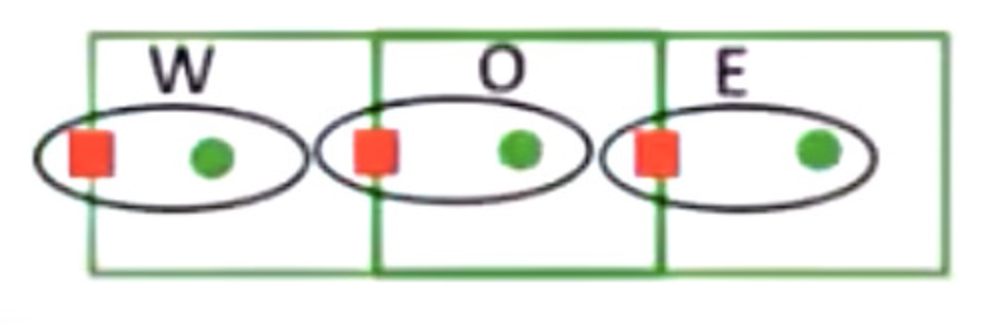
\includegraphics[height=0.085\textwidth]{1Dstaggered.png} \label{fig:Staggered}} \quad
  \subfigure[Collocated]{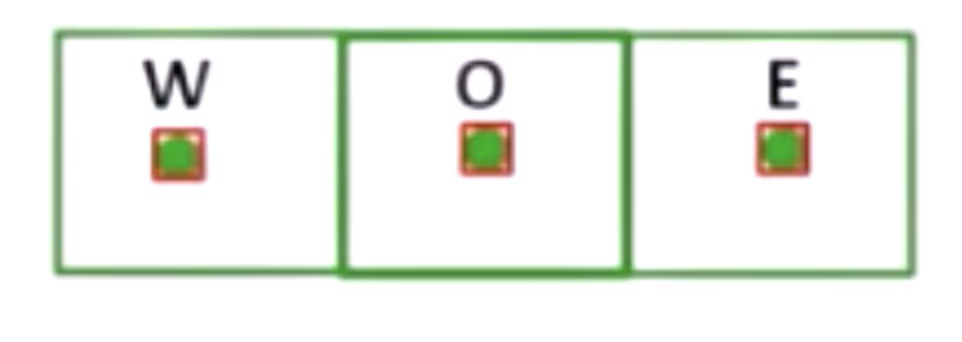
\includegraphics[height=0.095\textwidth]{1Dcollocated.png} \label{fig:Collocated}}
\caption{\small Staggered vs Collocated grids.}
\end{figure}

\subsection{Boundary conditions for pressure}\label{sec:boundary-conditions-for-pressure}

An interesting and important question arises as to what boundary conditions should be used for the pressure field. Such conditions are required at every point of the boundary for the Poisson problem to be well-posed 

Applying $(\nabla \cdot)$ to the momentum equation~\eqref{eqn:momentum}, first taking into account the commutativity of time derivative and Laplace operator $\nabla^2$ with $(\nabla \cdot)$, then eliminating these terms by applying continuity equation~\eqref{eqn:continuity}, finally leads to Poisson equation for pressure

\begin{equation}\label{eqn:pressure-poisson}
\nabla \cdot(\nabla p) \equiv \nabla^2 p=\rho \nabla \cdot[-\boldsymbol{v} \cdot \nabla \boldsymbol{v}].
\end{equation}



The conditions, however, do not naturally follow from the flow physics for the boundaries between fluid and solid walls. We have to find a way to derive the pressure boundary conditions from the equations themselves.

%\textbf{Is below needed?}

%For a moment consider a general Poisson equation $\Delta p = f$ on a bounded, sufficiently smooth domain $\Omega$ where $f$ is given and sufficiently regular. It is known that there exists 
%\begin{itemize}
%	\item A unique solution if a nonempty part of the boundary $\Gamma \subset\partial \Omega$ is given Dirichlet boundary conditions by specifying $\left.p\right|_{\Gamma}$ and the rest of the boundary is given Neumann boundary conditions by specifying $\left.\frac{\partial p}{\partial  \boldsymbol{n}}\right|_{\partial\Omega\setminus \Gamma}$
%	\item A solution which is unique up to a constant if we are given all Neumann boundary conditions by specifying $\left.\frac{\partial p}{\partial  \boldsymbol{n}}\right|_{\partial\Omega}$, and the compatibility condition $\int_{\partial\Omega} \frac{\partial p}{\partial  \boldsymbol{n}} = \int_\Omega f$ holds, which can be derived as follows:
%$$ \int_{\partial\Omega} \frac{\partial p}{\partial  \boldsymbol{n}} = \int_{\partial\Omega}\nabla p \cdot \boldsymbol{n} = \int_{\Omega}\nabla\cdot\nabla p = \int_\Omega \Delta p = \int_\Omega f;$$
%the solution becomes unique as long as we fix the value of $p$ at a single point in $\Omega$.
%\end{itemize}
%
%Now suppose instead that we start from a vector equation $\nabla p = \boldsymbol F$ in $\Omega$ and want to solve for $p$. Note that this equation only specifies $p$ up to a constant, so let's assume that there is some point $x_0 \in \partial\Omega$ where $p$ is specified. By taking the divergence of both sides, we get the Poisson equation $\Delta p = f$ for $f = \nabla\cdot\boldsymbol{F}$. What is a 'natural' boundary condition for this Poisson equation given the vector equation we started from? Since the boundary condition is a scalar, there is some freedom in how we do this. One way is to take the dot product with the normal vector $\boldsymbol{n}$ to get the Neumann condition $\left.\frac{\partial p}{\partial  \boldsymbol{n}}\right|_{\partial\Omega} = \left. \boldsymbol{F}\cdot \boldsymbol{n}\right|_{\partial\Omega};$ if this is the only condition, notice that the compatibility condition is automatically satisfied since
%
%$$ \int_{\partial\Omega} \frac{\partial p}{\partial  \boldsymbol{n}} = \int_{\partial\Omega}\boldsymbol{F} \cdot \boldsymbol{n} = \int_{\Omega}\nabla\cdot\boldsymbol{F}  = \int_\Omega f.$$
%
%
%Therefore we have a well-posed Poisson problem with Neumann boundary conditions. However, this is not necessarily the only condition we could derive. For example, in two dimensions say one could instead project the vector equation onto the tangent boundary vector $\boldsymbol \tau$ to give $\left.\frac{\partial p}{\partial  \boldsymbol{\tau}}\right|_{\partial\Omega} = \left. \boldsymbol{F}\cdot \boldsymbol{\tau}\right|_{\partial\Omega}$ which could be integrated along $\partial\Omega$ to give Dirichlet boundary conditions for $p$ (where we also need the value of $p$ at $x_0$ to uniquely determine the boundary values). This condition is obviously a bit more complex so not seen as often, but in the paper I cited they show that the derived Dirichlet and Neumann conditions for the PPE are in fact equivalent.



Recalling calculus: the gradient of any function $f$ is defined as the unique vector field whose dot product with any vector $v$ at each point $x$ is the directional derivative of $f$ along $v$, i.e. $\nabla f \cdot v=\frac{\partial f}{\partial v}$.

Consider $\boldsymbol{n}$ to be the normal vector to the solid wall boundary. We apply $(\cdot\boldsymbol{n})$ to the momentum equation~\eqref{eqn:momentum} and get

\begin{equation}\label{eqn:pressure-bc}
\left.\frac{\partial p}{\partial \boldsymbol{n}}\right|_{\partial \Omega}=\left.\rho\left[\nu \nabla\cdot\nabla \boldsymbol{v}-\frac{\partial \boldsymbol{v}}{\partial t}-\boldsymbol{v} \cdot \nabla \boldsymbol{v}\right] \cdot \boldsymbol{n}\right|_{\Omega}.
\end{equation}


To compute the pressure values at the boundaries we need to take into account the impermeability condition. The velocity component perpendicular to the wall is zero, meaning that the flow can not penetrate the wall, mathematically written as

\begin{equation}
	\label{eqn:impermeability}
		\boldsymbol{v}\cdot 	\boldsymbol{n}\bigg|_{\partial \Omega}=0.
\end{equation} 

By taking into account impermeability condition~\eqref{eqn:impermeability} equation~\eqref{eqn:pressure-bc} leads to boundary condition for the pressure at the wall computed as

\begin{equation}\label{eqn:pressure-wall}
	\begin{aligned}
		\left.\frac{\partial p}{\partial \boldsymbol{n}}\right|_{\partial \Omega}=\left.\rho\left[\nu \nabla\cdot\nabla \boldsymbol{v}-\frac{\partial \boldsymbol{v}}{\partial t}-\boldsymbol{v} \cdot \nabla \boldsymbol{v}\right] \cdot \boldsymbol{n}\right|_{\Omega}\implies
		\frac{\partial p}{\partial \boldsymbol{n}}\bigg|_{\partial \Omega}=\rho \left[\nu \nabla \cdot \nabla \boldsymbol{v}\right]\cdot \boldsymbol{n}\bigg| _{\partial \Omega}.
	\end{aligned}
\end{equation}

The diffusive term on the right-hand side is nonzero even after the application of no-slip conditions $\boldsymbol{v}\cdot\boldsymbol{t}\bigg|_{\partial \Omega}=0$ at the wall, where $\boldsymbol{t}$ is a tangential vector to the wall, i.e. diffusion at the wall is directed in the normal direction from the boundary.

%For inlets and outlets, an expression similar to above~\eqref{eqn:pressure-wall} can be obtained, which leads to $\frac{\partial p}{\partial n}$ at the boundary, and thus, the Poisson problem for pressure is defined up to a constant. There are, however, several techniques to overcome this issue numerically: fixing one pressure value at a single boundary node/cell, assuming some value then shifting the average value of the field to zero, etc.

Boundary conditions for pressure~\eqref{eqn:pressure-bc} and \eqref{eqn:pressure-wall} define a solution of the Poisson equation for pressure~\eqref{eqn:pressure-poisson} up to a constant, i.e. we need to fix value for $p$ at any point of our domain. Another method to obtain boundary conditions for pressure is to apply $(\boldsymbol{t}\cdot)$ to the momentum equation~\eqref{eqn:momentum} which will lead to Dirichlet boundary condition, where the value of pressure at a single point $x_0$ is also needed to uniquely determine the boundary values. Gresho \cite{Gresho:1987} describes the equivalence of the derived Dirichlet and Neumann conditions for the Pressure Poisson equation.

The results obtained for pressure boundary conditions require special treatment and recomputation for every change of velocity near the boundaries, which increases the complexity of solvers and generates more errors. Section~\ref{sec:vorticity-streamfunction} displays an approach that completely eliminates pressure from the problem statement, thus removing the requirement of its boundary conditions. 

%You have the right idea! One paper I find very helpful on the topic of the Pressure Poisson Equation (PPE) is [this one here][1]; it goes into the various formulations and boundary conditions and their relationships, as well as some numerical analysis related to boundary layers. I'll try to give useful context, and for ease of notation use $\Delta$ in place of $\nabla\cdot\nabla$ for the Laplacian.
%
%
%
%For a moment consider a general Poisson equation $\Delta p = f$ on a bounded, sufficiently smooth domain $\Omega$ where $f$ is given and sufficiently regular. It is known that there exists 
%
%(a) a *unique* solution if a nonempty part of the boundary $\Gamma \subset\partial \Omega$ is given Dirichlet boundary conditions by specifying $\left.p\right|_{\Gamma}$ and the rest of the boundary is given Neumann boundary conditions by specifying $\left.\frac{\partial p}{\partial  \boldsymbol{n}}\right|_{\partial\Omega\setminus \Gamma}$
%
%(b) a solution *unique up to a constant* if we are given all Neumann boundary conditions by specifying $\left.\frac{\partial p}{\partial  \boldsymbol{n}}\right|_{\partial\Omega}$, and the compatibility condition $\int_{\partial\Omega} \frac{\partial p}{\partial  \boldsymbol{n}} = \int_\Omega f$ holds, which can be derived as follows:
%$$ \int_{\partial\Omega} \frac{\partial p}{\partial  \boldsymbol{n}} = \int_{\partial\Omega}\nabla p \cdot \boldsymbol{n} = \int_{\Omega}\nabla\cdot\nabla p = \int_\Omega \Delta p = \int_\Omega f;$$
%the solution becomes unique as long as we fix the value of $p$ at a single point in $\Omega$.
%
%Now suppose instead that we start from a vector equation $\nabla p = \boldsymbol F$ in $\Omega$ and want to solve for $p$. Note that this equation only specifies $p$ up to a constant, so let's assume that there is some point $x_0 \in \partial\Omega$ where $p$ is specified. By taking the divergence of both sides, we get the Poisson equation $\Delta p = f$ for $f = \nabla\cdot\boldsymbol{F}$. What is a 'natural' boundary condition for this Poisson equation given the vector equation we started from? Since the boundary condition is a scalar, there is some freedom in how we do this. One way as you noticed is to take the dot product with the normal vector $\boldsymbol{n}$ to get the Neumann condition
%$\left.\frac{\partial p}{\partial  \boldsymbol{n}}\right|_{\partial\Omega} = \left. \boldsymbol{F}\cdot \boldsymbol{n}\right|_{\partial\Omega};$ if this is the only condition, notice that the compatibility condition is automatically satisfied since
%$$ \int_{\partial\Omega} \frac{\partial p}{\partial  \boldsymbol{n}} = \int_{\partial\Omega}\boldsymbol{F} \cdot \boldsymbol{n} = \int_{\Omega}\nabla\cdot\boldsymbol{F}  = \int_\Omega f.$$
%Therefore we have a well-posed Poisson problem with Neumann boundary conditions. However, this is not necessarily the only condition we could derive. For example, in two dimensions say one could instead project the vector equation onto the tangent boundary vector $\boldsymbol \tau$ to give $\left.\frac{\partial p}{\partial  \boldsymbol{\tau}}\right|_{\partial\Omega} = \left. \boldsymbol{F}\cdot \boldsymbol{\tau}\right|_{\partial\Omega}$ which could be integrated along $\partial\Omega$ to give Dirichlet boundary conditions for $p$ (where we also need the value of $p$ at $x_0$ to uniquely determine the boundary values). This condition is obviously a bit more complex so not seen as often, but in the paper I cited they show that the derived Dirichlet and Neumann conditions for the PPE are in fact equivalent.
%
%Now what about the PPE derived from Navier Stokes? It has the exact setup as before just with $\boldsymbol F = \rho\left[\nu \Delta \boldsymbol{v} - \frac{\partial \boldsymbol{v}}{\partial t} - \boldsymbol{v} \cdot \nabla \boldsymbol{v}\right]$ and the additional condition $\nabla\cdot \boldsymbol{v} = 0$. This divergence-free condition yields $\nabla\cdot \boldsymbol{F} = -\rho\nabla\cdot(\boldsymbol{v} \cdot \nabla \boldsymbol{v})$
%and so the PPE with 'natural' Neumann BCs is
%\begin{equation}
%\begin{aligned}
%\Delta p &= -\rho\nabla\cdot(\boldsymbol{v} \cdot \nabla \boldsymbol{v}) \\
%\\
%\left.\frac{\partial p}{\partial  \boldsymbol{n}}\right|_{\partial\Omega} &= \left. \rho\left[\nu \Delta \boldsymbol{v} - \frac{\partial \boldsymbol{v}}{\partial t} - \boldsymbol{v} \cdot \nabla \boldsymbol{v}\right]\cdot \boldsymbol{n}\right|_{\partial\Omega}
%\end{aligned}
%\end{equation}
%
%Notice we did not use any boundary conditions for $\boldsymbol v$ to come up with the PPE; it is well posed regardless of the possible choices for boundary conditions on the velocity since $\boldsymbol v$ is assumed to be a known fixed quantity. However, the impermeability condition $\boldsymbol v\cdot \boldsymbol n = 0$ leads to a slightly less complicated Neumann condition for $p$ since the middle term drops out.
%
%So you basically have all the right ideas, but hopefully with this additional context you can see that the PPE is in fact well-posed even with all Neumann boundary conditions
%
%
%  [1]: https://www.navier-stokes-equations.com/the-pressure-arte-fact;focus=CMTOI_de_dtag_hosting_hpcreator_widget_Download_10762411&path=download.action&frame=CMTOI_de_dtag_hosting_hpcreator_widget_Download_10762411?id=54674


\section{Marker-and-cell scheme}\label{sec:marker-and-cell-scheme}

The system \eqref{eqs:NSE} does not involve $\partial p / \partial t$, hence, the pressure cannot be advanced in time by means of its time derivative. In fact, the only place $p$ appears in the equations at all is in the pressure gradient term in the momentum equation~\eqref{eqn:momentum}. If this term were differenced in a purely explicit manner, the scheme would not involve $p^{n+1}$ in any way, so there would be no way to compute it. In order to advance the pressure in time, the temporal difference approximation to $\nabla p$ in \eqref{eqn:momentum} must be at least partially implicit so that $p^{n+1}$ appears in the difference scheme. This in turn implies that the temporal difference approximation to $\nabla \cdot \boldsymbol{v}$ in \eqref{eqn:continuity} must likewise be at least partially implicit since the difference
approximation to \eqref{eqn:momentum} alone does not provide enough equations to determine both $\boldsymbol{v}^{n+1}$ and $p^{n+1}$. But once $\nabla \cdot \boldsymbol{v}$ is partially implicit, it might as well be fully implicit, which entails no additional labour and has the significant advantage of satisfying \eqref{eqn:continuity} exactly at each time level
of the calculation. We, therefore, difference \eqref{eqn:momentum} in a fully implicit manner
\begin{align}
\label{eqn:continuity:MAC}
\left(\nabla \cdot \boldsymbol{v}\right)^{n+1} = 0.
\end{align}
The momentum equation can be differenced in a fully explicit manner except for the pressure gradient
\begin{align}
\label{eqn:momentum:MAC}
\frac{\boldsymbol{v}^{n+1}-\boldsymbol{v}^{n}}{\Delta t} + \left(\boldsymbol{v} \cdot \nabla \boldsymbol{v}\right)^{n} = - \nabla p^{*} + \nu \left(\nabla \cdot \nabla \boldsymbol{v}\right)^{n},
\end{align}
where $p^{*} = \gamma p^{n+1} + (1-\gamma) p^{n}$ with the weighting factor $0 < \gamma \le 1$ controlling the degree of implicitness of the scheme. The system (\eqref{eqn:continuity:MAC},\eqref{eqn:momentum:MAC}) is now closed that allows uniquely determine $\boldsymbol{v}^{n+1}$ and $p^{*}$ regardless of the value of $\gamma$. Varying $\gamma$ produces small changes of order of $\Delta t$ in the time history of the pressure field, but has no effect on the velocity field. The precise value of $\gamma$ is immaterial, therefore, we may well adopt the simplest choice $\gamma=1$ so that $p^{*}=p^{n+1}$, i.e. approximating the pressure gradient in a fully implicit manner. This choice constitutes the MAC scheme \cite{Harlow:1965}. Equations (\eqref{eqn:continuity:MAC},\eqref{eqn:momentum:MAC}) are ordinarily solved by iterative methods, of which the traditional choices were successive over-relaxation (SOR).

\todo{Include a section on Chorin's scheme \cite{Chorin:1968} before discussing a general view in \S \ref{sec:pressure-correction}.}

\section{Chorin's Projection Scheme}\label{sec:chorin}

%The system of Navier Stokes equations \eqref{eqs:NSE} using the Finite Difference Method in the bounded region $\mathfrak{D}$ as suggested by Chorin  is solved.

The proposed method by Chorin \cite{Chorin:1968} was solved on a staggered grid as illustrated in figure~\ref{fig:grid-staggered} using Finite Differences. The algorithn can be summarized as follows: the time $t$ is discretized, at every time step two separate equations are solved and combined based on the decomposition theorem of Ladyzhenskaya sometimes referred to as Helmholtz-Hodge Decomposition or simply as Hodge decomposition. The theorem states that the vector field $\mathbf{u}$ defined on a simply connected domain can be uniquely decomposed into a divergence-free (solenoidal) part ${\mathbf  {u}}_{{{\text{sol}}}}$ and an irrotational part ${\mathbf  {u}}_{{{\text{irrot}}}}$, leading to $\mathbf{u}={\mathbf  {u}}_{{{\text{sol}}}}+{\mathbf  {u}}_{{{\text{irrot}}}}$. In the case of Navier-Stokes equations, advection-diffusion terms from initial to intermediate time are considered as a divergence-free part and the pressure gradient at the time step from intermediate to last as an irrotational part. The method developed by Chorin is focused on solving two equations (Burgers' and Poisson), which are obtained after introducing intermediate velocity $\boldsymbol{\tilde v}$.
 
%\begin{itemize}
%	\item The component with zero divergence $-\boldsymbol{v} \cdot \nabla \boldsymbol{v} + \nu \nabla \cdot \nabla \boldsymbol{v}$,
%	\item The component with zero curl $-\nabla p$.
%\end{itemize}

Chorin's scheme was computed in single time step as follows:

\begin{enumerate}
%	\item Let initial guess $\boldsymbol{v}^0$ and the guesses at each time step $\boldsymbol{v}^n$ be divergence-free.
	\item Solve for intermediate velocity field $\boldsymbol{\tilde v}$ equation~\eqref{eqn:chorin-burgers}, generally not satisfying incompressible condition, since pressure gradient does not appear in
		\begin{equation}\label{eqn:chorin-burgers}
			\frac{\boldsymbol{\tilde v} - \boldsymbol{v}^n}{\Delta t}=-\boldsymbol{v}^n\cdot\nabla_d\boldsymbol{v}^n+\nu \Delta_d\boldsymbol{v}^n,
		\end{equation}
		where superscript denotes known values of $\boldsymbol{v}$ at $n$'th time step and subscript $d$ denotes discretized gradient and Laplacian operators.
		Chorin solved the above Burgers' equation~\eqref{eqn:chorin-burgers} using the alternating direction implicit method. 
	\item This step is based on the application of Helmholz-Decomposition to final velocity field $\boldsymbol{v}^{n+1}$,
		\begin{equation}\label{eqn:chorin-helmholz}
		\begin{aligned}
			\boldsymbol{v}^{n+1}&=\boldsymbol{\tilde v}-\nabla_d (\Delta tp^{n+1}).
		\end{aligned}
		\end{equation}
		By imposing the divergence operator to the above equation~\eqref{eqn:chorin-helmholz} and making use of the continuity~\eqref{eqn:continuity} at time step $n+1$ a discretized version of the pressure-Poisson equation~\eqref{eqn:pressure-poisson} is written as
		\begin{equation}\label{eqn:chorin-pressure}
			\Delta_d p^{n+1}=\frac{1}{\Delta t}\nabla_d\boldsymbol{\tilde v}.
		\end{equation}
		Pressure condition at the boundary as in section~\ref{sec:boundary-conditions-for-pressure} is
		\begin{equation}\label{eqn:chorin-pressure-bc}
			\boldsymbol{n} \cdot \nabla_d p^{n+1}=\boldsymbol{n} \cdot\left(-\frac{\boldsymbol{v}^{n+1}-\boldsymbol{v}^n}{\Delta t}-\left(\boldsymbol{v} \cdot \nabla_d \boldsymbol{v}\right)^n+\nu \Delta_d \boldsymbol{v}^n\right).
		\end{equation}
		Equation~\eqref{eqn:chorin-pressure} is solved with the corresponding boundary condition~\eqref{eqn:chorin-pressure-bc}. Chorin used the Successive Point Over-Relaxation method, however, any appropriate iterative/direct/multigrid approaches might be used.
	\item Use the solution for pressure from Step 2 and compute velocity at the next time step
		\begin{equation}\label{eqn:chorin-corrector}
			\boldsymbol{v}^{n+1}=\tilde{\boldsymbol{v}}-\Delta t \nabla_d p^{n+1}.
		\end{equation}
\end{enumerate}





%This decomposition exists and is uniquely determined whenever the initial value problem for the Navier-Stokes equations is well posed; it has also been extensively used in existence and uniqueness proofs for the solution of these equations.



\section{Pressure-correction methods: general view} \label{sec:pressure-correction}

\begin{figure}
\centering
  \subfigure[MAC]{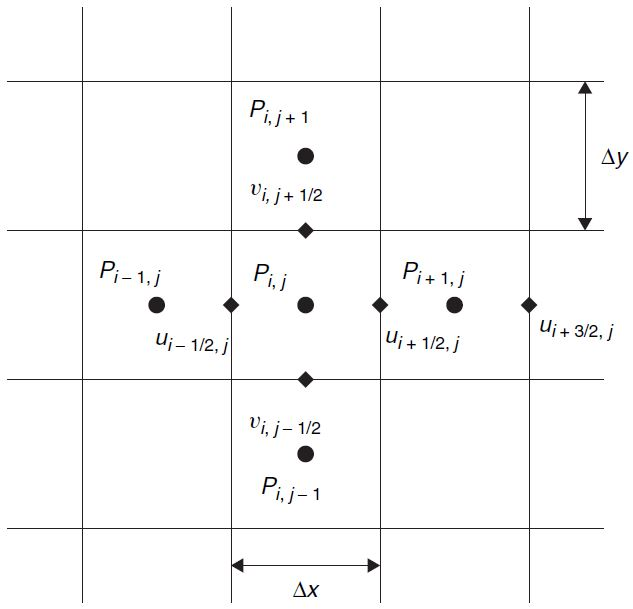
\includegraphics[height=0.295\textwidth]{grid-MAC.jpg} \label{fig:grid-MAC}} \quad
  \subfigure[general]{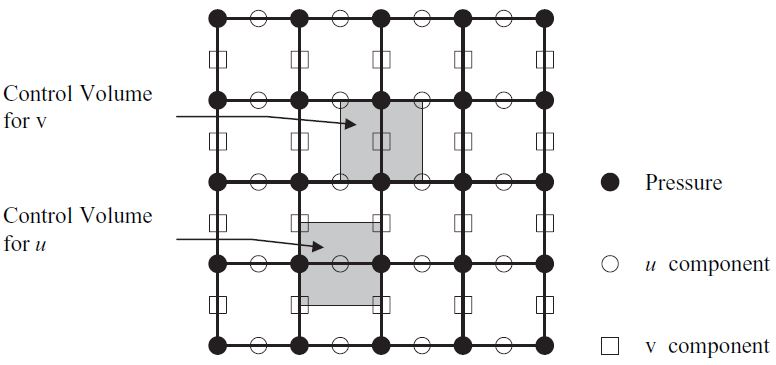
\includegraphics[height=0.295\textwidth]{grid-staggered.jpg} \label{fig:grid-staggered}}
\caption{\small Staggered grid.}
\end{figure}

As discussed by Dukowicz \& Dvinsky \cite{Dukowicz:1992}, both MAC \cite{Harlow:1965} and Chorin's \cite{Chorin:1968,Temam:1969a,Temam:1969b} methods can be put in a single form for time-discretization:
\begin{subequations}
\label{scheme:MAC-Chorin}
\begin{align}
\label{eqn:predictor}
\text{Predictor}&: & \frac{\widetilde{\boldsymbol{v}}-\boldsymbol{v}^{n}}{\Delta t} + \boldsymbol{v}^{n} \cdot \nabla \boldsymbol{v}^{*} &= \nu \nabla \cdot \nabla \boldsymbol{v}^{*}, \\
\label{eqn:corrector}
\text{Corrector}&: & 
\begin{split}
   \frac{\boldsymbol{v}^{n+1}-\widetilde{\boldsymbol{v}}}{\Delta t} &= -\nabla p^{*}, \\
   \nabla \cdot \boldsymbol{v}^{n+1} &= 0,
\end{split}
\end{align}
\end{subequations}
where $\Delta t$ is the time step and $\boldsymbol{v}^{*}$ stands for $\boldsymbol{v}^{n}$ in MAC and the intermediate velocity $\widetilde{\boldsymbol{v}}$ in Chorin's method; the pressure time level is unspecified in MAC and is taken to be the new time level by Chorin. The general strategy in \eqref{scheme:MAC-Chorin} is to decompose each time step into two substeps. On the first substep, the momentum equation is solved for the velocity components. The pressure gradient is
either removed from the equation or approximated by an estimate. The obtained velocity field cannot be considered a solution at the new time level since it does not satisfy the incompressibility condition. The second substep is, therefore, needed, at which the correct pressure distribution is found and the correction of velocity is made.

If one adopts the \textit{projection} point of view, as inspired by the existence theory of the NSEs, then the scheme \eqref{scheme:MAC-Chorin} can be interpreted as a projection of the intermediate velocity field $\widetilde{\boldsymbol{v}}$ onto a subspace of vector fields with zero divergence. Namely, the term projection reflects
the fact that we find a preliminary solution, which is not divergence-free, and then project it onto the space of divergence-free vector functions. This projection point of view, pioneered by Chorin \cite{Chorin:1968} is based on the observation that equation \eqref{eqn:momentum} can be put in the form $\frac{\partial \boldsymbol{v}}{\partial t} + \nabla p = - \boldsymbol{v} \cdot \nabla \boldsymbol{v} + \nu \nabla \cdot \nabla \boldsymbol{v}$, the left-hand side of which is a Hodge decomposition, so that by acting with the operator $\boldsymbol{P}$, which projects a vector field onto the space of divergence-free vector fields with appropriate boundary conditions, we get $\frac{\partial \boldsymbol{v}}{\partial t} = \boldsymbol{P}\left[- \boldsymbol{v} \cdot \nabla \boldsymbol{v} + \nu \nabla \cdot \nabla \boldsymbol{v}\right]$, which is the continuous version of \eqref{eqn:predictor}. On the other hand, the scheme \eqref{scheme:MAC-Chorin} can be interpreted from the \textit{operator-splitting} or \textit{fractional time-step} (aka \textit{time-splitting}) point of view on, which originates as a purely numerical method which is general and not specific to a particular set of equations \cite{Yanenko:1971}, since by adding the two sets of equations to eliminate the intermediate velocity $\widetilde{\boldsymbol{v}}$. Regardless of which point of view to take in order to interpret \eqref{scheme:MAC-Chorin}, the conceptual and practical advantage of decoupling the ``pressure correction'' from the momentum equation calculations.

\todo{\begin{itemize}
        \item \st{Add a section on spatial discretization using} \S 4.5 in \cite{Biringen:2011} as well as research papers \cite{Dukowicz:1992,Kim:1985,Perot:1993,Brown:2001}, etc. Use the notations for discrete advection, Laplacian, divergence, and gradient operators as per equation (3) in Perot \cite{Perot:1993}.
\\The articles listed describe time discretization techniques, and spatial operators are kept arbitrary. 
        \item Also discuss other numerical schemes in detail such as the \st{semi-implicit method for pressure linked equations (SIMPLE}) \cite{Patankar:1972,Patankar:1980}, \st{the pressure implicit with splitting of operators (PISO)} \cite{Issa:1985,Issa:1986}, Colonius' (discrete streamfunction), etc.
        \item Add a section on velocity-vorticity methods (\S 10.5.1 \cite{Zikanov:2010}, \S 4.6 \cite{Biringen:2011}).
        \item Since the scheme \eqref{scheme:MAC-Chorin} is first-order accurate in time, discuss its improvements in terms of accuracy \cite{Kim:1985,Dukowicz:1992,Perot:1993,Brown:2001}.
        \item When a reference is made to specific schemes such as the Crank-Nicholson, Adams-Bashforth, and so on, for self-contained discussion their description should be included in an appendix.
\end{itemize}}
	
	
	\section{Spatial Discretization}
	
	The initial system of equations~\eqref{eqs:NSE} can be rewritten using discrete spatial operators as
	\begin{equation}\label{eqs:discrete-NSE}
		\begin{gathered}
		\frac{\partial\boldsymbol{v}}{\partial t}+\mathbf{H}\left(\boldsymbol{v}\right)=-G p^{n+1}+\nu L\left(\boldsymbol{v}\right)
		%+\left(b \cdot c^{\prime} s\right)
		,\\
		D \mathbf{\boldsymbol{v}}^{n+1}=0,%+\left(b \cdot c^{\prime} s\right)
		\end{gathered}
	\end{equation}
	where $\mathbf{H}, G, L, D$ are discrete convective, gradient, Laplacian and divergence operators respectively.
	
	Bringen and Chow \cite{Biringen:2011} performed discretization on  uniform staggered MAC grid illustrated on figure~\ref{fig:grid-MAC} 
%	using $\Delta x = \Delta y = h$ 
	and used the discrete operators at time step $n$:
	\begin{equation}
		\begin{aligned}
			\mathbf{H}(\phi^n_{i+1/2,j},\psi^n_{i,j+1/2})&= \left(   
			\frac{\left(\phi_{i,j}^n\right)^2-\left(\phi_{i+1,j}^n\right)^2}{\Delta x}+
			\frac{(\phi\psi)_{i+1/2,j-1/2}^n-(\phi\psi)_{i+1/2, j+1/2}^n}{\Delta y}		
			\right. ,\\
			& \left. 
			\frac{(\phi \psi)_{i-1/2,j+1/2}^n-(\phi\psi)_{i+1/2,j+1/2}^n}{\Delta x}+
			\frac{\left(\psi_{i,j}^n\right)^2-\left(\psi_{i,j+1}^n\right)^2}{\Delta y} 
			\right),\\
			\left(G_x(\phi^n_{i+1/2,j}),G_y(\phi^n_{i,j+1/2})\right)&= \left(
				\frac{\phi^n_{i+1,j}-\phi^n_{i,j}}{\Delta x},		
				\frac{\phi^n_{i,j+1}-\phi^n_{i,j}}{\Delta y}
			\right),\\
			L(\phi^n_{i+1/2,j},\psi^n_{i,j+1/2})&=\left( 
				\frac{\phi_{i+3/2,j}^n-2 \phi_{i+1/2,j}^n+\phi_{i-1/2,j}^n}{\Delta x^2}+
				\frac{\phi_{i+1/2,j+1}^n-2 \phi_{i+1/2,j}^n+\phi_{i+1/2,j-1}^n}{\Delta y^2}
			\right. , \\
			&\left. 
				\frac{\psi_{i+1,j+1/2}^n-2\psi_{i,j+1/2}^n+\psi_{i-1,j+1/2}^n}{\Delta x^2} 	+
				\frac{\psi_{i,j+3/2}^n-2\psi_{i,j+1/2}^n+\psi_{i,j-1/2}^n}{\Delta y^2} 
			\right),\\
			D(\phi^n_{i,j},\psi^n_{i,j})&=\left(
				\frac{\phi^n_{i+1/2,j}-\phi^n_{i-1/2,j}}{\Delta x}+		
				\frac{\psi^n_{i,j+1/2}-\psi^n_{i,j-1/2}}{\Delta y}
			\right),
		\end{aligned}
	\end{equation}
	where $\phi,\psi$ are physical quantities. In the case of velocities they are evaluated at the cell surface leading to $1/2$ indices appearing, whereas for pressure the quantities are computed at the cell centre (marker). Convective operator $\mathbf{H}$ was evaluated in a conservative form 
	
	\begin{equation}
		\mathbf{H}(\boldsymbol{v})=\mathbf{H}(u,v)=\left(\frac{\partial u^2}{\partial x}+\frac{\partial u v}{\partial y},\frac{\partial u v}{\partial x}+\frac{\partial v^2}{\partial y}\right).
	\end{equation}
	
%	Need to keep in mind that above operators $\mathbf{H}, G, L, D$ 
	

	
	
	
	\subsection{Magnetization formulation, not needed?}
	
	
	An alternative formulation of the incompressible Navier–Stokes equations~\eqref{eqs:NSE} based on a new variable called "magnetization", “impulse,” or “gauge” can be made~\cite{Brown:2001}. Two new variables, $\boldsymbol{m}$ and $\chi$, are introduced that are related to the fluid velocity by
$$
\boldsymbol{m}=\boldsymbol{v}+\nabla \chi.
$$
The vector field $\boldsymbol{m}$ and the potential $\chi$ can be chosen to satisfy evolution equations in such a way that the fluid velocity and pressure derived from them satisfy the Navier-Stokes equations. Given $\boldsymbol{m}$, one possibility is to let $\boldsymbol{m}$ satisfy in $\Omega$ the evolution equation
$$
\begin{aligned}
\boldsymbol{m}_t+(\boldsymbol{v} \cdot \nabla) \boldsymbol{v} &=\nu \nabla^2 \boldsymbol{m} \\
\left.\boldsymbol{v}\right|_{\partial \Omega} &=\boldsymbol{v}_b,
\end{aligned}
$$
where $\boldsymbol{v}=\mathbf{P}(\boldsymbol{m})$ is the operator which projects a vector field onto the space of divergence-free vector fields with appropriate boundary conditions.
	

\section{Modern schemes for solving Navier-Stokes equations}

This section is focused on several popular methods described in two-dimensional cases.

\subsection{SIMPLE - Semi-Implicit Method for Pressure Linked Equations}

As discussed in section~\ref{sec:oscillations-on-collocated} there is a possibility that a solution on collocated grids will generate spurious oscillations due to interpolation, the use of staggered grids can address this issue. One of the methods on staggered grids was developed by Patankar and Spalding~\cite{Patankar:1972}. They named it SIMPLE, algorithm was based on a predictor-corrector procedure with successive pressure correction

\begin{equation}\label{eqn:simple-pressure}
	p = 	\bar p + p',
\end{equation}
where $p$ is the actual pressure, $\bar p$ is the estimated pressure, and $p'$ is the pressure correction. Similarly to the pressure correction~\eqref{eqn:simple-pressure} , the velocity vector is decomposed into two terms
\begin{equation}\label{eqn:simple-velocity}
	\boldsymbol{v}=\boldsymbol{\bar v}+\boldsymbol{v}'=(\bar u + u', \bar v + v').
\end{equation}

Corrections of pressure are related to the velocity corrections by approximate momentum equation,

\begin{equation}\label{eqn:simple-apx-mom}
%\begin{aligned}
\frac{\partial \boldsymbol{v}'}{\partial t}=-Gp\implies \boldsymbol{v}'=-G ( p\Delta t).
%\rho \frac{\partial u^{\prime}}{\partial t} &=-\frac{\partial p^{\prime}}{\partial x}\\
%\rho \frac{\partial v^{\prime}}{\partial t} &=-\frac{\partial p^{\prime}}{\partial y}
%\end{aligned}
%\quad\implies\quad
%\begin{aligned}
%&u^{\prime}=-\frac{\Delta t}{\rho} \frac{\partial p^{\prime}}{\partial x} \\
%&v^{\prime}=-\frac{\Delta t}{\rho} \frac{\partial p^{\prime}}{\partial y}.
%\end{aligned}
\end{equation}

Combining velocity correctiion \eqref{eqn:simple-velocity} with right hand side of expression \eqref{eqn:simple-apx-mom} and substituting the result into the continuity equation~\eqref{eqn:continuity}, we obtain the so-called pressure-correction Poisson equation


\begin{equation}\label{eqn:simple-poisson}
%p_{, i i}^{\prime}=-\frac{\rho}{\Delta t}\left(\frac{\partial \mathrm{v}_i}{\partial x_i}-\frac{\partial \overline{\mathrm{v}}_i}{\partial x_i}\right)=\frac{\rho}{\Delta t} \frac{\partial \overline{\mathrm{v}}_i}{\partial x_i}, \quad(i=1,2),\quad 
DGp'\equiv\nabla\cdot\nabla p'=-\frac{1}{\Delta t}\left( D \boldsymbol{v}-D\boldsymbol{\bar v} \right)=\frac{1}{\Delta t}D\boldsymbol{\bar v},
\end{equation}
where we set $\nabla\cdot\boldsymbol{v}=0$ to enforce the mass conservation at the current time step. An iterative procedure used to obtain the solution is described below.

\begin{enumerate}
	\item \label{simple:1} Guess the pressure $\bar{p}$ distribution at each cell centre.
	\item \label{simple:2} Solve the momentum equation in control volumes formulation at the staggered grid points $(i+1 / 2$, $i-1 / 2, j+1 / 2, j-1 / 2)$ to find $\boldsymbol{\bar v}$.
	\item \label{simple:3} Solve the pressure correction equation \eqref{eqn:simple-poisson} to find $p'$ at integer points $(i, j),(i, j-1)$, $(i, j+1),(i-1, j),(i+1, j)$. The corner grid points are avoided, therefore, the scheme is called "semi-implicit".
	\item \label{simple:4} Correct the pressure and velocity using the equations~\eqref{eqn:simple-pressure},\eqref{eqn:simple-velocity} and \eqref{eqn:simple-apx-mom}:
		\begin{equation}
			\begin{aligned}
				p&=\bar p + p',\\
				\boldsymbol{v}&=\boldsymbol{\bar v}-\Delta t\left[Gp'-\mathbf{H}(\boldsymbol{v}')+\nu L(\boldsymbol{v}')\right].
			\end{aligned}
		\end{equation}
	\item \label{simple:5} Replace the previous intermediate values of pressure and velocity $\left(\bar{p}, \boldsymbol{\bar{v}}\right)$ with the corrected values $\left(p, \boldsymbol{v}\right)$ and return to Step \ref{simple:2} .
	\item \label{simple:6} Repeat Steps \ref{simple:2} to \ref{simple:5} until desired convergence is achieved.
\end{enumerate}

There are several modifications of the current method that lead to better convergence.  These algorithms were named SIMPLER (SIMPLE revised) and SIMPLEC (SIMPLE consistent), with SIMPLEC being the most effective scheme. 
%(a) Guess the pressure $\bar{p}$ at each grid point.
%(b) Solve the momentum equation to find $\overline{\mathbf{v}}_i$ at the staggered grid $(i+1 / 2$, $i-1 / 2, j+1 / 2, j-1 / 2)$, discretized in control volumes and control surfaces (Section 1.4) as shown in Figure 5.3.1.
%(c) Solve the pressure correction equation (5.3.5) to find $p^{\prime}$ at $(i, j),(i, j-1)$, $(i, j+1),(i-1, j),(i+1, j)$. Since the corner grid points are avoided, the scheme is "semi-implicit," not fully implicit, as shown in Figure 5.3.1.
%(d) Correct the pressure and velocity using (2.2.9b), (5.3.2), and (5.3.4).
%$$
%\begin{aligned}
%p &=\bar{p}+p^{\prime} \\
%u &=\bar{u}-\frac{\Delta t}{2 \rho \Delta x}\left(p_{i+1, j}^{\prime}-p_{i-1, j}^{\prime}\right)-\frac{\Delta t}{\rho}\left(A_{i+\frac{1}{2}, j}^{(1)}-A_{i-\frac{1}{2}, j}^{(1)}\right) \\
%\mathbf{v} &=\overline{\mathrm{v}}-\frac{\Delta t}{2 \rho \Delta y}\left(p_{i, j+1}^{\prime}-p_{i, j-1}^{\prime}\right)-\frac{\Delta t}{\rho}\left(A_{i, j+\frac{1}{2}}^{(2)}-A_{i, j-\frac{1}{2}}^{(2)}\right)
%\end{aligned}
%$$
%where
%$$
%\begin{array}{ll}
%A^{(1)}=\left(\rho \mathrm{v}_k^{\prime} \mathrm{v}_1^{\prime}\right)_{, k}-\mu\left(\mathrm{v}_{1, k k}^{\prime}+\frac{1}{3} \mathrm{v}_{k, k 1}^{\prime}\right) & (k=1,2) \\
%A^{(2)}=\left(\rho \mathrm{v}_k^{\prime} \mathrm{v}_2^{\prime}\right)_{, k}-\mu\left(\mathrm{v}_{2, k k}^{\prime}+\frac{1}{3} \mathrm{v}_{k, k 2}^{\prime}\right) & (k=1,2)
%\end{array}
%$$
%with $\mu$ being the dynamic viscosity.
%(e) Replace the previous intermediate values of pressure and velocity $\left(\bar{p}, \bar{v}_i\right)$ with the new corrector values $\left(p, \mathrm{v}_i\right)$ and return to $(\mathrm{b})$.
%(f) Repeat Steps (b) through (e) until convergence.

\subsection{PISO - Pressure Implicit with Splitting of Operators}


Issa \cite{Issa:1985,Issa:1986} proposed an additional correction step to the SIMPLE algorithm. The sequential procedure is described below.
\begin{enumerate}
	\item \label{piso:1} Set ${p}^n$, $\boldsymbol{v}^n$ from previous timestep.
	\item \label{piso:2} Solve the momentum equation in control volumes formulation at the staggered grid points $(i+1 / 2$, $i-1 / 2, j+1 / 2, j-1 / 2)$ to find $\boldsymbol{v'}$.
			\begin{equation}
				\frac{1}{\Delta t} \left( \boldsymbol{v'} - \boldsymbol{v}^n\right) = -\mathbf{H}(\boldsymbol{v}) + \nu L(\boldsymbol{v})-G\bar p.
			\end{equation}
	\item \label{piso:3} Solve first pressure correction equation \eqref{eqn:simple-poisson} to find $p'$ at integer points $(i, j),(i, j-1)$, $(i, j+1),(i-1, j),(i+1, j)$, the equation below has conservation of mass enforced $\nabla\cdot\boldsymbol{v}'=0$. 
			\begin{equation}
				DGp''\equiv\nabla \cdot \nabla p' = -\frac{1}{\Delta t}\left( \nabla \cdot \boldsymbol{v}' - \nabla\cdot \boldsymbol{v}^n\right)=\frac{1}{\Delta t}\left(\nabla\cdot \boldsymbol{v}^n\right)=\frac{1}{\Delta t}D\boldsymbol{v}^n .
			\end{equation}
	\item \label{piso:4} Apply first correction and obtain $\boldsymbol{v}''$ from
			\begin{equation}
				\frac{1}{\Delta t}\left( \boldsymbol{v}'' - \boldsymbol{v}^n\right) = D(-\mathbf{H}(\boldsymbol{v}') + \nu L(\boldsymbol{v}'))-G(p').
			\end{equation}
	\item \label{piso:5} Solve the second pressure correction
			\begin{equation}
				DGp''\equiv\nabla\cdot\nabla p'' = \frac{1}{\Delta t}\ D\boldsymbol{v}+D\left(-\mathbf{H}(\boldsymbol{v}'') + \nu L(\boldsymbol{v}'')\right).
			\end{equation}
	\item \label{piso:6} Apply second correction and obtain $\boldsymbol{v}'''=\boldsymbol{v}^{n+1}$ from
			\begin{equation}
				\frac{1}{\Delta t} \left(\boldsymbol{v}''' - \boldsymbol{v}^n \right)=-\mathbf{H}(\boldsymbol{v}'') + \nu L(\boldsymbol{v}'')
			\end{equation}
\end{enumerate}

\section{Discrete streamfunction method}\label{sec:discrete-streamfunction}
%%%%%%%%%%%%%%%%%%%%%%%%%%%%%%%%%%%%%%%%%%%%%%%%%%%%%%%%%%%%%%%%%%%%%%
%There are a few things to add/clarify:
%1. Non-dimensionalization.
%2. BC discussion (analytic).
%3. Symmetric BC on top to be included in all operators. 
%4. Scaling of G and D operators. 
%5. Indexation change.
%%%%%%%%%%%%%%%%%%%%%%%%%%%%%%%%%%%%%%%%%%%%%%%%%%%%%%%%%%%%%%%%%%%%%%
\todo{
\begin{itemize}
%    \item \st{Non-dimensionalization.} \st{Shall we keep u component under value of 1? can multiply the freestream and inlet by 0.5 if needed.} Normalized to max value of 1.
%	\item \st{Scaling of G and D operators.} \textit{$\left(C^T\right)\left(\hat{M}\right)\left(\hat{G}\right)p=\left(C^T\right)\left(\hat{M}\right)\left(\hat{M}^{-1}{G}\right)p=C^TGp=(-DC)^Tp=0$.}
%    \item \st{Symmetric BC on top to be included in all operators.}
%    \item \st{Indexing change for equations and figures.}
    \item \st{Motivation.} Added some, where possible!
    \item \st{BC discussion (analytic).} \cite{Engquist:1977,Kourta:1987,Liu:1993,Sani:1994,Persillon:1998,Tsynkov:1998}.
    \item \st{Outlet diffusion discretization is problematic. Requested PhD thesis of Jin and Persillon through UofA library. Wrote an email to their supervisor Prof. Braza and sent a message to Persillon.} Waiting for the response form UofA library since 11th Dec. 
%    \item \st{Substitute all refs/eqrefs with smart \textbackslash cref and use one bracket for \textbackslash cite.} 
%    \item Is it ok to use "Sys. (43)" for SLAE?
%    \item \st{Time step $n$ is in superscript, however, domain dim's are $n\times m$, dimension index is in subscript.} Changed dimensions to $M\times N$
%    \item Outlet idea 1. (headache division by zero) might be using uniform grid in the direction of the flow and refine grid only vertically. Will use three-point scheme into the domain, but then matrix L becomes asymmetric. 
%	\item Outlet idea 2. Use extrapolation $\frac{\partial ^2 \boldsymbol{v}}{\partial x^2}=0$ or BC by Kourta $\frac{\partial ^2u}{\partial x^2}=0,\frac{\partial v}{\partial x	}=0$.
    \item  \st{Found this condition $\frac{\partial \boldsymbol{v}}{\partial t}+u \frac{\partial \boldsymbol{v}}{\partial x}+v \frac{\partial \boldsymbol{v}}{\partial y}-\nu \frac{\partial^2 \boldsymbol{v}}{\partial y^2}=0$ by G. Fournier and F. Golanski (2008, but not many citations). They claim Prandtl BL solution for advective bc $\frac{\partial \boldsymbol{v}}{\partial t} + u\frac{\partial \boldsymbol{v}}{\partial x}=0$ is wrong, while their solution matches Prandtl BL. Looks like we can express the remaining diffusive summand in terms of pressure gradient at the boundary.} Wrote an email to author, waiting for the response. 
    \item \st{Change computational domain to inner part only? Boundary values are to be determined by BC, not the momentum eq'n, contrary to Hall}\cite{Hall:1980}. Changed unknowns to inner part only. Values at the boundary are determined using BC. 
    \item \st{Check algebra of diffusion and advection for $v$ component.} 
    \item It feels like BC scheme which is consistent with inner discretization won't work, we will use Jin-Braza scheme. 
  \end{itemize}
}

\subsection{Problem statement}\label{subsec:problem-statement-dimentional}
Let the velocity vector $\boldsymbol{v}(t,x,y)=(u(t,x,y),v(t,x,y))$ and pressure $p(t,x,y)$ be the solutions to ~\cref{eqs:NSE} on a semi-infinite domain together with boundary conditions:
\begin{subequations}
\label[pluralequation]{eqs:NSE-dsm-bl-dimensional}
\begin{align}
\label{eqn:momentum-dimensional}
\text{Momentum: }	&\frac{\partial \boldsymbol{v}}{\partial t} + \boldsymbol{v} \cdot \nabla \boldsymbol{v} = -\frac{1}{\rho}\nabla p + {\frac{\mu}{\rho}} \nabla \cdot \nabla \boldsymbol{v},\\
&\rho\text{ - density}, \mu\text{ - dynamic viscosity.}\notag\\
\label{eqn:continuity-dsm-bl}
\text{Continuity: }	& \nabla \cdot \boldsymbol{v} = 0, \\ 
					&0\leq x < \infty, 0\leq y <\infty, t\geq0.\notag\\
\label{eqn:NSE-dsm-bl-bc-freestream}
\text{Inlet and Freestream BC: } 	& \boldsymbol{v}(t,0,y)=\boldsymbol{v}(t,x,\infty)=\left(U_0 + A\cos\left( kx -\omega t + \phi_0 \right),0\right),\\
									& \{|A|<U_0,k,\omega, \phi_0\}\subset \mathbb{R}.\notag\\
\label[bc]{eqn:NSE-dsm-bl-bc-noslip}
\text{No-slip BC: } & \boldsymbol{v}(t,x,0)=(0,0). \\
%\label{eqn:NSE-dsm-bl-bc-outlet}
%\text{Outlet BC: } 	& \frac{\partial u}{\partial t}+u\frac{\partial u}{\partial x}=0\lor\left(\frac{\partial u}{\partial t}+u\frac{\partial u}{\partial x}=\nu \frac{\partial ^2 u}{\partial y^2}\right), \\ 
%					& v=\boldsymbol{h}(t,y)-\text{linear extrapolation},\notag\\
%					& (x=\infty),\notag\\
\text{Initial condition: } &\boldsymbol{v}(0,x,y)=(0,0).
\end{align}
\end{subequations}

\subsection{Artificial boundary conditions}\label{sec:artificial-bc}
Though there are methods that may solve problems on unbounded domains, the majority of the algorithms can only be applied to finite ones. 
%In case of a truncated domain, the introduction of appropriate artificial boundary conditions (ABCs) is crucial for achieving numerical solutions. 
The review papers on such BCs by Sani~\cite{Sani:1994} and Tsynkov~\cite{Tsynkov:1998} list and compare different artificial boundary conditions (ABC) applied to the various flow scenarios. Below we will discuss the options that are most applicable to \cref{eqs:NSE-dsm-bl-dimensional}. 

In solutions of fluid flow, the reflection of waves at the outlet is common. Such behaviour is due to the elliptic nature of the incompressible Navier-Stokes. Engquist introduced one of the earliest and successful methods to address this problem. The corresponding paper~\cite{Engquist:1977} demonstrates the application of this method to both wave and shallow water equations. Although the method is not fully applicable to our problem, the authors systematically addressed and resolved the reflective behaviour of the outlet.
\begin{figure}[H] % here, bottom, top
  \centering{
  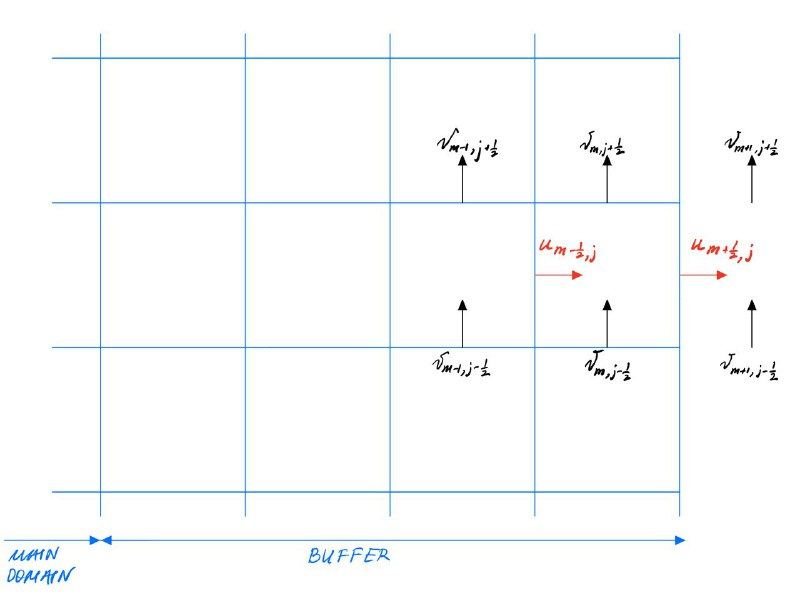
\includegraphics[width=0.5\paperwidth]{BC-Buffer}
  }
  \caption{Buffer BC by Liu.}\label{fig:BC-buffer}
\end{figure}
Another way of overcoming the reflective behaviour of the fluid flow was developed by Liu~\cite{Liu:1993}. They studied the spatial instability of planar Poiseuille flow. The governing equations in this paper were solved for perturbed velocity components with tilde $\tilde{u}=u-u_0,\tilde{v}=v-v_0$, where $u_0,v_0$ are mean values of velocity components $u,v$. The general idea is the introduction of an additional buffer domain (\cref{fig:BC-buffer}) at the exit that involves the use of:
\begin{enumerate}
	\item Semi-implicit perturbed mass conservation
	\begin{equation*}
		\tilde{u}_{m+\frac{1}{2},j}^{n+1}=\tilde{u}_{m-\frac{1}{2},j}^n-\frac{\tilde{v}^n_{m-1,j+\frac{1}{2}}-\tilde{v}^n_{m-1,j-\frac{1}{2}}}{\Delta y_{j}}{\Delta x_m}.
	\end{equation*}
	\item Zero change in acceleration of the tangential perturbed velocity component computed semi-implicitly as
	\begin{equation*}
		\frac{\partial ^2 \tilde{v}}{\partial x^2}=0\implies \tilde{v}^{n+1}_{m+1,j-\frac{1}{2}}=2\tilde{v}^n_{m,j-\frac{1}{2}}-\tilde{v}^n_{m-1,j-\frac{1}{2}},
	\end{equation*}
	where $\tilde{v}^{n+1}_{m+1,j-\frac{1}{2}}$ is the ghost component outside the domain.
\end{enumerate}
This buffer was not consistent with the physics and required to be as short as possible. 

Braza and collaborators~\cite{Jin:1993,Kourta:1987,Persillon:1998} considered the shear flow (mixing layer) problem. Authors developed a set of BCs that allows the eddies to be freely developed downstream as they leave the domain. Furthermore, the most appropriate boundary conditions at the top and bottom were those derived by considering boundaries as streamlines with
\begin{equation}\label[bc]{eqn:symmetric-bc}
	v=0\text{ and } \frac{\partial u}{\partial y}=0,
\end{equation}
while the non-reflective outlet had the following boundary conditions: 
\begin{subequations}
\label[pluralequation]{eqs:braza}
\begin{align}
\label[bc]{eqn:kourta-bc}
	\text{Type I: }&\frac{\partial ^2u}{\partial x^2}=0,\frac{\partial v}{\partial x	}=0,\\
\label[bc]{eqn:jin-bc}
	\text{Type II: }&\frac{\partial \boldsymbol{v}}{\partial t}+u\frac{\partial \boldsymbol{v}}{\partial x}-\nu \frac{\partial^2 \boldsymbol{v}}{\partial y^2}=0,
\end{align}
\end{subequations}
where $\nu$ is kinematic viscosity. 
Results shown in \cref{fig:kourta-results,fig:jin-results} correspond to results obtained through \cref{eqn:kourta-bc,eqn:jin-bc}.
	The first \cref{eqn:kourta-bc} made vortices hit against a "wall", while they went out of the domain. 
	However, the second \cref{eqn:jin-bc} was derived similarly to Engquist~\cite{Engquist:1977} from wave equation and displayed more non-reflective behaviour. 
	In addition, the numerical algorithm used in the corresponding paper~\cite{Jin:1993} required boundary conditions for auxiliary potential function $\phi$ at the outlet. 
	The corresponding ABC for $\phi$ was derived from the numerical algorithm by taking into account \cref{eqn:jin-bc}. 
	(It might be possible to obtain an ABC for pressure depending on the algorithm used.)
\begin{figure}
\centering
  \subfigure[Kourta-Braza results.]{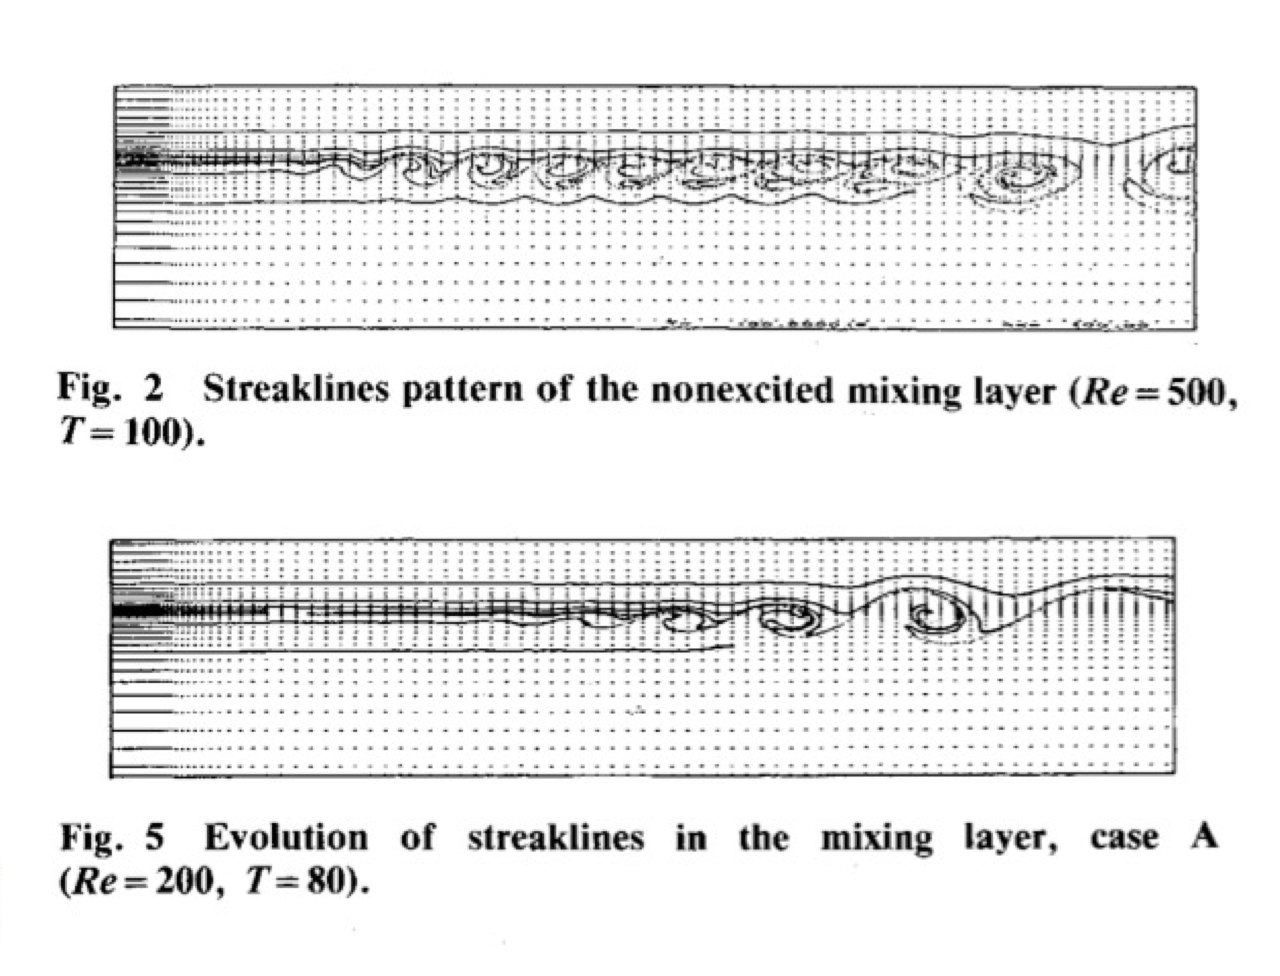
\includegraphics[height=0.265\textwidth]{Braza-Kourta.jpg} \label{fig:kourta-results}} \quad
  \subfigure[Jin-Braza results.]{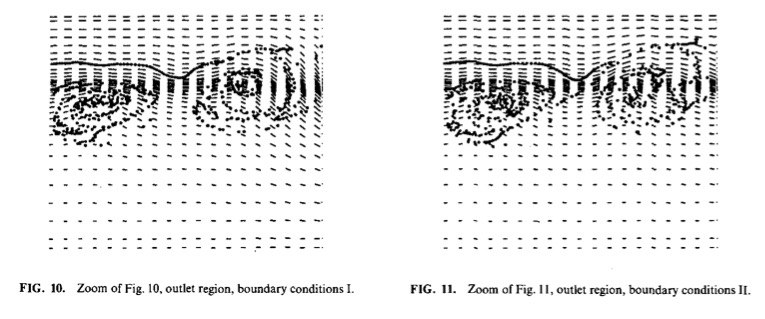
\includegraphics[height=0.245\textwidth]{Braza-Jin.jpg} \label{fig:jin-results}}
\caption{\small Resultant streaklines of Braza and collaborators.}
\end{figure}

Taking into account successful results obtained in \cite{Kourta:1987, Jin:1993, Persillon:1998} and similarities between the boundary layer and mixing layer flows we will use\footnote{G. Fournier and F. Golanski (2008) claim that Prandtl BL solution for advective BCs s.a. $\frac{\partial \boldsymbol{v}}{\partial t} + u\frac{\partial \boldsymbol{v}}{\partial x}=0$ results in wrong solution for pressure gradient, while their condition $\frac{\partial \boldsymbol{v}}{\partial t}+u \frac{\partial \boldsymbol{v}}{\partial x}+v \frac{\partial \boldsymbol{v}}{\partial y}-\nu \frac{\partial^2 \boldsymbol{v}}{\partial y^2}=0$ matches Prandtl BL.} \cref{eqn:jin-bc,eqn:symmetric-bc} as boundary conditions for top and right boundaries respectively and also truncate the domain to width and height $L$.

\subsubsection{Derivation of Type II ABC (as in paper)}\label{subsubsec:non-reflecting-abc}
Velocity vector $\boldsymbol{v}$ is considered as the transported wave quantity incident on the boundary. 
Due to the elliptic nature of the flow, the boundary is said to satisfy the anisotropic wave equation
\begin{equation}\label{eqn:wave-eqn-at-bdry}
	\frac{\partial ^2 \boldsymbol{v}}{\partial t^2}-c_x^2\frac{\partial ^2 \boldsymbol{v}}{\partial x^2}-c_y^2\frac{\partial ^2 \boldsymbol{v}}{\partial y^2}=0,
\end{equation}
where $c_x,c_y$ are the characteristic velocities of $x,y$ wave propagation. 

We can rewrite \cref{eqn:wave-eqn-at-bdry} in terms of pseudo-differential operators
\begin{equation*}
	L\boldsymbol{v}\equiv -D_t^2\boldsymbol{v}+c_x^2D_x^2\boldsymbol{v}+c_y^2D_y^2\boldsymbol{v=0},
\end{equation*}
where $D^2_x,D^2_y$ and $D^2_t$ are second derivatives w.r.t. $x,y$ and $t$ variables respectively. 

Operator $L$ can be factored into
\begin{equation*}
	L\boldsymbol{v}=L^+L^-\boldsymbol{v}=0,
\end{equation*}
where
\begin{align*}
	L^+&\equiv c_x D_x + D_t\sqrt{1-\left( \frac{c_y D_y}{D_t}\right)^2},\\
	L^-&\equiv c_x D_x - D_t\sqrt{1-\left( \frac{c_y D_y}{D_t}\right)^2}\\
\end{align*}
correspond to waves travelling inside and outside the domain in directions parallel to the $x$ axis. 

To nullify the reflected waves, a total absorption~\cite{Engquist:1977} at the boundary
\begin{equation}\label{eqn:absorb-incoming}
	L^+\boldsymbol{v}=0
\end{equation}
is considered. It is possible to use the Taylor series to approximate the square root term, however, the results were found to be strongly ill posed, whereas, Pade second approximation
\begin{equation}\label{eqn:pade-second}
	\sqrt{1-\left( \frac{c_y D_y}{D_t}\right)^2}\approx1-\frac{1}{2}\left( \frac{c_y D_y}{D_t}\right)^2
\end{equation}
turned out to be well posed~\cite{Engquist:1977,Kreiss:1970} . It is possible to rewrite \cref{eqn:absorb-incoming} in terms of \cref{eqn:pade-second} as
\begin{equation*}
	\left( c_xD_x + D_t - \frac{c^2_y}{2D_t}D_y^2 \right)\boldsymbol{v}=0,
\end{equation*}
which can be matched to the momentum Navier-Stokes equation as
\begin{equation}\label[bc]{eqn:absorbing-bc-dimensional}
	\frac{\partial \boldsymbol{v}}{\partial t} + u\frac{\partial \boldsymbol{v}}{\partial x}-\frac{1}{\operatorname{Re}}\frac{\partial ^2 \boldsymbol{v}}{\partial y^2}=0.
\end{equation}



%\subsubsection{Top BC}\label{subsubsec:top-bc}

\subsection{Nondimensionalization}\label{subsec:Nondimensionalization}
In numerical computations, it is advantageous to maintain variables of comparable magnitude. This ensures that operations such as the multiplication of a large dimensional pressure variable with a small velocity are not performed. 

We will truncate the domain and normalize all equations by width $L$ and stream velocity $U_0$. After introducing the following dimensionless variables (marked with prime ${ }^{\prime}$ ):
\begin{equation*}
	x\to Lx^{\prime},  \quad 
	\boldsymbol{v}\to U_0\boldsymbol{v}^{\prime}, \quad 
	\nabla\to \frac{1}{L}\nabla^{\prime}, \quad 
%	\Delta \to \frac{1}{L^2} \Delta^{\prime},  \quad 
	p\to p^{\prime} \rho U_0^2, \quad 
	t\to \frac{L}{U_0}t^{\prime},
\end{equation*}
we obtain
\begin{equation*}
	\frac{U_0}{\frac{L}{U_0}} \frac{\partial \boldsymbol{v}^{\prime}}{\partial t^{\prime}}+U_0\boldsymbol{v}\cdot\left(\frac{1}{L} \nabla^{\prime}\right) U_0\boldsymbol{v}=-\frac{1}{\rho}\left(\frac{1}{L} \nabla^{\prime}\right){p^{\prime}\rho U^2_0}+\frac{\mu}{\rho} \left(\frac{1}{L} \nabla^{\prime}\right) \cdot\left(\frac{1}{L} \nabla^{\prime}\right) U_0\boldsymbol{v}^{\prime}.
\end{equation*}
After multiplying both sides of the equation by $\frac{L}{U_0^2}$ and introducing well-known Reynolds number 
\begin{equation*}
\operatorname{Re}=\frac{\rho L U_0}{\mu},
\end{equation*}
we obtain the non-dimensional momentum equation
\begin{equation*}
	\frac{\partial \boldsymbol{v}}{\partial t} + \boldsymbol{v} \cdot \nabla \boldsymbol{v} = -\nabla p + \frac{1}{\operatorname{Re}} \nabla \cdot \nabla \boldsymbol{v},
\end{equation*}
where prime superscript $\prime$ is suppressed for the dimensionless variables. The continuity equation is nondimensionalized in a similar manner:
\begin{equation*}
	\left(\frac{1}{L} \nabla^{\prime}\right) \cdot U_0\boldsymbol{v}^{\prime}=0\iff\nabla^{\prime} \cdot\boldsymbol{v}^{\prime}=0\implies\nabla \cdot\boldsymbol{v}=0,
\end{equation*}
where we drop prime superscripts in the last identity as well.


\subsection{Problem statement on truncated domain}
The initial \cref{eqs:NSE-dsm-bl-dimensional} from \cref{subsec:problem-statement-dimentional} on semi-infinite domain now become a system of partial differential equations on a unit square domain 
\begin{subequations}
\label[pluralequation]{eqs:NSE-dsm-bl}
\begin{align}
\label{eqn:momentum}
\text{Momentum: }	&\frac{\partial \boldsymbol{v}}{\partial t} + \boldsymbol{v} \cdot \nabla \boldsymbol{v} = -\nabla p + \nu \nabla \cdot \nabla \boldsymbol{v}, \\ 
					&\nu = \frac{1}{\operatorname{Re}},0\leq x \leq 1, 0\leq y \leq 1, t\geq0.\notag\\
\label{eqn:continuity-dsm-bl}
\text{Continuity: }	& \nabla \cdot \boldsymbol{v} = 0, \\ 
					&0\leq x \leq 1, 0\leq y \leq 1, t\geq0. \notag\\
\label[bc]{eqn:NSE-dsm-bl-bc-freestream}
\text{Inlet and Freestream BC: } 	& \boldsymbol{v}(t,0,y)=\boldsymbol{v}(t,x,1)=\left(1 + A\cos\left( kx -\omega t + \phi_0 \right),0\right),\\
									& \{A\leq 1,k,\omega, \phi_0\}\subset \mathbb{R}.\notag\\
\label[bc]{eqn:NSE-dsm-bl-bc-noslip}
\text{No-slip BC: } & \boldsymbol{v}(t,x,0)=(0,0). \\
\label[bc]{eqn:NSE-dsm-bl-bc-outlet}
\text{Outlet BC: } 	&\frac{\partial \boldsymbol{v}}{\partial t}+u\frac{\partial \boldsymbol{v}}{\partial x}-\nu \frac{\partial^2 \boldsymbol{v}}{\partial y^2}=0, \\ 
%					& v=\boldsymbol{h}(t,y)-\text{linear extrapolation},\notag\\
					& (x=1).\notag\\
\text{Initial condition: } &\boldsymbol{v}(0,x,y)=(0,0).
\end{align}
\end{subequations}

\subsection{Domain discretization}\label{subsec:dsm-domain}
Following the successful nondimensionalization of the governing equations, we now turn our attention to the process of domain discretization. This crucial step involves dividing the computational domain into discrete elements, allowing us to compute variables and their derivatives on a finite set of points called grid. Consider discretizing the area into $M$ intervals horizontally and $N$ intervals vertically forming a mesh of rectangular cells. To enhance memory access, it is recommended to organize the data using arrays instead of matrices. In this section, however, for the sake of simplicity, we use two indices $i,j$ (column and row as in Harlow~\cite{Harlow:1965}) to represent coordinates on the grid.

\begin{figure}[H] % here, bottom, top
  \centering{
  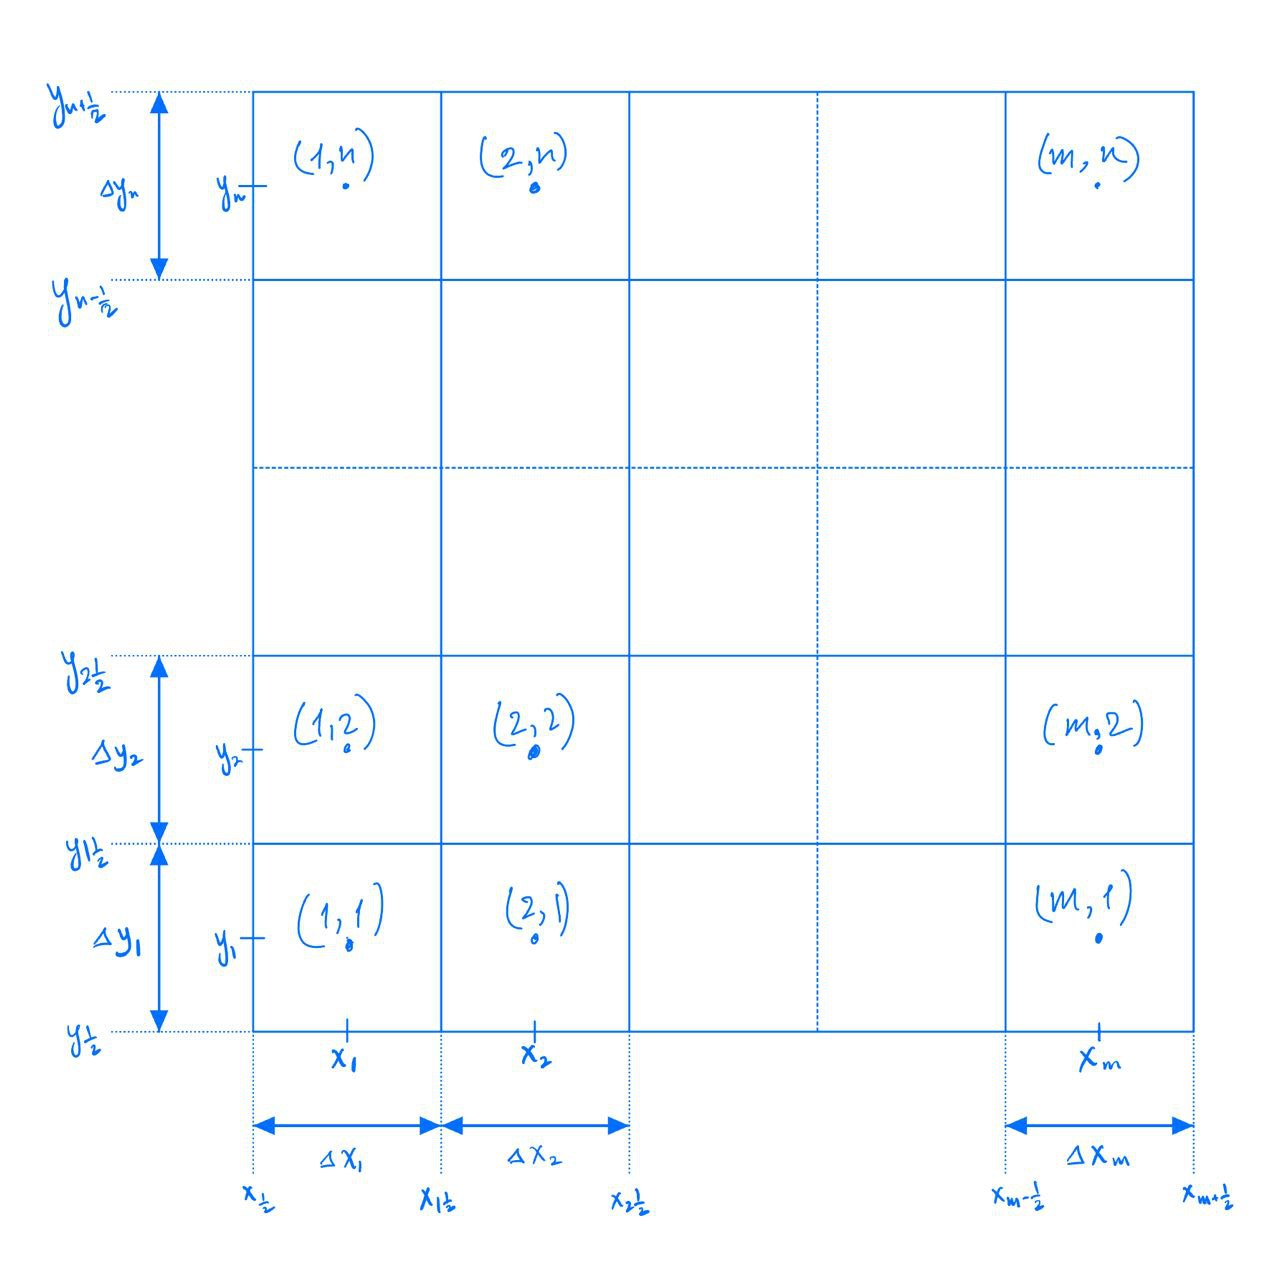
\includegraphics[width=0.45\paperwidth]{grid-bl}
  }
  \caption{Domain discretization}\label{bl-domain-discretization}
\end{figure}

To eliminate the necessity of solving an additional equation for pressure we will be using a staggered grid arrangement. 
Moreover, the pressure gradients can be evaluated directly using central differences on such grids. 
This calculation does not require any interpolation on staggered grids, furthermore, it is computationally cheaper and simple. 
Details are discussed in \cref{subsec:divergence,subsec:gradient,sec:nullspace-method}. 
The $u$ velocity components are stored at the centres of vertically oriented faces, while the values of $v$ are stored at the centres of horizontal ones. 

The number of unknown components inside the domain (excluding boundaries) is $M(N-1)$ for $v$ and $(M-1)N$ for $u$. In \cref{eqn:NSE-dsm-bl-bc-outlet}, the values of $u$ for the outlet are not explicitly defined. To address this, we will express the values on the boundary using \cref{eqn:NSE-dsm-bl-bc-outlet} in terms of data from inner part of the domain. These arrays for $u$ and $v$ are then concatenated into a single vector $\boldsymbol{v}$ of size $M(N-1)+(M-1)N$.

Increasing the accuracy closer to the wall and the outlet does look advantageous, hence, we will refine the grid using the standard ratio rule $\Delta x_{i+1}=k_x\Delta x_i,\Delta y_{j+1}=k_y\Delta y_j$ with constants $k_x,k_y$ close to the value of $1$. Grid indexation starts at $(x_{\frac{1}{2}},y_{\frac{1}{2}})=(0,0)$ and ends at $(x_{M+\frac{1}{2}},y_{N+\frac{1}{2}})=(1,1)$. The intervals $\Delta x, \Delta y$ have the same indexation as the corresponding cells they belong to. 

%%%%%%%%%%%%%%%%%%%%%%%%%%%%%%%%%%%%%%%%%%%%%%%%%%%%%%%%
\subsection{Discrete operators}

This subsection focuses on the specific operators used in the discretization of \cref{eqs:NSE-dsm-bl}, providing the mathematical tools necessary to transform these continuous equations into a form that can be solved numerically.

Initial system of \cref{eqs:NSE-dsm-bl} can be approximated using discrete spatial operators as

\begin{equation}\label[system]{eqn:nse-matrix}
            \begin{bmatrix}
                  \mathbf{I} && 0 \\ 
                  0 && 0
            \end{bmatrix}
            \frac{\partial }{\partial t} 
            \begin{pmatrix}
                  \boldsymbol{v} \\ 
                  p
            \end{pmatrix}
            =
            \begin{bmatrix}
                  \hat{L} && - \hat{G} \\ 
                  -\hat{D} && 0
            \end{bmatrix}
            \begin{bmatrix}
                  \boldsymbol{v} \\
                  p
            \end{bmatrix}
            +
            \begin{pmatrix}
                  -\mathbf{\hat{H}}(\boldsymbol{v})\\
                  0
            \end{pmatrix} + \text{bc}_{\boldsymbol{v},p},
        \end{equation}
where boundary conditions are in terms of pressure and velocity. In the following subsections, each of the discrete operators is described individually. 

%%%%%%%%%%%%%%%%%%%%%%%%%%%%%%%%%%%%%%%%%%%%%%%%%%%%%%%%%%%
%\subsubsection{Transient terms}\label{subsec:transient}
Attack \cref{eqn:nse-matrix} with the following schemes as in Colonius~\cite{Colonius:2008} (superscript denotes the time step):
\begin{enumerate}
	\item[\textbf{Viscous}] - Implicit trapezoidal - Crank Nicholson scheme (second-order method in time).  
%	\begin{equation}\label{eqn:crank-nicholson}
%		\frac{\boldsymbol{v}^{n+1}-\boldsymbol{v}^n}{\Delta t}=\frac{1}{2}\left[F^{n+1}+F^n\right],
%	\end{equation}
	\begin{equation}\label{eqn:viscous-crank-nicholson}
  		\hat{L}\boldsymbol{v}=\frac{1}{2}\left(\hat{L}\boldsymbol{v}^{n+1}+\hat{L}\boldsymbol{v}^n\right)
	\end{equation}

	\item[\textbf{Nonlinear}] - Explicit Adams-Bashforth (second-order method in time).
%	\begin{equation}\label{eqn:adams-bashforth}
%		\frac{\boldsymbol{v}^{n+1}-\boldsymbol{v}^{n}}{\Delta t} = \frac{3}{2}F^{n} - \frac{1}{2}F^{n-1}.
%	\end{equation}
	\begin{equation}\label{eqn:nonlinear-adams-bashforth}
		\mathbf{\hat{H}}(\boldsymbol{v}) = \frac{3}{2}\mathbf{\hat{H}}(\boldsymbol{v}^{n}) - \frac{1}{2}\mathbf{\hat{H}}(\boldsymbol{v})^{n-1}.
	\end{equation}

	\item[\textbf{Pressure}] - Implicit Euler, though the pressure variable will be later eliminated in the algorithm (first-order method in time). 
%	\begin{equation}\label{eqn:implicit-euler} 
%		\frac{\boldsymbol{v}^{n+1}-\boldsymbol{v}^{n}}{\Delta t} = F^{n+1}.
%	\end{equation}
	\begin{equation}\label{eqn:pressure-implicit-euler} 
		\hat{G}p = \hat{G}p^{n+1}.
	\end{equation}
\end{enumerate}

The above schemes result in the following time-discretized system:
\begin{equation}\label[system]{eqn:NSE-dsm-bl-system-schemes}
	\begin{bmatrix}
		\frac{1}{\Delta t}\mathbf{I}-\frac{1}{2}\hat{L} & \hat{G} \\
		\hat{D} & 0
	\end{bmatrix}
	\begin{pmatrix}
		\boldsymbol{v}^{n+1} \\ 
		p^{n+1}
	\end{pmatrix}
	=
	\begin{pmatrix}
		\left[\frac{1}{\Delta t}\mathbf{I}-\frac{1}{2}\hat{L}\right] \boldsymbol{v}^n - \left[\frac{3}{2}\hat{\mathbf{H}}(\boldsymbol{v}^n) - \frac{1}{2}\hat{\mathbf{H}}(\boldsymbol{v}^{n-1})\right]\\
		0
	\end{pmatrix}
	+
	\begin{pmatrix}
		\hat{bc}_1\\
		\hat{bc}_2
	\end{pmatrix}
\end{equation}
and \cref{eqn:jin-bc} 
\begin{equation}\label[bc]{eqn:jin-bc-transient-consistent}
\begin{gathered}
\frac{\boldsymbol{v}^{n+1}-\boldsymbol{v}^n}{\Delta t}+\left[\frac{3}{2}{u^n}\left(\frac{\partial \boldsymbol{v}}{\partial x}\right)^{n}-\frac{1}{2}{u^{n-1}}\left(\frac{\partial \boldsymbol{v}}{\partial x}\right)^{n-1}\right] \\
=\nu\left[\left(\frac{\partial^2 \boldsymbol{v}}{\partial y^2}\right)^{n+1}+\left(\frac{\partial^2 \boldsymbol{v}}{\partial y^2}\right)^{n}\right],
\end{gathered}
\end{equation}
however, the results produced with such \cref{eqn:jin-bc-transient-consistent} schemes are yet to be known and should be compared with \cref{eqn:jin-bc-transient} from the corresponding paper of Jin\cite{Jin:1993}, which was said to be 
\begin{equation}\label[bc]{eqn:jin-bc-transient}
\begin{gathered}
\frac{\boldsymbol{v}^{n+1}-\boldsymbol{v}^n}{\Delta t}+\frac{u^n}{2}\left[\left(\frac{\partial \boldsymbol{v}}{\partial x}\right)^{n+1}+\left(\frac{\partial \boldsymbol{v}}{\partial x}\right)^n\right] \\
=\nu\left(\frac{\partial^2 \boldsymbol{v}}{\partial y^2}\right)^n.
\end{gathered}
\end{equation}
We will first use discretized \cref{eqn:jin-bc-transient} from Jin~\cite{Jin:1993} as it was shown to be stable and produced solid results. Later on we can proceed with discretized \cref{eqn:jin-bc-transient-consistent} which is consistent with our schemes after developing the necessary techniques.

After applying the discrete operators listed in the following \cref{subsec:advection,subsec:laplacian,subsec:divergence,subsec:gradient}, we rewrite \cref{eqn:NSE-dsm-bl-system-schemes}  as
\begin{equation}\label[system]{eqn:NSE-dsm-bl-system-nonint}
	\begin{bmatrix}
		\hat{A} & \hat{G} \\
		\hat{D} & 0
	\end{bmatrix}
	\begin{pmatrix}
		\boldsymbol{v}^{n+1} \\ 
		p^{n+1}
	\end{pmatrix}
	=
	\begin{pmatrix}
		\hat{r}^n \\
		0
	\end{pmatrix}
	+
	\begin{pmatrix}
		\hat{bc}_1\\
		\hat{bc}_2
	\end{pmatrix},
\end{equation}
where $\hat{r}^n$ includes viscous, non-linear and gradient terms from time steps $n,n-1$ and $\hat{bc}_i$ are explicit boundary values in terms of velocity and pressure.


%%%%%%%%%%%%%%%%%%%%%%%%%%%%%%%%%%%%%%%%%%%%%%%%%%%%%%%%%%%
\subsubsection{Laplacian}\label{subsec:laplacian}

As per \cref{eqn:NSE-dsm-bl-system-schemes} it is required to approximate implicit viscous terms spatially. In order to obtain the discrete operator acting on a velocity vector we will rewrite Laplacian as a block matrix:
\begin{equation*}
	\hat L=
	\begin{bmatrix}
  \hat{L}^u_{xx}+\hat{L}^u_{yy} & 0 \\
  0 & \hat{L}^v_{xx}+\hat{L}^v_{yy}
\end{bmatrix}.
\end{equation*}

Each pair of the matrices $\hat{L}^u_{xx},\hat{L}^v_{xx}$ and $\hat{L}^u_{yy},\hat{L}^v_{yy}$ will be equal on a uniform, but different on non-uniform grids. These matrices are computed similarly. Below we will discuss how the Laplacian matrix is constructed at different parts of the grid.

\textbf{Inner part.}
The uniform grid refinement $\Delta x_{i+1}=k_x\Delta x_i,\Delta y_{j+1}=k_y\Delta y_j$ makes the order of the scheme consistent throughout the whole domain. Without loss of generality, let us show how to compute $\hat{L}^u_{xx}$. The other three matrices can be constructed in a similar manner. The power series of of $u_{i-\frac{1}{2}\pm 1,j}$ at nodes $x_{i - \frac{1}{2}\pm 1}$ with respect to $u_{i - \frac{1}{2},j}$ at node $x_{i-\frac{1}{2}}$ are
\begin{equation}\label{eqn:Taylor right} 
	u_{i-\frac{1}{2}+1,j}=u_{i-\frac{1}{2},j}+\left.\frac{\partial u}{\partial x}\right|_{i-\frac{1}{2},j}\left(x_{i-\frac{1}{2}+1}-x_{i-\frac{1}{2}}\right)+\frac{1}{2}\left.\frac{\partial^2 u}{\partial x^2}\right|_{i-\frac{1}{2},j}\left(x_{i-\frac{1}{2}+1}-x_{i-\frac{1}{2}}\right)^2+O\left(\Delta x^3\right),
\end{equation}
\begin{equation}\label{eqn:Taylor left} 
	u_{i-\frac{1}{2}-1,j}=u_{i-\frac{1}{2},j}+\left.\frac{\partial u}{\partial x}\right|_{i-\frac{1}{2},j}\left(x_{i-\frac{1}{2}-1}-x_{i-\frac{1}{2}}\right)+\frac{1}{2}\left.\frac{\partial^2 u}{\partial x^2}\right|_{i-\frac{1}{2},j}\left(x_{i-\frac{1}{2}-1}-x_{i-\frac{1}{2}}\right)^2+O\left(\Delta x^3\right).
\end{equation}
We can combine \cref{eqn:Taylor left,eqn:Taylor right} by cancelling the first derivative, which will result in
\begin{align}\label{eqn:laplacian-discretization-non-uniform-dx}
\left.\frac{\partial^2 u}{\partial x^2}\right|_{i-\frac{1}{2},j} & \approx \frac{u_{i-\frac{1}{2}+1,j}\left(x_{i-\frac{1}{2}}-x_{i-\frac{1}{2}-1}\right)-u_{i-\frac{1}{2},j}\left(x_{i-\frac{1}{2}+1}-x_{i-\frac{1}{2}-1}\right)+u_{i-\frac{1}{2}-1,j}\left(x_{i-\frac{1}{2}+1}-x_{i-\frac{1}{2}}\right)}{\left(\frac{x_{i-\frac{1}{2}+1}-x_{i-\frac{1}{2}-1}}{2}\right)\left(x_{i-\frac{1}{2}}-x_{i-\frac{1}{2}-1}\right)\left(x_{i-\frac{1}{2}+1}-x_{i-\frac{1}{2}}\right)}+O(\Delta x)\notag\\
& \approx \frac{1}{h_c h_e}u_{i-\frac{1}{2}+1} - \frac{2}{h_w h_e}u_{i-\frac{1}{2}} + \frac{1}{h_c h_w}u_{i-\frac{1}{2}-1} + O(\Delta x),
\end{align}
where $h_w=x_{i-\frac{1}{2}}-x_{i-\frac{1}{2}-1},h_c = \frac{x_{i-\frac{1}{2}+1}-x_{i-\frac{1}{2}-1}}{2}, h_e = x_{i-\frac{1}{2}+1}-x_{i-\frac{1}{2}}$ as in \cref{fig:luxx-inner}. The coefficients in front of the velocity components are then placed into the $\hat{L}^u_{xx}$ matrix. The order of this approximation becomes $2^{\text {nd }}$ for uniform grids. 

\begin{figure}[H] % here, bottom, top
  \centering{
  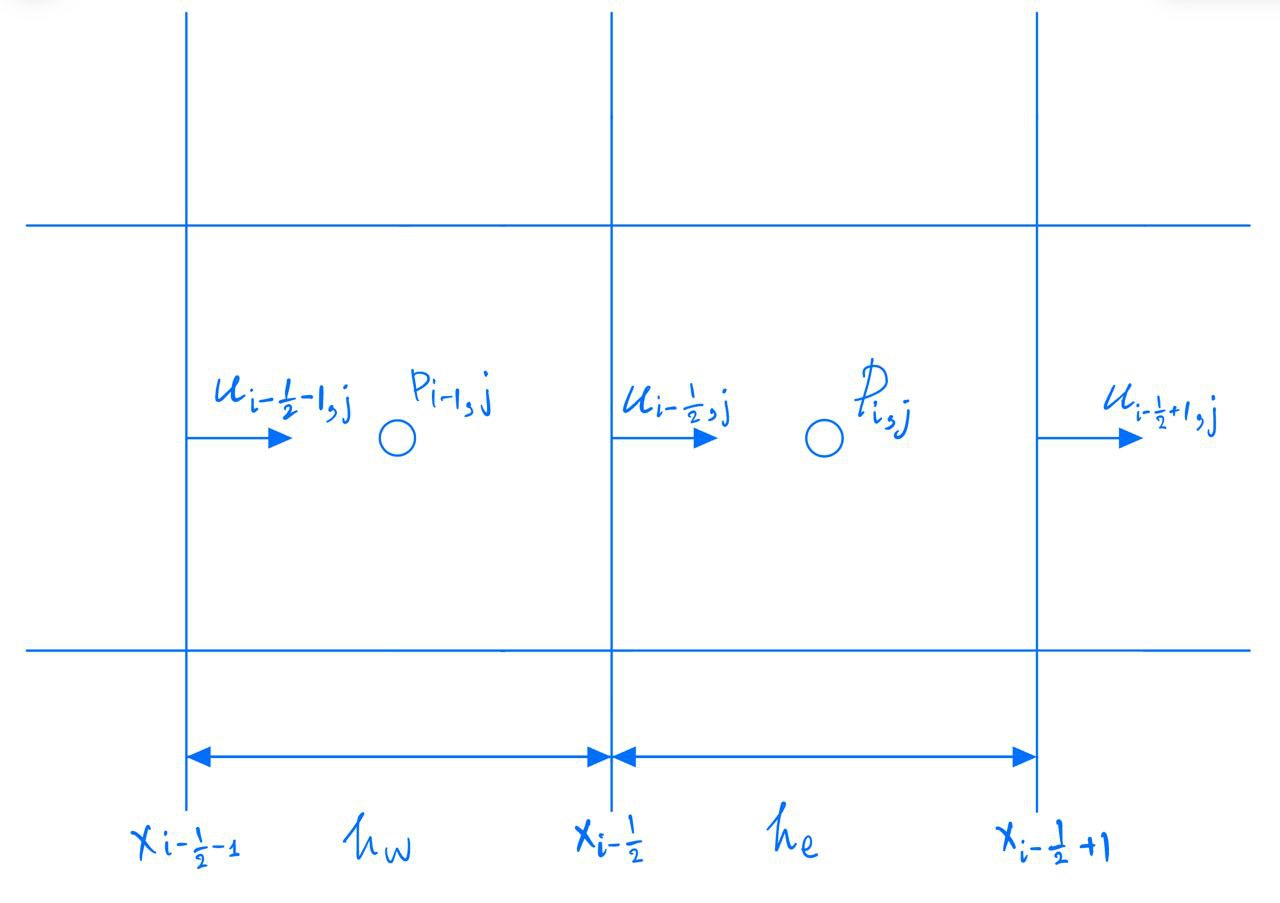
\includegraphics[width=0.45\paperwidth]{Luxx}
  }
  \caption{$\hat{L}^u_{xx}$ inner part.}\label{fig:luxx-inner}
\end{figure}
%The discretization for such grids is reduced to 
%\begin{equation}\label{eqn: second derivative uniform}
%\left(\frac{\partial^2 u}{\partial x^2}\right)_i \approx \frac{u_{i+1}-2 u_i+u_{i-1}}{(\Delta x)^2} + O(\Delta x^2).
%\end{equation}


\textbf{Right boundary.} 
%The aim is to make a second order scheme for the first derivative to keep consistency with the discretization of the inner part. Take the right most nodes, the aim is to eliminate the second derivative in equations below, cross multiply by coefficients to make up a common factor at second derivative, then subtract the equations. 
%	\begin{equation}
%	\begin{aligned}
%	& u_m=u_{m+1}+\left.\left(x_m-x_{m+1}\right) \frac{\partial u}{\partial x}\right|_{m+1}+\left.\frac{\left(x_m-x_{m+1}\right)^2}{2 !} \frac{\partial^2}{\partial x^2}\right|_{m+1}+\ldots \bigg/\frac{\left(x_{m-1}-x_{m+1}\right)^2}{2}. \\
%	& u_{m-1}=u_{m+1}+\left.\left(x_{m-1}-x_{m+1}\right) \frac{\partial u}{\partial x}\right|_{m+1}+\left.\frac{\left(x_{m-1}-x_{m+1}\right.}{2 !} \frac{\partial^2}{\partial x^2}\right|_{m+1}+\ldots \bigg/ \frac{\left(x_m-x_{m+1}\right)^2}{2}.
%	\end{aligned}
%	\end{equation}
%
%After subtracting and simplifying the expression for the first partial derivative reduces to
%\begin{equation}
%\frac{\partial u}{\partial x}\bigg|_{m+1}=\frac{-u_{m-1}{\left(x_m-x_{m+1}\right)^2}+u_m{\left(x_{m-1}-x_{m+1}\right)^2}-u_{m+1}{\left(x_{m-1}-x_m\right)\left(\left[x_{m-1}-x_{m+1}\right]+\left[x_m-x_{m+1}\right]\right)}}{{\left(x_m-x_{m+1}\right)\left(x_{m-1}-x_{m+1}\right)\left(x_{m-1}-x_m\right)}}.
%\end{equation}
%
%By applying simple Neumann boundary condition $\frac{\partial u}{\partial x}\big|_{m+1}=0$ we can express the right most value of the velocity with respect to the other two as
%\begin{equation}
%u_{m+1}=\frac{-u_{m-1}\left(x_m-x_{m+1}\right)^2+u_m\left(x_{m-1}-x_{m+1}\right)^2}{\left(x_{m-1}-x_m\right)\left(x_{m-1}-x_{m+1}+x_m-x_{m+1}\right)},
%\end{equation}
%which can be plugged into the boundary value in laplacian discretization \eqref{eqn:laplacian-discretization-non-uniform-dx} to obtain
%
%\begin{equation}
%\begin{aligned}
%\left.\frac{\partial^2 u}{\partial x^2}\right|_m & =\frac{\left[u_{m-1} \frac{-h_e^2}{h_w\left(2 h_e+h_w\right)}+u_m \frac{\left(h_e+h_w\right)^2}{h_w\left(2 h_e+h_w\right)}\right] h_w-u_m ( 2 h_c)+u_{m-1} (h_e)}{h_e h_w h_c}, \\
%& =u_{m-1}\left[\frac{1}{h_w h_c}-\frac{h_e}{h_w h_d\left(2 h_e+h_w\right)}\right]+u_m\left[\frac{2 \frac{h_e+h_w}{2}}{h_e h_w h_c}+\frac{\left(h_e+h_w\right)^2}{h_e h_w h_c\left(2 h_e+h_w\right)}\right].
%\end{aligned}
%\end{equation}
%\textbf{ To be determined.}\textbf{ To be determined.}\textbf{ To be determined.}\textbf{ To be determined.}\textbf{ To be determined.}\textbf{ To be determined.}\textbf{ To be determined.}\textbf{ To be determined.}\textbf{ To be determined.}\textbf{ To be determined.}\textbf{ To be determined.}\textbf{ To be determined.}\textbf{ To be determined.}\textbf{ To be determined.}\textbf{ To be determined.}\textbf{ To be determined.}\textbf{ To be determined.}\textbf{ To be determined.}\textbf{ To be determined.}\textbf{ To be determined.}\textbf{ To be determined.}
\begin{figure}[H] % here, bottom, top
  \centering{
  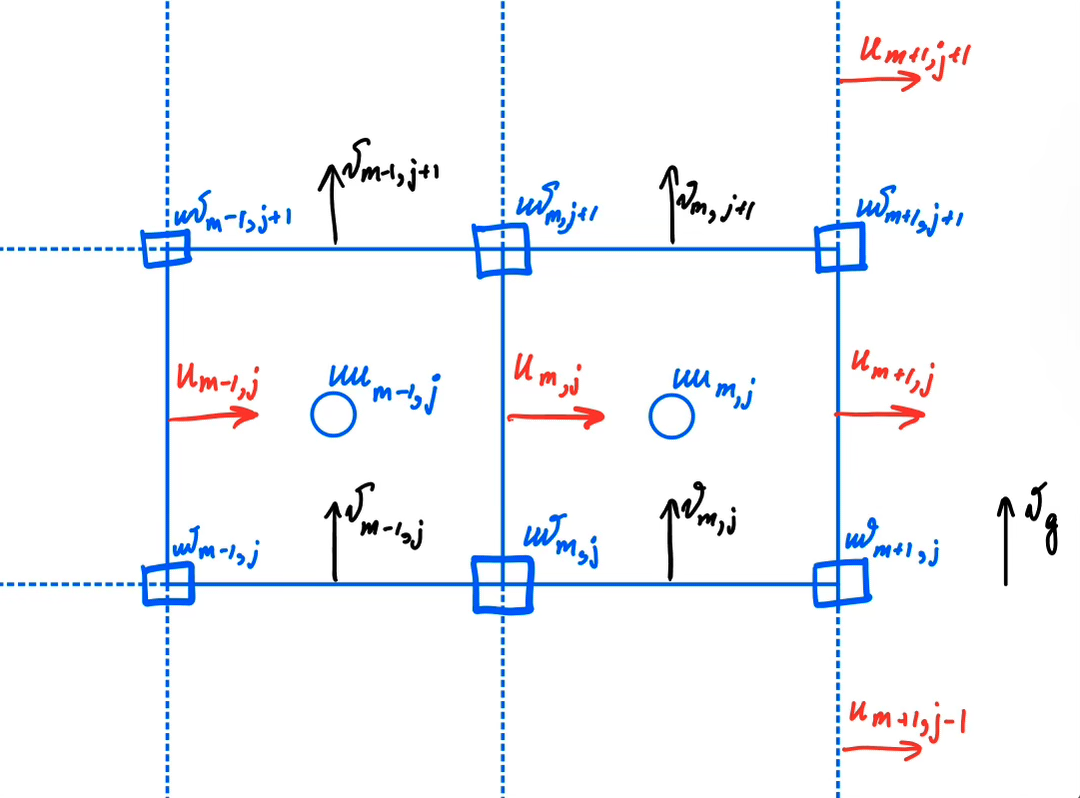
\includegraphics[width=0.45\paperwidth]{ADV-right}
  }
  \caption{$\hat{L}^u_{xx},\hat{L}^v_{xx}$ at the right boundary.}\label{fig:luxx-right}
\end{figure}
The last unknown element of \cref{eqn:NSE-dsm-bl-system-schemes} in $x$ direction is $u^{n+1}_{M-\frac{1}{2},j}$ on \cref{fig:luxx-right}. To apply \cref{eqn:laplacian-discretization-non-uniform-dx} we need to express $u^{n+1}_{M+\frac{1}{2},j}$ using \cref{eqn:jin-bc-transient}.
\begin{equation*}
\begin{gathered}
\frac{{u}^{n+1}_{M+\frac{1}{2},j}-{u}^n_{M+\frac{1}{2},j}}{\Delta t}
+\frac{u^n_{M+\frac{1}{2},j}}{2}
\left[
\left(
	\frac{u^{n+1}_{M+\frac{1}{2},j}-u^{n+1}_{M-\frac{1}{2},j}}{\Delta x_M}
\right)
+\left(
	\frac{u^{n}_{M+\frac{1}{2},j}-u^{n}_{M-\frac{1}{2},j}}{\Delta x_M}
\right)
\right] =\\
=\nu\left(\frac{1}{h_c h_s}u^{n}_{M+\frac{1}{2},j-1} - \frac{2}{h_n h_s}u^{n}_{M+\frac{1}{2},j} + \frac{1}{h_c h_n}u^n_{M+\frac{1}{2},j+1}\right)
\end{gathered}
\end{equation*}
leads to %%%%%%%%%%%%%%%%%
\begin{equation}\label[bc]{eqn:bc-u-right-long}
\begin{gathered}
\left(\frac{1}{\Delta t} + \frac{u^n_{M+\frac{1}{2},j}}{2\Delta x_M}\right){{u}^{n+1}_{M+\frac{1}{2},j}}
=
u^{n+1}_{M-\frac{1}{2},j}\frac{u^n_{M+\frac{1}{2},j}}{2\Delta x_M}-\\
-\frac{u^n_{M+\frac{1}{2},j}}{2}\frac{u^{n}_{M+\frac{1}{2},j}-u^{n}_{M-\frac{1}{2},j}}{\Delta x_M}
+\frac{{u}^n_{M+\frac{1}{2},j}}{\Delta t}
+\nu\left(\frac{1}{h_c h_s}u^{n}_{M+\frac{1}{2},j-1} - \frac{2}{h_n h_s}u^{n}_{M+\frac{1}{2},j} + \frac{1}{h_c h_n}u^n_{M+\frac{1}{2},j+1}\right).
\end{gathered}
\end{equation}
Note that $\left(\frac{1}{\Delta t} + \frac{u^n_{M+\frac{1}{2},j}}{2\Delta x_M}\right)$ can be made to never be zero regardless of the flow direction, hence dividing by it is allowed. The second line of fully discretized \cref{eqn:bc-u-right-long} is treated explicitly since we posses the flow data at time steps $n$ and earlier. Denote explicit terms as
\begin{equation*}
	bc_{u-\text{explicit}}^n=-\frac{u^n_{M+\frac{1}{2},j}}{2}\frac{u^{n}_{M+\frac{1}{2},j}-u^{n}_{M-\frac{1}{2},j}}{\Delta x_M}
+\frac{{u}^n_{M+\frac{1}{2},j}}{\Delta t}
+\nu\left(\frac{1}{h_c h_s}u^{n}_{M+\frac{1}{2},j-1} - \frac{2}{h_n h_s}u^{n}_{M+\frac{1}{2},j} + \frac{1}{h_c h_n}u^n_{M+\frac{1}{2},j+1}\right),
\end{equation*}
which simplifies \cref{eqn:bc-u-right-long} to 
\begin{equation}\label[bc]{eqn:bc-u-right}
\begin{gathered}
\left(\frac{1}{\Delta t} + \frac{u^n_{M+\frac{1}{2},j}}{2\Delta x_M}\right){{u}^{n+1}_{M+\frac{1}{2},j}}
=
u^{n+1}_{M-\frac{1}{2},j}\frac{u^n_{M+\frac{1}{2},j}}{2\Delta x_M}+bc_{u-\text{explicit}}^n.
\end{gathered}
\end{equation}

Next, we plug \cref{eqn:bc-u-right} into \cref{eqn:laplacian-discretization-non-uniform-dx}, which finally leads us to
\begin{equation}\label{eqn:luxx-right}
\begin{aligned}
	\left.\frac{\partial ^2 u}{\partial x^2}\right|_{M-\frac{1}{2},j}^{n+1}
	&=\frac{1}{h_c h_e}u^{n+1}_{M+\frac{1}{2},j} - \frac{2}{h_w h_e}u^{n+1}_{M-\frac{1}{2},j} + \frac{1}{h_c h_w}u^{n+1}_{M-\frac{1}{2}-1,j}+h.o.t.\\
	&=\frac{1}{h_c h_e}\frac{\left.u^{n+1}_{M-\frac{1}{2},j}\frac{u^n_{M+\frac{1}{2},j}}{2h_e}+bc_{u-\text{explicit}}^n\right.}{\left.\frac{1}{\Delta t} + \frac{u^n_{M+\frac{1}{2},j}}{2\Delta x_M}\right.}- \frac{2}{h_w h_e}u^{n+1}_{M-\frac{1}{2},j} + \frac{1}{h_c h_w}u^{n+1}_{M-\frac{1}{2}-1,j}+h.o.t.\\
	&=\left[ \frac{1}{h_c h_e}\left(\frac{u^n_{M+\frac{1}{2},j}}{2h_e\left[\frac{1}{\Delta t} + \frac{u^n_{M+\frac{1}{2},j}}{2\Delta x_M}\right]} \right) -\frac{2}{h_w h_e}\right]u^{n+1}_{M-\frac{1}{2},j} + \frac{1}{h_c h_w}u^{n+1}_{M-\frac{1}{2}-1,j} + \frac{bc_{u-\text{explicit}}^n}{h_c h_e\left(\frac{1}{\Delta t} + \frac{u^n_{M+\frac{1}{2},j}}{2\Delta x_M}\right)}+h.o.t..
\end{aligned}
\end{equation}

Condition for $v$ component is not as trivial as for $u$ since there is no $v$ directly at the boundary due to the staggered grid arrangement. We need to express $v_g=v_{M+1,j-\frac{1}{2}}$ in terms of the right-most unknown $v_{M,j-\frac{1}{2}}$ component for the diffusion operator. 
We can use more than one value of $v$ from inner part of the domain to express the ghost velocity outside. However, this will lead to change of non-diagonal elements in diffusion operator, which will cause Laplacian matrix to be asymmetric. Therefore, we are restricted to use the elements of the main diagonal to express the ghost velocities outside the computational domain. Hence, interpolation leads to
\begin{equation*}
	v_{\text{BC}}=v_{M+\frac{1}{2},j-\frac{1}{2}}=\frac{v_{M+1,j-\frac{1}{2}}+v_{M,j-\frac{1}{2}}}{2},
\end{equation*}
where $v_{M+1,j-\frac{1}{2}}$ is ghost component outside the domain. It is also possible to apply central difference to the advection terms at the boundary $\left( \frac{\partial v}{\partial x}\right)_{M+\frac{1}{2},j-\frac{1}{2}}=\frac{v_{M+1,j-\frac{1}{2}}-v_{M,j-\frac{1}{2}}}{\Delta x_{M+\frac{1}{2}}}$.

\cref{eqn:jin-bc-transient} using the approximations from above can be rewritten for $v_{M+\frac{1}{2},j-\frac{1}{2}}$ component at the boundary as
\begin{equation*}
\begin{gathered}
\frac{{\left( \frac{v^{n+1}_{M+1,j-\frac{1}{2}}+v^{n+1}_{M,j-\frac{1}{2}}}{2}\right)}-\left( \frac{v^n_{M+1,j-\frac{1}{2}}+v^n_{M,j-\frac{1}{2}}}{2} \right) }{\Delta t}+\\
+\frac{\left.u^n_{M+\frac{1}{2},j-\frac{1}{2}}\right.}{2}
\left[
\left(
	\frac{v^{n+1}_{M+1,j-\frac{1}{2}}-v^{n+1}_{M,j-\frac{1}{2}}}{\Delta x_{M+\frac{1}{2}}}
\right) \right.
+\left.\left(
	\frac{v^{n}_{M+1,j-\frac{1}{2}}-v^{n}_{M,j-\frac{1}{2}}}{\Delta x_{M+\frac{1}{2}}}
\right)
\right]= \\
=\nu\left[\frac{1}{h_c h_s}\left(\frac{v^{n}_{M+1,j-\frac{1}{2}-1}+v^{n}_{M,j-\frac{1}{2}-1}}{2} \right) - \frac{2}{h_n h_s}\left(\frac{v^{n}_{M+1,j-\frac{1}{2}}+v^{n}_{M,j-\frac{1}{2}}}{2} \right) + \frac{1}{h_c h_n}\left(\frac{v^{n}_{M+1,j+\frac{1}{2}}+v^{n}_{M,j+\frac{1}{2}}}{2} \right)\right],
\end{gathered}
\end{equation*}
which is used to express ghost velocity $v^{n+1}_{M+1,j-\frac{1}{2}}$ after rearranging
\begin{equation}\label[bc]{eqn:bc-v-right-long}
\begin{gathered}
\left( \frac{1}{2\Delta t} + \frac{u^n_{M+\frac{1}{2},j-\frac{1}{2}}}{2\Delta x_{M+\frac{1}{2}}}\right) v^{n+1}_{M+1,j-\frac{1}{2}}
=\left( -\frac{1}{2\Delta t}+\frac{u^n_{M+\frac{1}{2},j-\frac{1}{2}}}{2\Delta x_{M+\frac{1}{2}}} \right)v^{n+1}_{M,j-\frac{1}{2}}+\\
+\left( \frac{v^n_{M+1,j-\frac{1}{2}}+v^n_{M,j-\frac{1}{2}}}{2\Delta t} \right)
+ \frac{\left.u^n_{M+\frac{1}{2},j-\frac{1}{2}}\right.}{2}\left(\frac{v^{n}_{M+1,j-\frac{1}{2}}-v^{n}_{M,j-\frac{1}{2}}}{\Delta x_{M+\frac{1}{2}}}\right)+\\
+\nu\left[\frac{1}{h_c h_s}\left(\frac{v^{n}_{M+1,j-\frac{1}{2}-1}+v^{n}_{M,j-\frac{1}{2}-1}}{2} \right) - \frac{2}{h_n h_s}\left(\frac{v^{n}_{M+1,j-\frac{1}{2}}+v^{n}_{M,j-\frac{1}{2}}}{2} \right) + \frac{1}{h_c h_n}\left(\frac{v^{n}_{M+1,j+\frac{1}{2}}+v^{n}_{M,j+\frac{1}{2}}}{2} \right)\right].
\end{gathered}
\end{equation}
Let us denote explicit terms from last two rows as
\begin{equation*}
\begin{gathered}
	bc_{v-\text{explicit}}^n=\left( \frac{v^n_{M+1,j-\frac{1}{2}}+v^n_{M,j-\frac{1}{2}}}{2\Delta t} \right)
+ \frac{\left.u^n_{M+\frac{1}{2},j-\frac{1}{2}}\right.}{2}\left(\frac{v^{n}_{M+1,j-\frac{1}{2}}-v^{n}_{M,j-\frac{1}{2}}}{\Delta x_{M+\frac{1}{2}}}\right)+\\
+\nu\left[\frac{1}{h_c h_s}\left(\frac{v^{n}_{M+1,j-\frac{1}{2}-1}+v^{n}_{M,j-\frac{1}{2}-1}}{2} \right) - \frac{2}{h_n h_s}\left(\frac{v^{n}_{M+1,j-\frac{1}{2}}+v^{n}_{M,j-\frac{1}{2}}}{2} \right) + \frac{1}{h_c h_n}\left(\frac{v^{n}_{M+1,j+\frac{1}{2}}+v^{n}_{M,j+\frac{1}{2}}}{2} \right)\right].
\end{gathered}
\end{equation*}
Then \cref{eqn:bc-v-right-long} simplifies to
\begin{equation}\label[bc]{eqn:bc-v-right}
\begin{gathered}
\left( \frac{1}{2\Delta t} + \frac{u^n_{M+\frac{1}{2},j-\frac{1}{2}}}{2\Delta x_{M+\frac{1}{2}}}\right) v^{n+1}_{M+1,j-\frac{1}{2}}
=\left( -\frac{1}{2\Delta t}+\frac{u^n_{M+\frac{1}{2},j-\frac{1}{2}}}{2\Delta x_{M+\frac{1}{2}}} \right)v^{n+1}_{M,j-\frac{1}{2}}+bc_{v-\text{explicit}}^n.
\end{gathered}
\end{equation}

The ultimate step is to plug \cref{eqn:bc-v-right} into \cref{eqn:laplacian-discretization-non-uniform-dx} which will result in diffusion approximation of $v$ in $x$ direction of the right-most unknown component
\begin{equation}\label{{eqn:lvxx-right}}
\begin{aligned}
	\left.\frac{\partial ^2 v}{\partial x^2}\right|_{M,j-\frac{1}{2}}^{n+1}
	&=\frac{1}{h_c h_e}v^{n+1}_{M+1,j-\frac{1}{2}} - \frac{2}{h_w h_e}v^{n+1}_{M,j-\frac{1}{2}} + \frac{1}{h_c h_w}v^{n+1}_{M-1,j-\frac{1}{2}}+h.o.t.\\
	&=\frac{1}{h_c h_e}\left[\frac{\left( -\frac{1}{2\Delta t}+\frac{u^n_{M+\frac{1}{2},j-\frac{1}{2}}}{2h_e} \right)v^{n+1}_{M,j-\frac{1}{2}}+bc_{v-\text{explicit}}^n}{\left. \frac{1}{2\Delta t} + \frac{u^n_{M+\frac{1}{2},j-\frac{1}{2}}}{2h_e}\right.}\right]- \frac{2}{h_w h_e}v^{n+1}_{M,j-\frac{1}{2}} + \frac{1}{h_c h_w}v^{n+1}_{M-1,j-\frac{1}{2}}+h.o.t.\\
	&=\left[ \frac{1}{h_c h_e}\left(\frac{\left. -\frac{1}{2\Delta t}+\frac{u^n_{M+\frac{1}{2},j-\frac{1}{2}}}{2h_e} \right.}{\left. \frac{1}{2\Delta t} + \frac{u^n_{M+\frac{1}{2},j-\frac{1}{2}}}{2h_e}\right.} \right) -\frac{2}{h_w h_e}\right]v^{n+1}_{M,j-\frac{1}{2}} + \frac{1}{h_c h_w}v^{n+1}_{M-1,j-\frac{1}{2}} + \frac{bc_{v-\text{explicit}}^n}{h_c h_e\left( \frac{1}{2\Delta t} + \frac{u^n_{M+\frac{1}{2},j-\frac{1}{2}}}{2h_e}\right)}+h.o.t..
\end{aligned}
\end{equation}

Let us now try to apply \cref{eqn:jin-bc-transient-consistent} which is consistent with schemes for the inner part to the boundary values at the outlet
\begin{equation*}
\begin{gathered}
\frac{{u}^{n+1}_{M+\frac{1}{2},j}-{u}_{M+\frac{1}{2},j}^n}{\Delta t}+\left[\frac{3}{2}{u_{M+\frac{1}{2},j}^n}\left(\frac{\partial {u}}{\partial x}\right)^{n}_{M+\frac{1}{2},j}-\frac{1}{2}{u_{M+\frac{1}{2},j}^{n-1}}\left(\frac{\partial {u}}{\partial x}\right)^{n-1}_{M+\frac{1}{2},j}\right]\\
=\nu\left[\left(\frac{\partial^2 {u}}{\partial y^2}\right)^{n+1}_{M+\frac{1}{2},j}+\left(\frac{\partial^2 {u}}{\partial y^2}\right)^{n}_{M+\frac{1}{2},j}\right].
\end{gathered}
\end{equation*}
The above equation after discretizing spatially becomes
\begin{equation}\label[bc]{eqn:jin-bc-full-consistent}
\begin{gathered}
\frac{\nu}{h_c h_n}u^{n+1}_{M+\frac{1}{2},j+1} - \left(\frac{2\nu}{h_s h_n}-\frac{1}{\Delta t}\right)u^{n+1}_{M+\frac{1}{2},j} + \frac{\nu}{h_c h_s}u^{n+1}_{M+\frac{1}{2},j-1}\\
=-\frac{{u}_{M+\frac{1}{2},j}^n}{\Delta t}+\left[\frac{3}{2}{u_{M+\frac{1}{2},j}^n}\left(\frac{u_{M+\frac{1}{2},j}^n-u_{M-\frac{1}{2},j}^n}{\Delta x_M}\right)-\frac{1}{2}{u_{M+\frac{1}{2},j}^{n-1}}\left(\frac{u_{M+\frac{1}{2},j}^{n-1}-u_{M-\frac{1}{2},j}^{n-1}}{\Delta x_M}\right)\right]\\
-\left[\frac{\nu}{h_c h_n}u^{n}_{M+\frac{1}{2},j+1}-\frac{2\nu}{h_s h_n}u^{n}_{M+\frac{1}{2},j} + \frac{\nu}{h_c h_s}u^{n}_{M+\frac{1}{2},j-1}\right].
\end{gathered}
\end{equation}

The fully discretized \cref{eqn:jin-bc-full-consistent} from above is a system of linear equations at time step $n+1$ and only has to be solved for the outlet boundary values of $u$. We know both topmost velocity $u_{\text{top}}=u_{\text{freestream}}$ and bottommost $u_{\text{bot}}=u_{\text{wall}}$ which play roles of boundary values for this system of equations. However, there is an issue that no velocity values at time step $n+1$ are passed from the inner part of the domain, the whole equation is self-sufficient and takes only the inner data from previous time steps $n$ and $n-1$.

\textbf{Left boundary.} 
The exact value on the left boundary ($u_{\frac{1}{2},j}$ in a box on \cref{fig:luxx-left}) is given as a Dirichlet boundary condition, hence, it is possible to move the corresponding terms together with the coefficients to the right-hand side of the linear system and treat the values explicitly. The values are moved to the vector $\hat{bc}_1$ on the right-hand side of \cref{eqn:NSE-dsm-bl-system-schemes}.
\begin{figure}[H] % here, bottom, top
  \centering{
  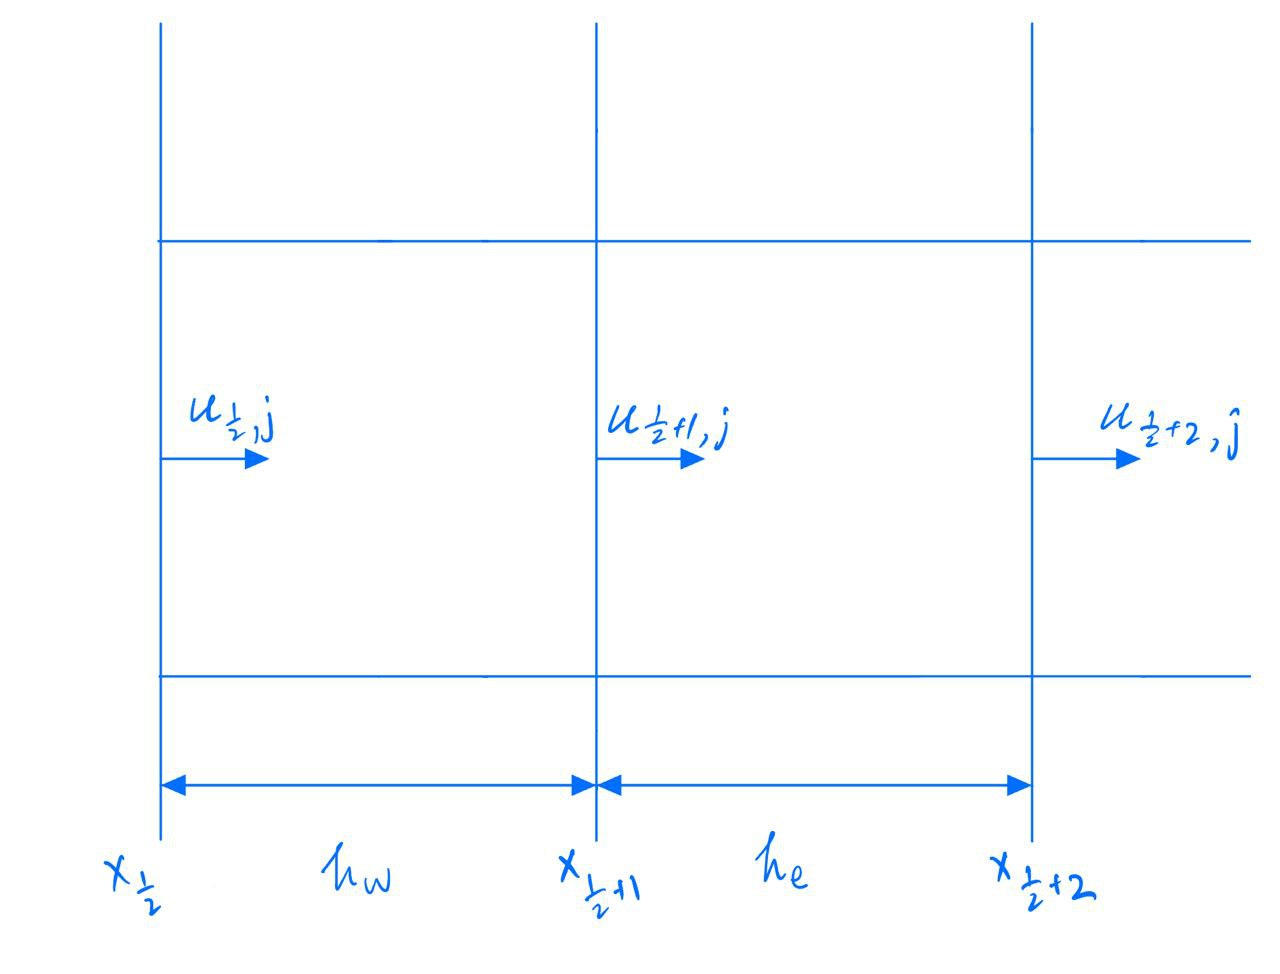
\includegraphics[width=0.55\paperwidth]{Luxx-left}
  }
  \caption{$\hat{L}^u_{xx}$ at the left boundary.}\label{fig:luxx-left}
\end{figure}

\textbf{Top boundary.} Most of the flow that differs much from the freestream is likely to happen closer to the wall, thus, we can incorporate symmetric boundary conditions over the top. \cref{eqn:symmetric-bc} leads to $v_{\text{top}}=0, u_{\text{top}}=u_{\text{freestream}}$, which affects only the $\hat{L}^u_{yy}$ and $\hat{L}^v_{yy}$ due to the 5-point stencil discretization. We will focus on $\hat{L}^u_{yy}$ in this part; $\hat{L}^v_{yy}$ is computed in a similar manner. 

\begin{figure}[h]
\centering{
  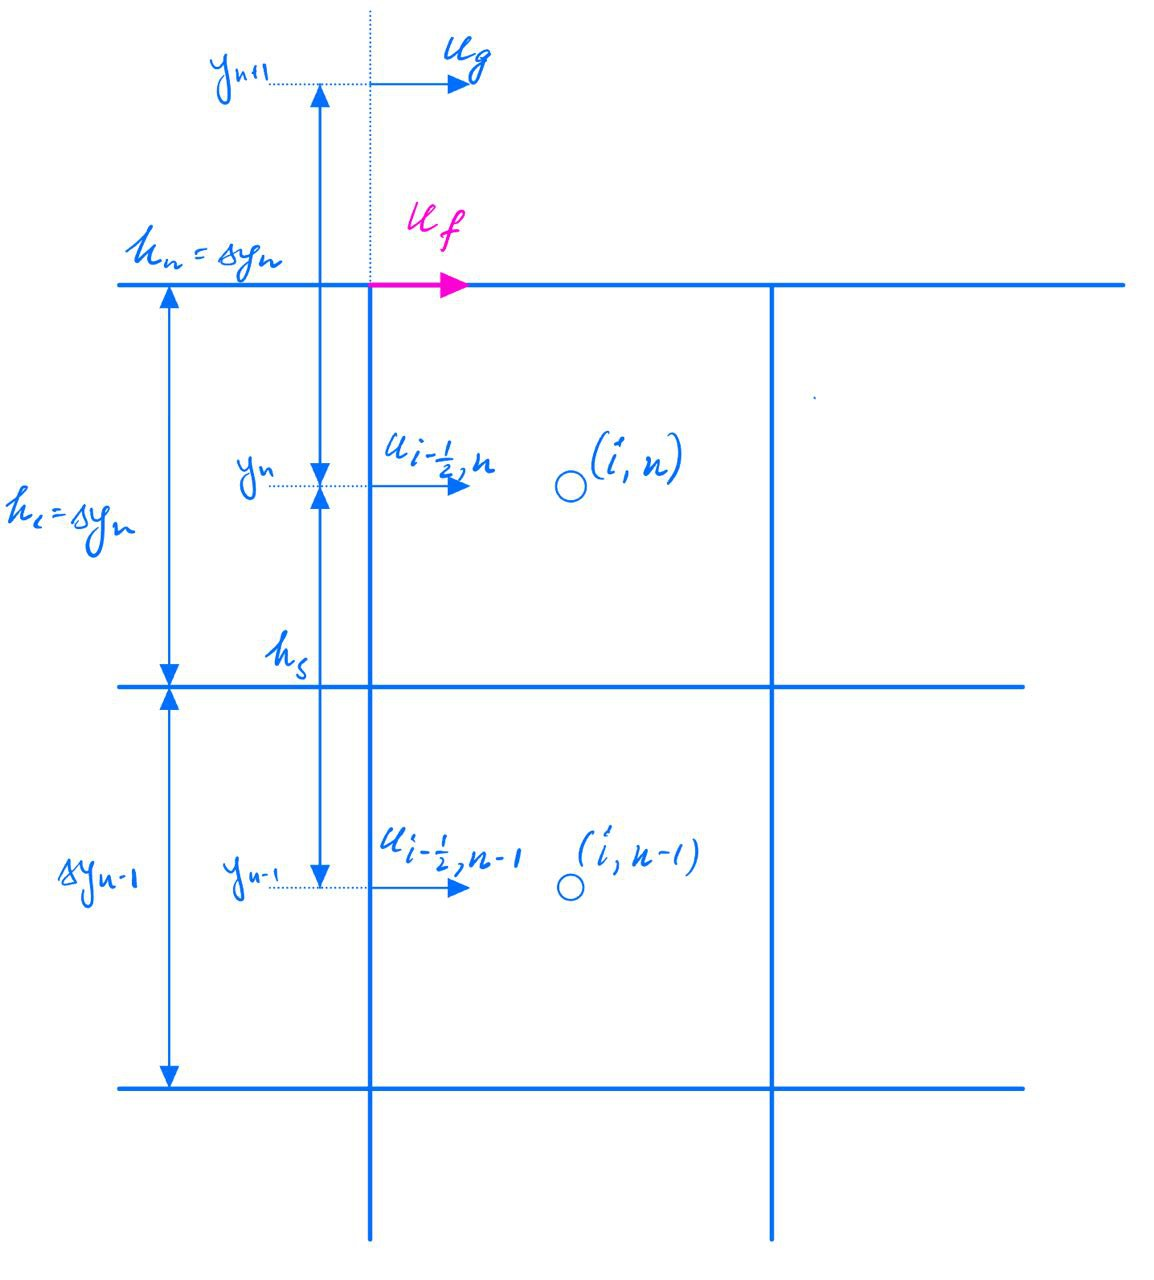
\includegraphics[width=0.45\paperwidth]{Luxx-top.jpg}
  }
  \caption{$\hat{L}^u_{yy}$ at top boundary.}\label{fig:luxx-top}
\end{figure}

Consider the neighbouring cells near the wall as in \cref{fig:luxx-top}. Resultant \cref{eqn:laplacian-discretization-non-uniform-dx}  can be written as
\begin{equation}\label{eqn:laplacian-discretization-non-uniform-dy}
\left.\frac{\partial^2 u}{\partial y^2}\right|_{i-\frac{1}{2},N}=\frac{u_g\left(h_s\right)+u_{i-\frac{1}{2},N}\left(-2 h_c\right)+u_{i-\frac{1}{2},N-1}\left(h_n\right)}{h_n h_s h_c},
\end{equation}
where $h_s=y_{n}-y_{n-1}, h_n = y_{n+1}-y_n, h_c = \frac{y_{n+1}-y_{n-1}}{2}=\frac{h_s+h_n}{2}$.

It is possible to make the order of the scheme $O(\Delta y^2)$ near the boundary as per \cref{eqn:laplacian-discretization-non-uniform-dx} if $u_g$ and $u_{i-\frac{1}{2},N-1}$ are set to be equidistant from $u_{i-\frac{1}{2},N}$.The value of $u$ along the top face is known to be freestream velocity $u_{{f}}$, interpolation of freestream velocity $u_{f} = \frac{u_g+u_{i-\frac{1}{2},N}}{2}\implies u_g=2u_{f}-u_{i-\frac{1}{2},N}$, which we can plug into \cref{eqn:laplacian-discretization-non-uniform-dy} from above to obtain
\begin{equation}
\begin{aligned}
& \left.\frac{\partial ^2 u}{\partial y^2}\right|_{i-\frac{1}{2},N}=\frac{2 u_f h_s}{h_n h_s h_c}+u_{i-\frac{1}{2},N}\left(\frac{-h_s}{h_n h_s h_c}+\frac{-2 h_c}{h_n h_s h_c}\right)+u_{i-\frac{1}{2},N-1} \frac{h_n}{u_c h_s h},\\
& \left.\frac{\partial^2 u}{\partial y^2}\right|_{i-\frac{1}{2},N}=\frac{2 u_f}{h_c h_c}+u_{i-\frac{1}{2},N}\left(\frac{-\left(2 h_c+h_s\right)}{h_c h_s h_c}\right)+u_{i-\frac{1}{2},N-1} \frac{1}{h_s h_c}, \\
& \left.\frac{\partial^2 u}{\partial y^2}\right|_{i-\frac{1}{2},N}=\frac{2 u_f}{h_c{ }^2}+u_{i-\frac{1}{2},N}\left(\frac{-\left(2 h_c+h_s\right)}{h_c^2 h_s}\right)+u_{i-\frac{1}{2},N-1} \frac{1}{h_s h_c}.
\end{aligned}
\end{equation}

The first summand from the above equation is treated explicitly, i.e. moved to the vector $\hat{bc}_1$ on the right-hand side in \cref{eqn:NSE-dsm-bl-system-schemes}, while the other two coefficients are used as elements for the $\hat{L}^u_{yy}$ matrix.

\textbf{Bottom boundary.}
It is, in fact, possible to directly use the third velocity directly from the boundary. However, the order of such a scheme will then be reduced due to the large ratio of the distances between the neighbouring velocities. If, on the other hand, we introduce a ghost velocity $u_g$, we have the freedom of where to place it. Let us use \cref{eqn:laplacian-discretization-non-uniform-dx} and change the distances between velocities as in \cref{fig:luxx-bottom}, which leads to
\begin{equation}
\begin{aligned}
&\left.\frac{\partial^ 2 u}{\partial y^2}\right|_{i-\frac{1}{2},1}=u_{i-\frac{1}{2},2}\left(\frac{1}{h_n h_c}\right)+u_{i-\frac{1}{2},1}\left(\frac{-2}{h_n h_s}\right)+u_g\left(\frac{1}{h_s h_c}\right).\\
\end{aligned}
\end{equation}

\begin{figure}[H] % here, bottom, top
  \centering{
  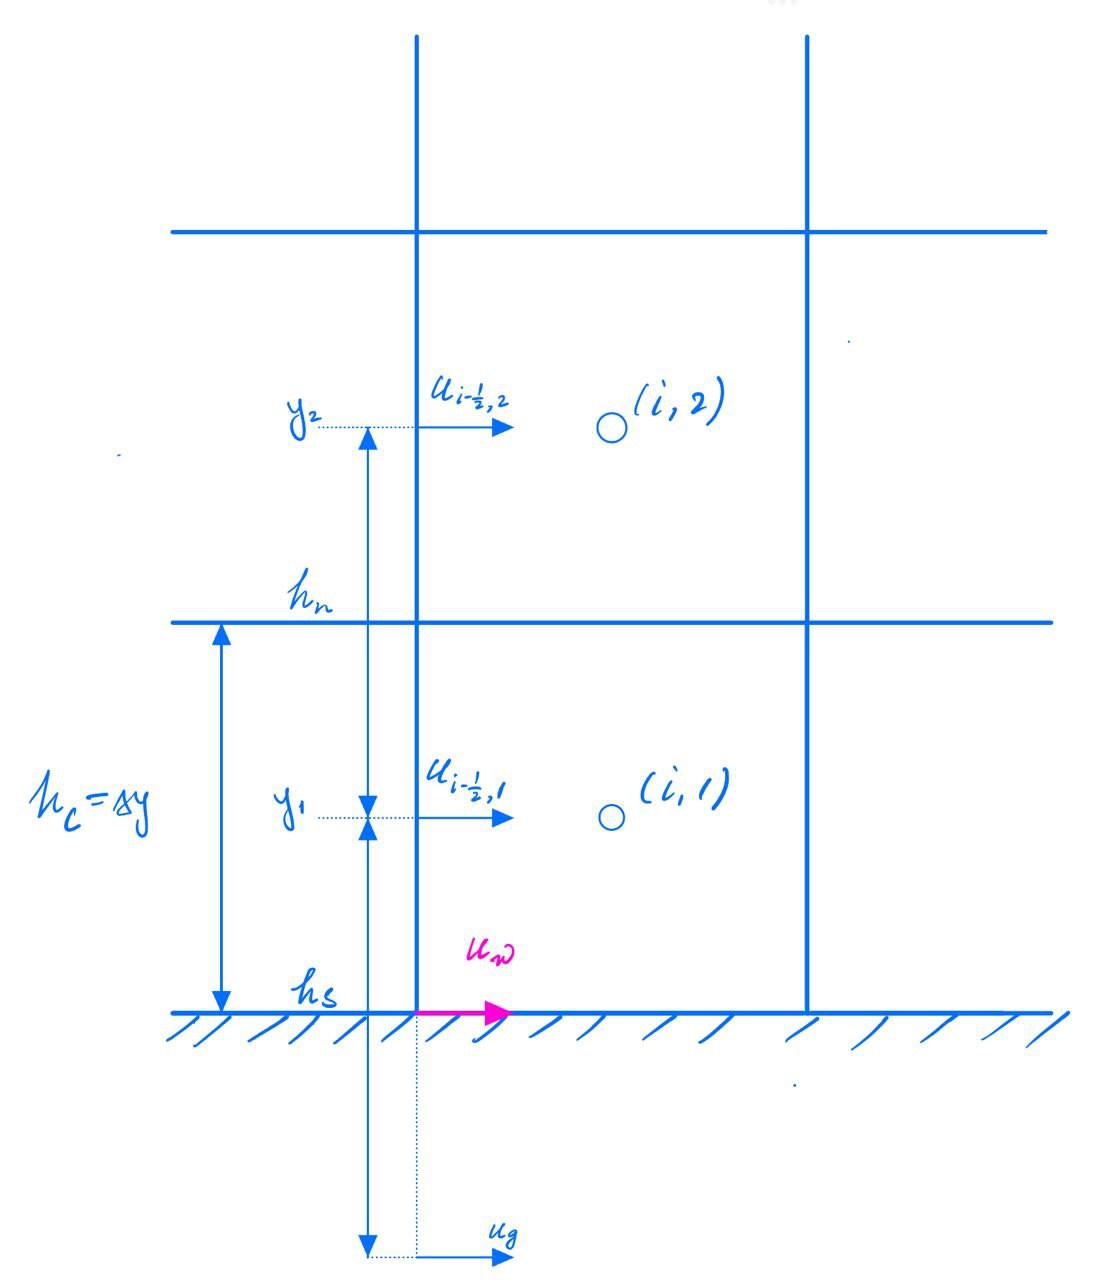
\includegraphics[width=0.45\paperwidth]{Luxx-bottom}
  }
  \caption{$\hat{L}^u_{yy}$ at the bottom boundary.}\label{fig:luxx-bottom}
\end{figure}

The position of $u_g$ is not fixed, we can make the order of the scheme $O(\Delta y^2)$ if $h_s=h_n$. Interpolation of velocity at the wall $u_{w} =\frac{u_{i-\frac{1}{2},1}+u_g}{2}=0 \Rightarrow u_g=-2 u_{i-\frac{1}{2},1}$, then
\begin{equation}\label{eqn:luxx-bot}
\begin{aligned}
\left.\frac{\partial^2 u}{\partial y^2}\right|_{i-\frac{1}{2},1} 
& =u_{i-\frac{1}{2},2}\left(\frac{1}{h_n h_c}\right)+u_{i-\frac{1}{2},1}\left(\frac{-2}{h_n h_s}+\frac{-2}{h_s h_c}\right) \\
& =u_{i-\frac{1}{2},2}\left(\frac{1}{h_n h_c}\right)+u_{i-\frac{1}{2},1}\left(\frac{-2 h_c-2 h_n}{h_s h_c h_n}\right).
\end{aligned}
\end{equation}
The coefficients from \cref{eqn:luxx-bot} are distributed into the $\hat{L}^u_{yy}$ matrix similarly to previous boundary cases.


%%%%%%%%%%%%%%%%%%%%%%%%%%%%%%%%%%%%%%%%%%%%%%
\subsubsection{Divergence}\label{subsec:divergence}

One of the advantages of the staggered grid is that the discrete divergence $D$ and gradient $G$ operators are equal to the negative transpose of each other. 
%Our goal is to eliminate the pressure from the system, \cref{sec:nullspace-method} will explain the use of this property in detail. 
In this section we will show one side of why this identity is true, the other part could be found in \cref{subsec:gradient}.
The second line of \cref{eqn:nse-matrix} reads
\begin{equation*}
\begin{gathered}
\hat{D}\boldsymbol{v}=\hat{bc}_2,\\
\left[ 
\begin{array}{ll}
\hat{D}_x & \hat{D}_y 	
\end{array}
\right]\left[\begin{array}{l}
u\\
v
\end{array}
\right]=\hat{bc}_2
, \\
\frac{1}{\Delta x} D_x u+\frac{1}{\Delta y} D_y v=\hat{bc}_2, \\
\frac{1}{\Delta _{xy}}\left[\begin{array}{ll}
D_x & D_y
\end{array}\right]\left[\begin{array}{l}
u \Delta y \\
v \Delta x
\end{array}\right]=\frac{1}{\Delta _{xy}} D q=\hat{bc}_2,
\end{gathered}
\end{equation*}
where vector $q$ is referred to as velocity flux, and the matrix $D=[D_x D_y]$ without hat is the divergence matrix of integer coefficients. Matrix
\begin{equation}\label{eqn:delta-xy}
	\Delta _{xy}=
	\begin{bmatrix}{}
		\frac{1}{\Delta x_1\Delta y_1}		&0	&\dots	&0\\
		0		&\frac{1}{\Delta x_2\Delta y_1}	&\dots	&0\\
		\vdots		&\vdots	&\ddots	&\vdots\\
		0		&0	&\dots	&\frac{1}{\Delta x_M\Delta y_N}
	\end{bmatrix}
\end{equation}
is $MN\times MN$ diagonal matrix with entries corresponding to the inverse volumes of cells. 

The second-order central difference scheme was employed in the construction of $D$, the order is consistent with the other spatial schemes. Consider a finite volume $V_{i,j}$, continuity equation for the cell centre is then expressed as
\begin{equation*}
	\left(\frac{\partial u}{\partial x} + \frac{\partial v}{\partial y}\right)_{i,j}=0,
\end{equation*}
which can be discretized at cell centre $i,j$ using central difference schemes into
\begin{equation*}
  \frac{u_{i+\frac{1}{2},j} - u_{i-\frac{1}{2},j}}{\Delta x_i}+  \frac{v_{i,j+\frac{1}{2}} - v_{i,j-\frac{1}{2}}}{\Delta y_j}=0.
\end{equation*}

\begin{figure}[H] % here, bottom, top
  \centering{
  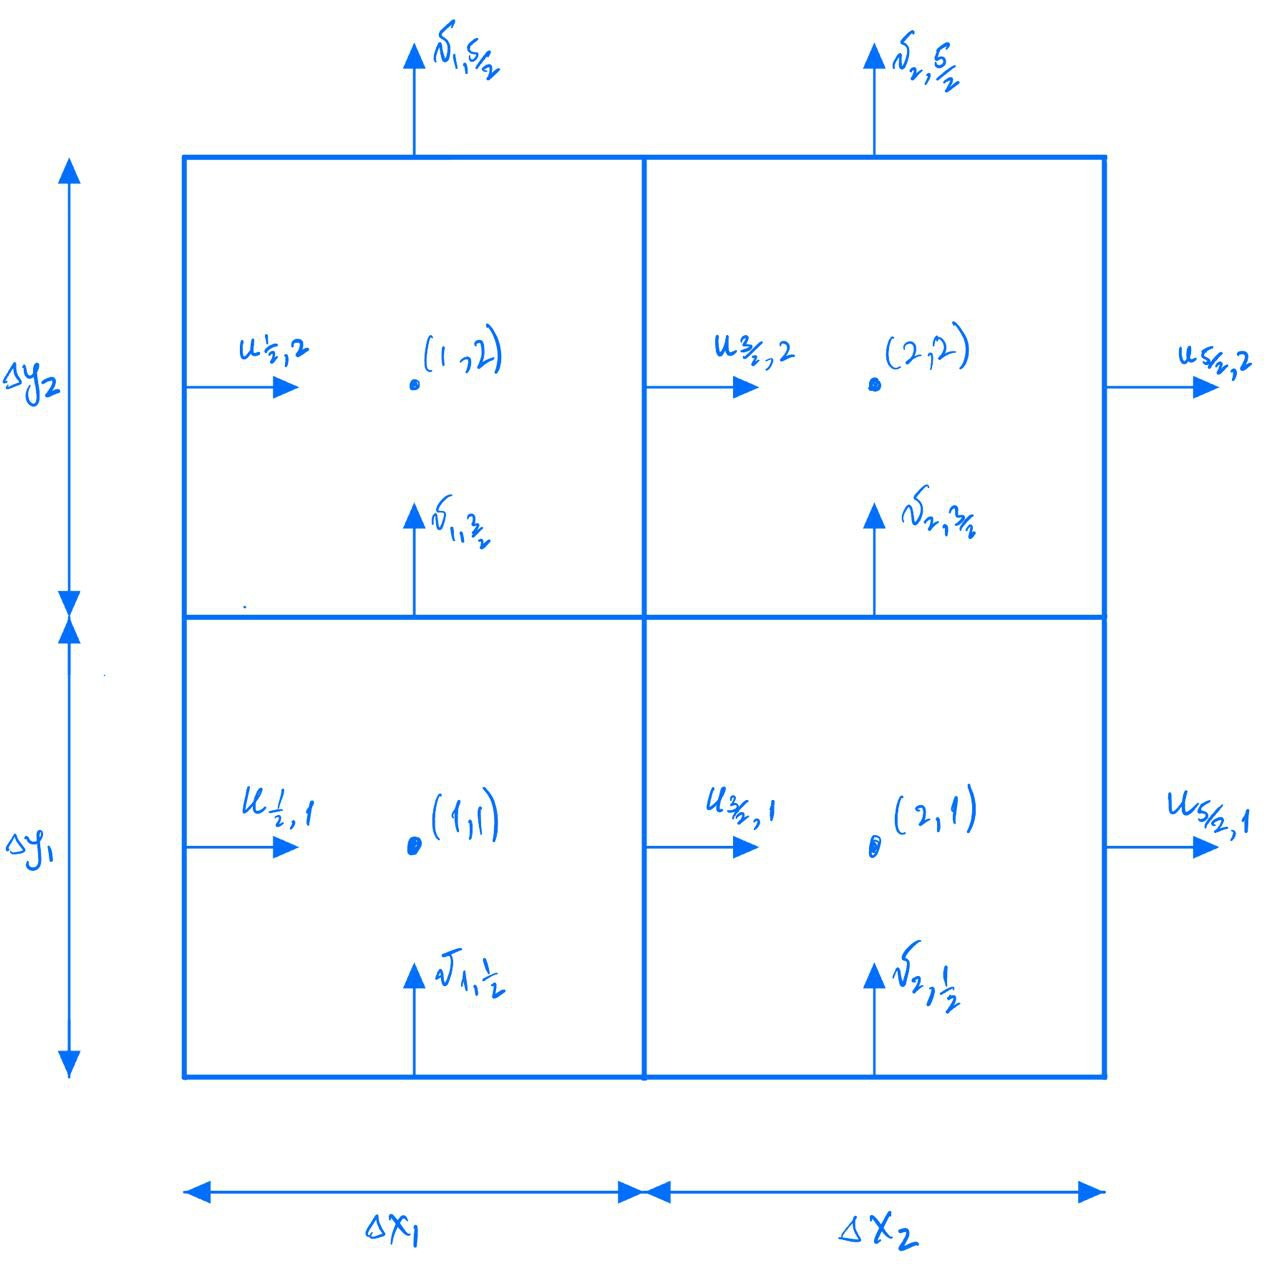
\includegraphics[width=0.45\paperwidth]{D-example-2x2}
  }
  \caption{$2\times 2$ grid example for divergence operator.}\label{fig:D-example-2x2}
\end{figure}

To provide a good visual example, consider $2 \times 2$ grid as in \cref{fig:D-example-2x2} with the same boundary conditions as in \cref{eqs:NSE-dsm-bl}. The partial derivatives of divergence operator evaluated at cell centres are: 
%\begin{equation}
%  \frac{1}{\Delta x_i \Delta y_i}\left[1\quad -1\quad1\quad-1\right] \left[\Delta y_i u_{i+1,j}, \Delta y_i  u_{i,j}, \Delta x_i v_{i,j+1}, \Delta x_i v_{i,j}\right]^T=0.
%\end{equation}
\begin{alignat*}{2}
	V_{1,1}:\frac{u_{\frac{3}{2},1} - u_{\frac{1}{2},1}}{\Delta x_1}+\frac{v_{1,\frac{3}{2}} - v_{1,\frac{1}{2}}}{\Delta y_1}=0,\\
	V_{2,1}: \frac{u_{\frac{5}{2},1} - u_{\frac{3}{2},1}}{\Delta x_2}+\frac{v_{2,\frac{3}{2}} - v_{2,\frac{1}{2}}}{\Delta y_1}=0,\\
	V_{1,2}:\frac{u_{\frac{3}{2},2} - u_{\frac{1}{2},2}}{\Delta x_1}+\frac{v_{1,\frac{5}{2}} - v_{1,\frac{3}{2}}}{\Delta y_2}=0,\\
	V_{2,2}:\frac{u_{\frac{5}{2},2} - u_{\frac{3}{2},2}}{\Delta x_2}+\frac{v_{2,\frac{5}{2}} - v_{2,\frac{3}{2}}}{\Delta y_2}=0.
\end{alignat*}

%\begin{enumerate}
%	\item[$V_{1,1}$]: $\frac{u_{1,2} - u_{1,1}}{\Delta x_1}+\frac{v_{2,1} - v_{1,1}}{\Delta y_1}=0$.
%	\item[$V_{1,2}$]: $\frac{u_{1,3} - u_{1,2}}{\Delta x_2}+\frac{v_{2,2} - v_{1,2}}{\Delta y_1}=0$.
%	\item[$V_{2,1}$]: $\frac{u_{2,2} - u_{2,1}}{\Delta x_1}+\frac{v_{3,1} - v_{2,1}}{\Delta y_2}=0$.
%	\item[$V_{2,2}$]: $\frac{u_{2,3} - u_{2,2}}{\Delta x_2}+\frac{v_{3,2} - v_{2,2}}{\Delta y_2}=0$.
%\end{enumerate}

After applying the boundary conditions to the above equations, we obtain the system
\begin{equation}\label[system]{eqn:divergence-matrix}
	\begin{bmatrix}{}
		\frac{1}{\Delta x_1\Delta y_1}		&0	&0	&0\\
		0		&\frac{1}{\Delta x_2\Delta y_1}	&0	&0\\
		0		&0	&\frac{1}{\Delta x_1\Delta y_2}	&0\\
		0		&0	&0	&\frac{1}{\Delta x_2\Delta y_2}
	\end{bmatrix}
	\begin{bmatrix*}[r]{}
		1	&0	&1	&0\\
		-1	&0	&0	&1\\
		0	&1	&-1	&0\\
		0	&-1	&0	&-1
	\end{bmatrix*}
	\begin{bmatrix}{}
	u_{\frac{3}{2},1}	\Delta y_1\\
	u_{\frac{3}{2},2}	\Delta y_2\\
	v_{1,\frac{3}{2}}	\Delta x_1\\
	v_{2,\frac{3}{2}}	\Delta x_2\\
	\end{bmatrix}
	=
	\begin{bmatrix}{}
	\frac{u_{\frac{1}{2},1}}{\Delta x_1}		+	\frac{v_{1,\frac{1}{2}}}{\Delta y_1}\\
	-\frac{u_{\frac{5}{2},1}}{\Delta x_2}	+ 	\frac{v_{2,\frac{1}{2}}}{\Delta y_1}\\
	\frac{u_{\frac{1}{2},2}}{\Delta x_1} 	-	\frac{v_{1,\frac{5}{2}}}{\Delta y_2}\\
	-\frac{u_{\frac{5}{2},2}}{\Delta x_2}		-\frac{v_{2,\frac{5}{2}}}{\Delta y_2}	
	\end{bmatrix},
\end{equation}
which in general case is written as 
$\frac{1}{\Delta_{xy}} D q=\hat{bc}_2$.
The velocity values known at the boundaries are shifted to the right-hand side and explicitly treated. The divergence matrix $D$ contains $\pm1$, as shown in \cref{eqn:divergence-matrix}.

%\begin{figure}[hbt] % here, bottom, top
%  \centering{
%  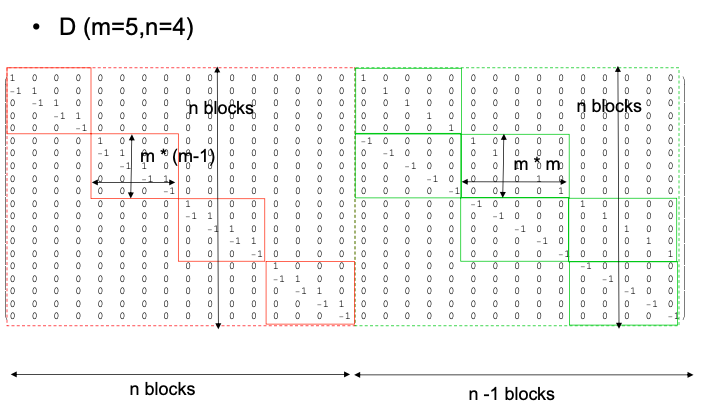
\includegraphics[width=0.75\paperwidth]{D-matrix}
%  }
%  \caption{Divergence matrix.}\label{fig:divergence-matrix}
%\end{figure}

%%%%%%%%%%%%%%%%%%%%%%%%%%%%%%%%%%%%%%%%%%%%%%
% MIGHT WANT TO INCLUDE DERIVATION OF NON-UNIFORM DP/DX 
%% MIGHT ALSO NEED TO CHECK WITH THE PREMULTIPLICATION OF DELTA X
\subsubsection{Gradient}\label{subsec:gradient} 

The pressure gradients are computed at the same coordinates as the unknown velocities according to \cref{eqn:nse-matrix}. Below we will arrive to the conclusion that the discrete gradient and divergence operators satisfy
\begin{equation}\label{eqn:g-dt}
  {G}=-{D^T}
\end{equation}
on staggered/MAC grids. 

\begin{figure}[H] % here, bottom, top
  \centering{
  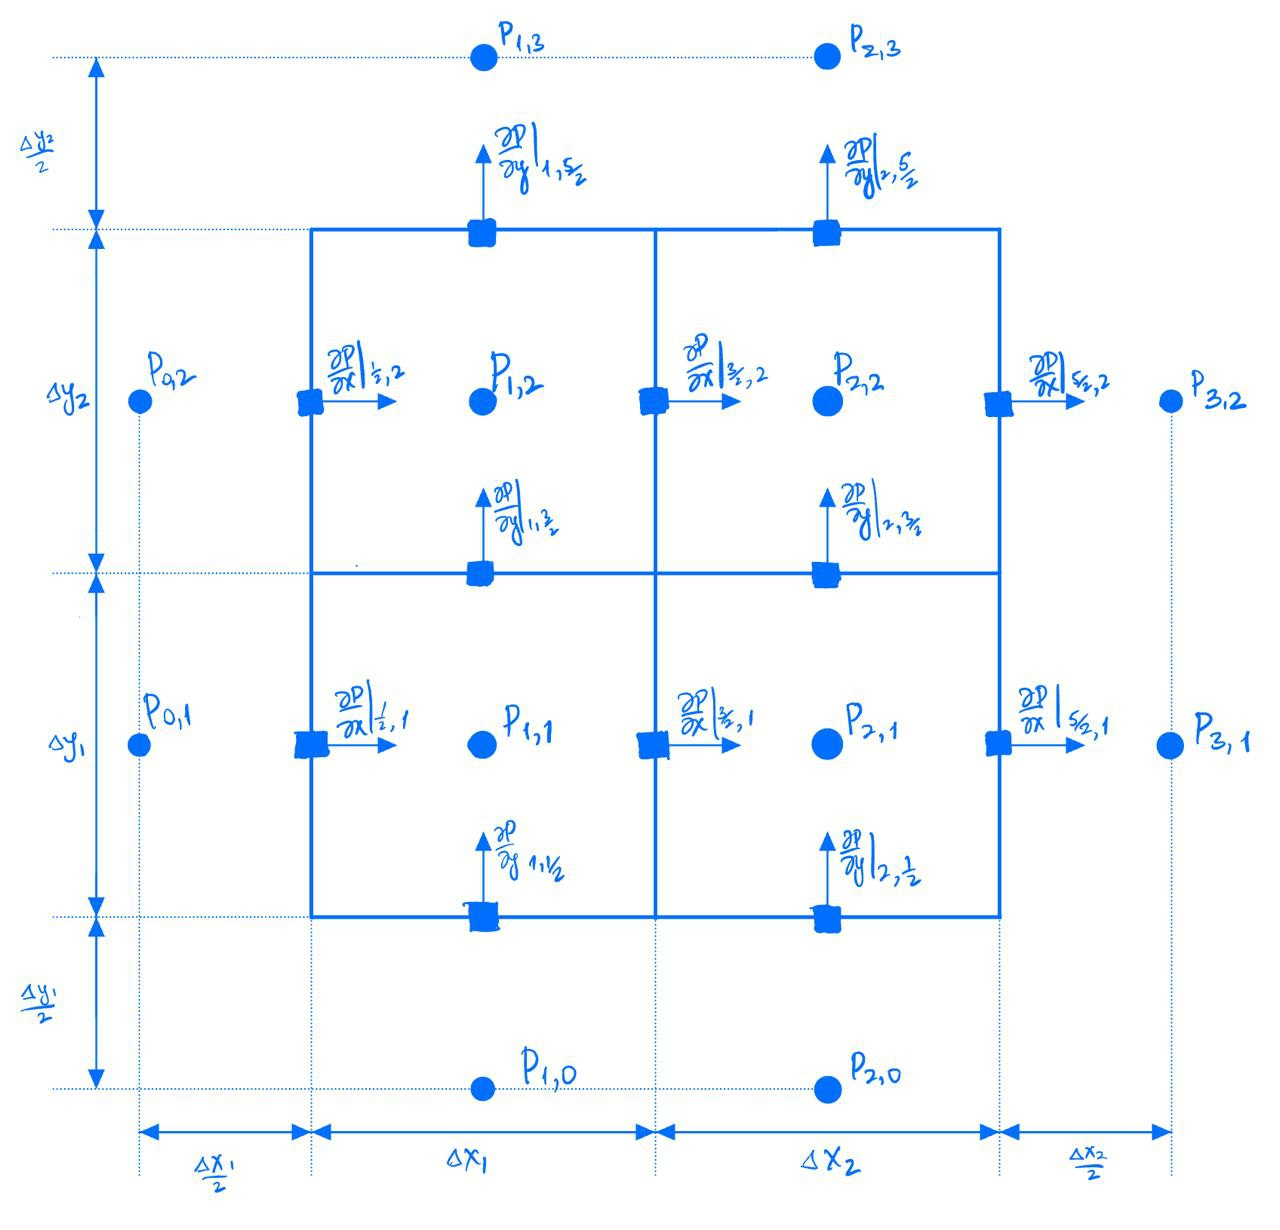
\includegraphics[width=0.65\paperwidth]{G-example-2x2}
  }
  \caption{$2\times 2$ grid example for gradient operator.}\label{fig:G-example-2x2}
\end{figure}


As an illustrative example, we may consider a $2\times 2$ grid as in \cref{fig:G-example-2x2} with the same boundary conditions as in \cref{eqs:NSE-dsm-bl}. It is required to determine the pressure gradients across each unknown velocity (square nodes on \cref{fig:G-example-2x2}):

\begin{alignat*}{2}
	\left.\frac{\partial P}{\partial x}\right|_{\frac{3}{2},1} &=&	\frac{2}{{\Delta x_1 + \Delta x_2}}&\left(P_{1,2}-P_{1,1}\right),\\
	\left.\frac{\partial P}{\partial x}\right|_{\frac{3}{2},2} &=&	\frac{2}{{\Delta x_1 + \Delta x_2}}&\left( P_{2,2}-P_{2,1} \right),\\
	\left.\frac{\partial P}{\partial y}\right|_{1,\frac{3}{2}} &=&	\frac{2}{{\Delta y_1 + \Delta y_2}}&\left(P_{2,1}-P_{1,1} \right),\\
	\left.\frac{\partial P}{\partial y}\right|_{2,\frac{3}{2}} &=&	\frac{2}{{\Delta y_1 + \Delta y_2}}&\left( P_{2,2}-P_{1,2} \right).
\end{alignat*}

The next step is to rewrite the above expressions in matrix form using the pressure boundary conditions outside the grid. The resultant system of linear equations then becomes
\begin{equation}\label[system]{eqn:gradient-matrix}
	\begin{bmatrix}{}
		\frac{2}{\Delta x_1 + \Delta x_2}	&0	&0	&0	\\
		0	&\frac{2}{\Delta x_1 + \Delta x_2}	&0	&0	\\
		0	&0	&\frac{2}{\Delta y_1 + \Delta y_2}	&0	\\
		0	&0	&0	&\frac{2}{\Delta y_1 + \Delta y_2}\\
	\end{bmatrix}
	\begin{bmatrix*}[r]
	-1 & 1 & 0 & 0 \\
	0 & 0 & -1 & 1 \\
	-1 & 0 & 1 & 0 \\
	0 & -1 & 0 & 1
	\end{bmatrix*}
	\begin{bmatrix}{}
  		P_{1,1} \\
	  	P_{2,1} \\
		P_{1,2} \\
		P_{2,2}
	\end{bmatrix}
	=
	\begin{bmatrix}{}
		0\\
		0\\
		0\\
		0
	\end{bmatrix},
\end{equation}
which can be rewritten as
\begin{equation}
	\hat{M}^{-1}{G} 
	\begin{bmatrix}{}
  		p_{1,1} \\
	  	p_{1,2} \\
	  	\vdots \\
	  	p_{MN}
	\end{bmatrix}
=\hat{bc}_p,
\end{equation}
where $\hat{M}^{-1}$ is the diagonal matrix containing the distances between neighbouring pressure coordinates, ${G}$ is the gradient matrix and $[p_1,p_2,...p_{MN}]^T$ is the vector of pressure values at the cell centres. There are no pressure BC values in $\hat{bc}_p$ since no pressure gradient has to be computed across the boundary. It can be observed from \cref{eqn:divergence-matrix,eqn:gradient-matrix} that \cref{eqn:g-dt} holds and the general case is true by construction.

%%%%%%%%%%%%%%%%%%%%%%%%%%%%%%%%%%%%%%%%%%%%%%%%
\subsubsection{Advection}\label{subsec:advection}

%\begin{figure}
%\centering
%{\includegraphics[width=0.75\paperwidth]{advectionGrid.jpg} }
%\caption{\small Advection on a staggered grid.}\label{fig:advectionGrid}
%\end{figure}
Since Explicit Adams-Bashforth~\cref{eqn:nonlinear-adams-bashforth} uses information from time steps $n$ and $n-1$, while we solve the system of equations for time step $n+1$ there is no need for upwinding or even more complicated schemes. For spatial discretization we will try to stick to the central schemes as they are more stable and less dependent on the flow direction. It is convenient to write such schemes for conservative form of the advection, moreover, this also keeps the error low, since there is no product of velocity with acceleration. Hence, let us rewrite advective derivatives in conservative form. 
\begin{align}\label{eqn:advection-conservative}
	u\frac{\partial u}{\partial x}+v \frac{\partial u}{\partial y}
	&=u\frac{\partial u}{\partial x}+0+v \frac{\partial u}{\partial y}\nonumber\\
	&= u\frac{\partial u}{\partial x}+ u\left(\frac{\partial u}{\partial x} +\frac{\partial v}{\partial y}\right ) +v \frac{\partial u}{\partial y}\nonumber\\
	&=\left(u\frac{\partial u}{\partial x}+ u\frac{\partial u}{\partial x}\right ) +\left(u\frac{\partial v}{\partial y} +v \frac{\partial u}{\partial y}\right )\nonumber\\
	&=\frac{\partial uu}{\partial x}+ \frac{\partial uv}{\partial y}.
\end{align}
Our goal is to compute advection components at the unknown velocity coordinates. Below we will describe the discretization schemes for \cref{eqn:advection-conservative}. 

\textbf{Inner part.} 
Advective component from $x$-momentum was expressed in conservative form by \cref{eqn:advection-conservative}. It is discretized using the standard central differencing schemes~\cite{Colonius:2008} as
\begin{align}\label{eqn:adv-inner}
	\left (u\frac{\partial u}{\partial x}+v \frac{\partial u}{\partial y}\right)_{i-\frac{1}{2},j}&=\frac{(uu)_{i
	,j}-(uu)_{i- 1,j}}{\frac{\Delta x_i+\Delta x_{i-1}}{2}}+\frac{(uv)_{i-\frac{1}{2},j+\frac{1}{2}}-(uv)_{i-\frac{1}{2},j-\frac{1}{2}}}{\Delta y_i},
\end{align}
which is evaluated at the same points as $u_{i-\frac{1}{2},j}$ (squares in \cref{fig:ADV}). We need to compute $uv$ at the nodes and $uu$ at cell centres, which are triangles and circles respectively in \cref{fig:ADV}. Using linear interpolation~\cite{Colonius:2008} of velocity values leads to
\begin{align*}
  (uu)_{i,j}&=\left(\frac{u_{i+\frac{1}{2},j}+u_{i-\frac{1}{2},j}}{2}\right)^2,\\
  (uv)_{i-\frac{1}{2},j-\frac{1}{2}}&=\left(u_{i-\frac{1}{2},j-1} + \frac{\Delta y_{j-1}}{2}\frac{u_{i-\frac{1}{2},j}-u_{i-\frac{1}{2},j-1}}{\frac{\Delta y_{j-1} +\Delta y_j}{2}} \right) \left( v_{i-1,j-\frac{1}{2}} + \frac{\Delta x_{i-1}}{2}\frac{v_{i,j-\frac{1}{2}}-v_{i-1,j-\frac{1}{2}}}{\frac{\Delta x_{i-1} +\Delta x_i}{2}}\right)\\
  &=\left(\frac{u_{i-\frac{1}{2},j}\Delta y_{j-1} +u_{i-\frac{1}{2},j-1}\Delta y_j}{\Delta y_{j-1}+\Delta y_{j}}\right )\left ( \frac{v_{i,j-1\frac{1}{2}}\Delta x_{i-1} +v_{i-1,j-\frac{1}{2}}\Delta x_i}{\Delta x_{i-1}+\Delta x_{i}}\right).
\end{align*}

\begin{figure}[H] % here, bottom, top
  \centering{
  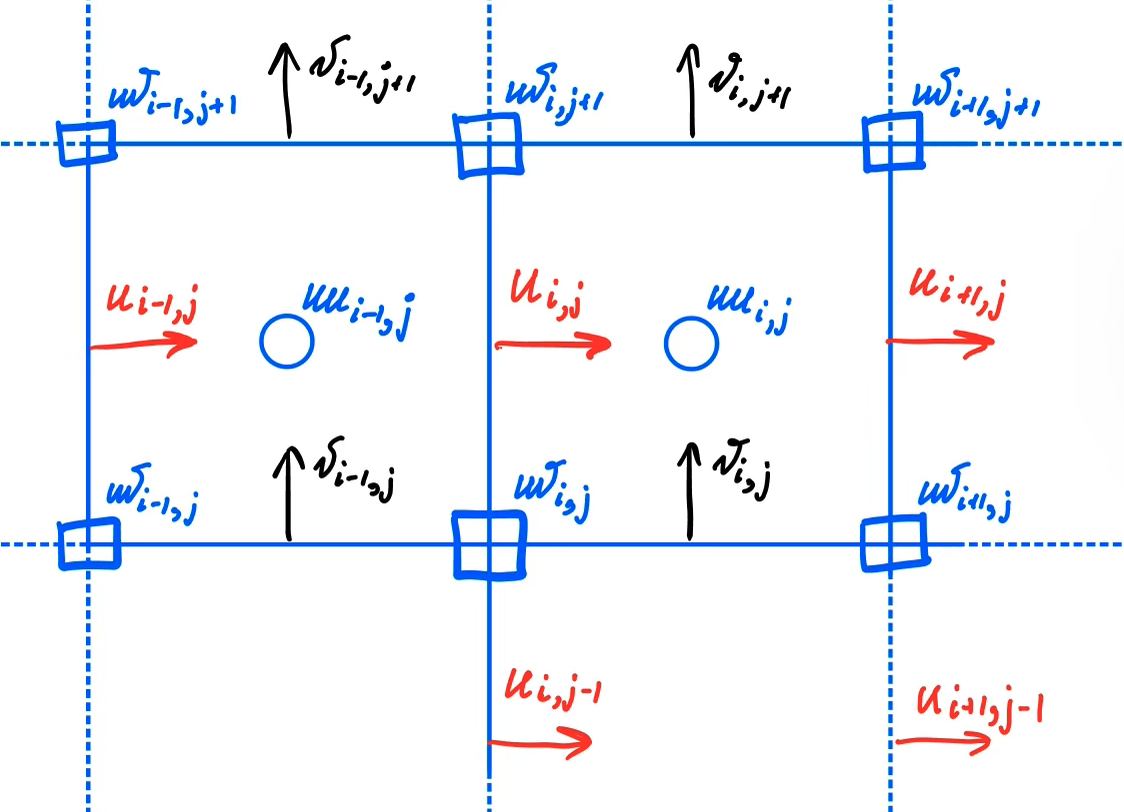
\includegraphics[width=0.65\paperwidth]{ADV}
  }
  \caption{Advection discretization.}\label{fig:ADV}
\end{figure}


\textbf{Right boundary (outlet).}
\begin{figure}[H] % here, bottom, top
  \centering{
  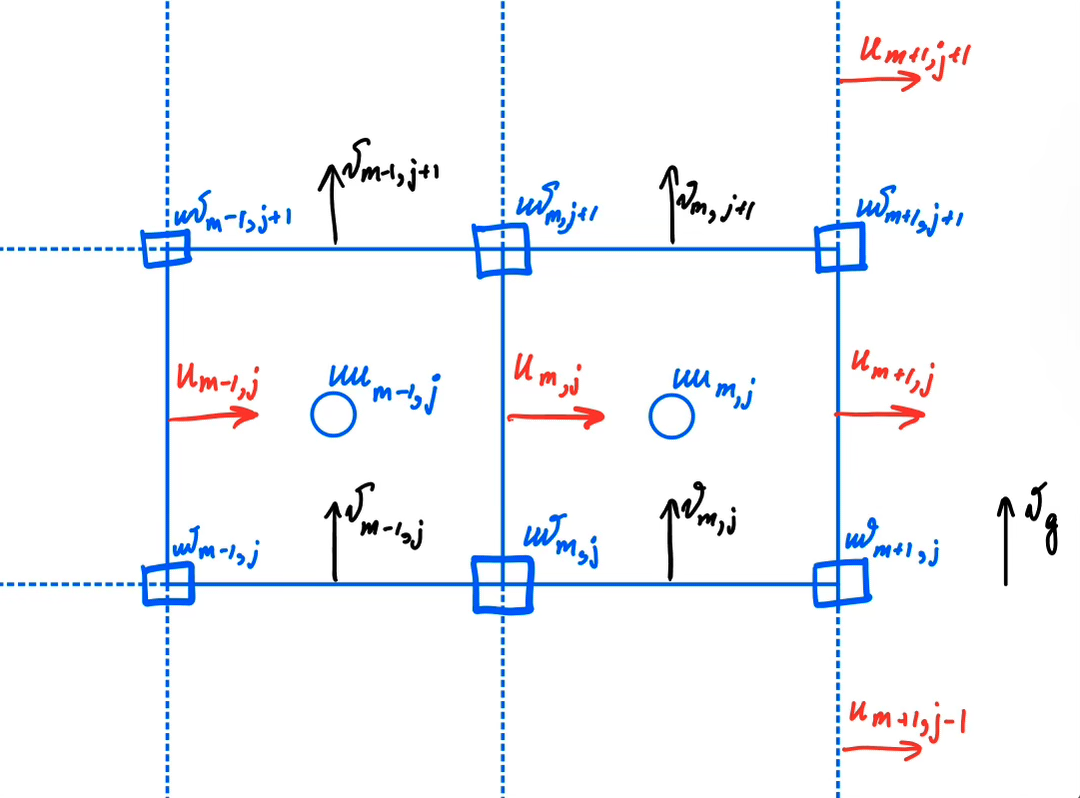
\includegraphics[width=0.45\paperwidth]{ADV-right}
  }
  \caption{Right boundary advection.}\label{fig:ADV-right}
\end{figure}
\cref{eqn:bc-u-right} rewritten for the time step $n$ is
\begin{equation*}
\begin{gathered}
{{u}^{n}_{M+\frac{1}{2},j}}\left(\frac{1}{\Delta t} + \frac{u^{n-1}_{M+\frac{1}{2},j}}{2\Delta x_M}\right)
=
u^{n}_{M-\frac{1}{2},j}\frac{u^{n-1}_{M+\frac{1}{2},j}}{2\Delta x_M}+bc_e^{n-1}.
\end{gathered}
\end{equation*}
This can be used to obtain the value $u^{n}_{M+\frac{1}{2},j}$ at the right boundary. Then we use the \cref{eqn:adv-inner} for inner part as now all the necessary values are known. Similarly, \cref{eqn:bc-v-right} at time step $n$
\begin{equation*}
\begin{gathered}
\left( \frac{1}{2\Delta t} + \frac{u^n_{M+\frac{1}{2},j-\frac{1}{2}}}{2\Delta x_{M+\frac{1}{2}}}\right) v^{n}_{M+1,j-\frac{1}{2}}
=\left( -\frac{1}{2\Delta t}+\frac{u^n_{M+\frac{1}{2},j-\frac{1}{2}}}{2\Delta x_{M+\frac{1}{2}}} \right)v^{n}_{M,j-\frac{1}{2}}+bc_{ve}^{n-1}
\end{gathered}
\end{equation*}
is used to express ghost velocity $v^{n}_{M+1,j-\frac{1}{2}}$, which we use to compute \cref{eqn:adv-inner} for inner part.


%One of the advantages of advective boundary condition $\frac{\partial u}{\partial t}+u\frac{\partial u}{\partial x}=0$ (or  $\frac{\partial u}{\partial t}+u\frac{\partial u}{\partial x}=\nu \frac{\partial^2 u}{\partial y^2}$) is that it can be used to express $\frac{\partial uu}{\partial x}$ in terms of transient term as 
%\begin{equation}
%	\left( \frac{\partial uu}{\partial x}\right)_{m+\frac{1}{2},j}=2\left( u \frac{\partial u}{\partial x}\right)_{m+\frac{1}{2},j}=2\left( -\frac{\partial u}{\partial t}\right)_{m+\frac{1}{2},j},
%\end{equation}
%or in terms of transient and diffusive components
%\begin{equation}
%	\left( \frac{\partial uu}{\partial x}\right)_{m+\frac{1}{2},j}=2\left( u \frac{\partial u}{\partial x}\right)_{m+\frac{1}{2},j}=2\left( -\frac{\partial u}{\partial t}+\nu\frac{\partial ^2 u}{\partial y^2}\right)_{m+\frac{1}{2},j}.
%\end{equation}
%
%The other advection summand
%\begin{equation}
%	\left(\frac{\partial uv}{\partial y}\right)_{m+\frac{1}{2},j}=\frac{\left( uv \right)_{m+\frac{1}{2},j+\frac{1}{2}}-\left( uv\right)_{m+\frac{1}{2},j-\frac{1}{2}}}{\Delta}
%\end{equation}
%requires values of $v$ at the nodes $m+\frac{1}{2},j\pm \frac{1}{2}$. We may use two neighbouring $v$ components and extrapolate them linearly as 
%\begin{equation}
%	v_{m+\frac{1}{2},j+\frac{1}{2}}=v_{m-1,j\pm\frac{1}{2}}+2\frac{v_{m,j\pm\frac{1}{2}}-v_{m-1,j\pm\frac{1}{2}}}{\Delta x_{m-1}+\Delta x_m}\left(\Delta x_m + \frac{1}{2}\Delta x_{m-1}\right).
%\end{equation}

\textbf{Left boundary (inlet).} 
\begin{figure}[H] % here, bottom, top
  \centering{
  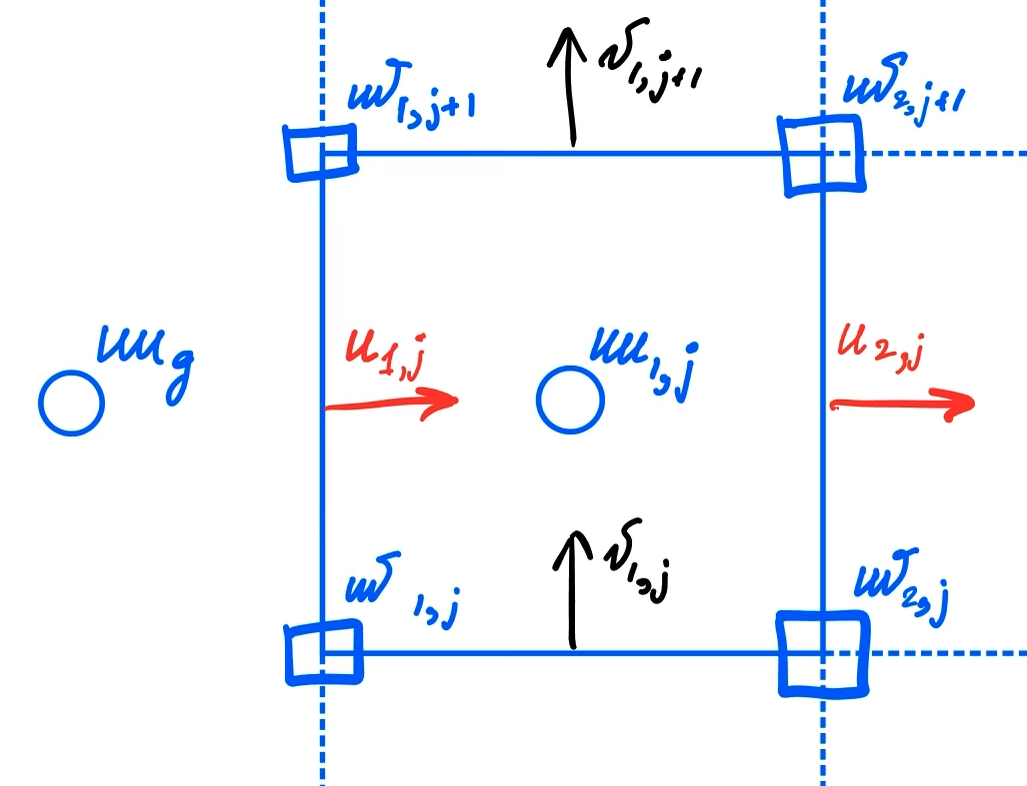
\includegraphics[width=0.30\paperwidth]{ADV-left}
  }
  \caption{Left boundary advection.}\label{fig:ADV-left}
\end{figure}
The exact value of the $uu_g$ element located outside the boundary (\cref{fig:ADV-left}) is known from the inlet boundary conditions, whereas $uv_{\frac{1}{2},j}$ is zero for all $j$ due to $v_{bc}=0$ at the inlet. 

\textbf{Top boundary (symmetric).}
\begin{figure}[H] % here, bottom, top
  \centering{
  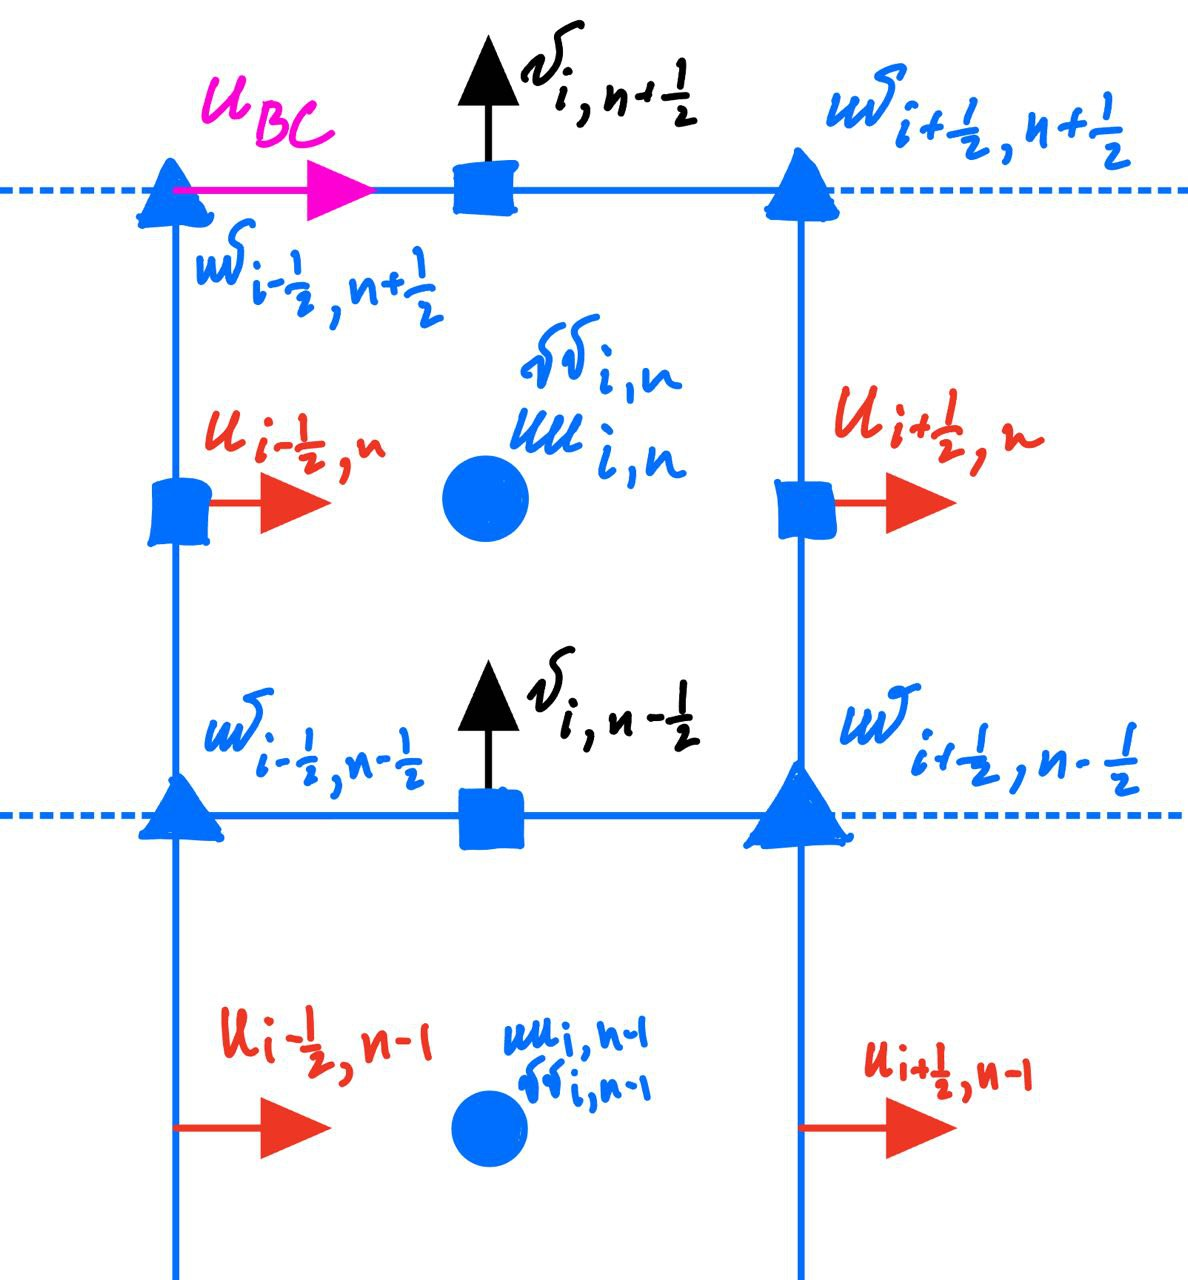
\includegraphics[width=0.35\paperwidth]{ADV-top}
  }
  \caption{Top boundary advection.}\label{fig:ADV-top}
\end{figure}
%The symmetric \cref{eqn:symmetric-bc} defines a mirror surface, which has the same effect on the solution as the semi-infinite boundary condition if the boundary layer thickness is less than the truncated domain height. Mathematically such boundary condition can be written as $v=\frac{\partial v}{\partial y}=0,\frac{\partial p}{\partial y}=0$. 
Since the exact values of the velocity $u_{BC}$ and $v_{BC}=0$ in a freestream are known from \cref{eqn:symmetric-bc}, we can directly use them in our advection term computation making the second summand $uv=0$, in particular
\begin{equation}
	\left( \frac{\partial uu}{\partial x}+\frac{\partial uv}{\partial y}\right)_{i-\frac{1}{2},N}=2\frac{\left( uu\right)_{i,N}-\left( uu\right)_{i-1,N}}{\Delta x_i + \Delta x_{i-1}}+0.
\end{equation}

\textbf{Bottom boundary (no-slip).}
\begin{figure}[H] % here, bottom, top
  \centering{
  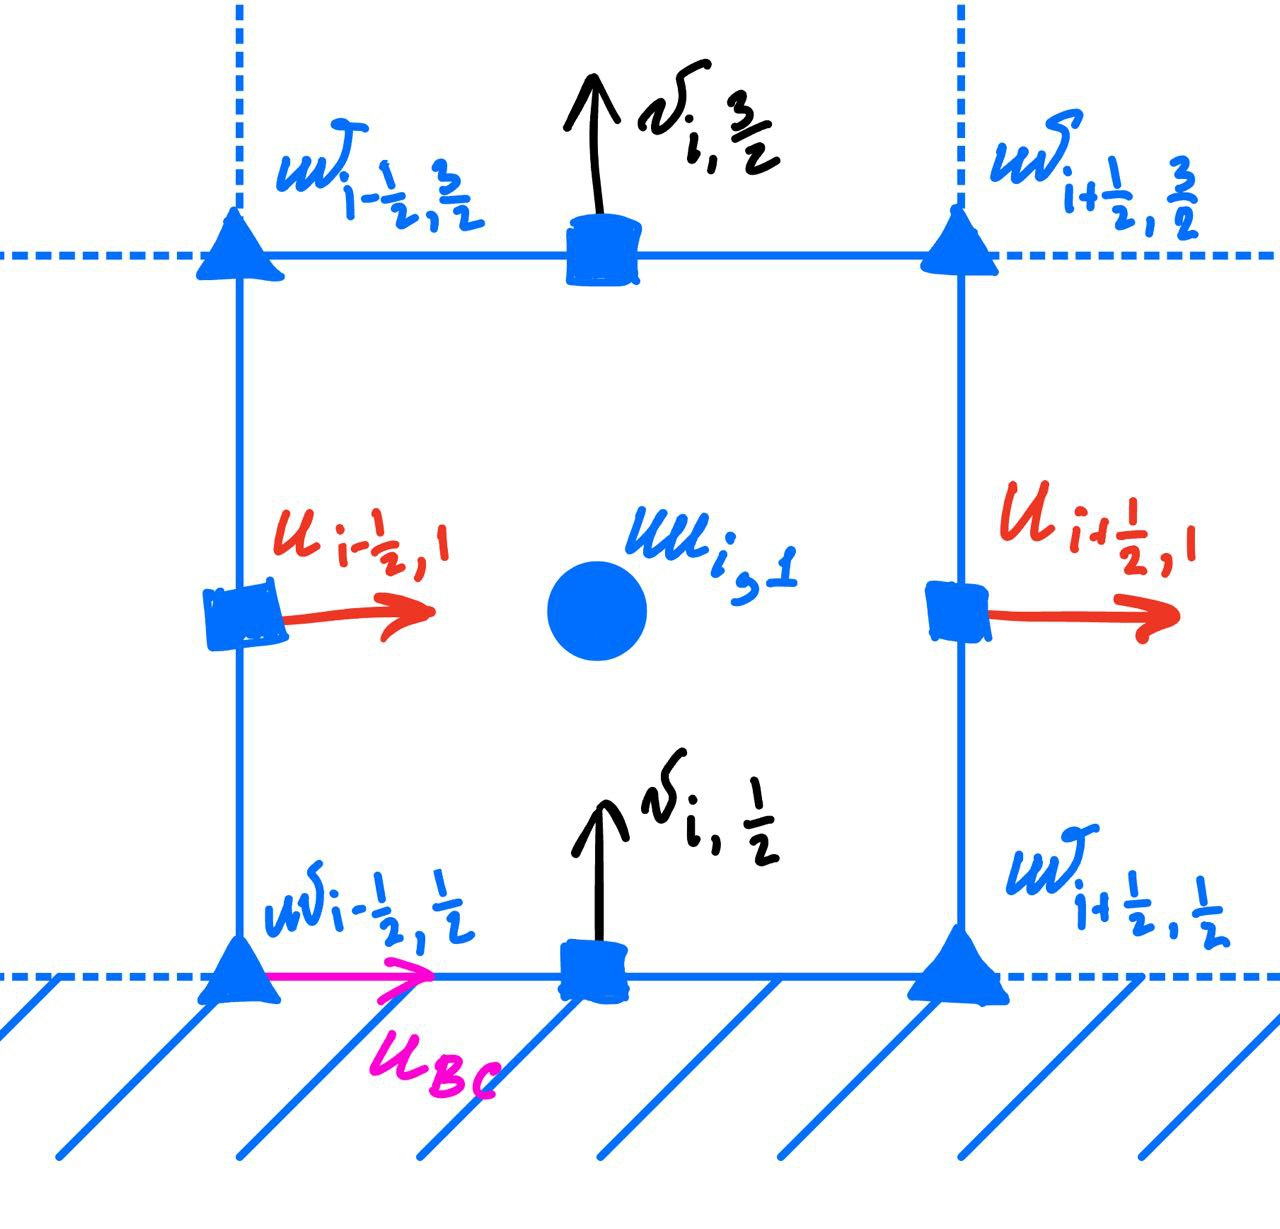
\includegraphics[width=0.30\paperwidth]{ADV-bottom}
  }
  \caption{Bottom boundary advection}\label{fig:ADV-bottom}
\end{figure}
Computation of the advective terms just above the bottom boundary is the same as for the inner part, with the only exception being $uv_{i-\frac{1}{2},\frac{1}{2}}=0$ at the boundary, due to the $u_{bc}=0$ condition on the plate (purple on \cref{fig:ADV-bottom}).

The advective terms in the $y$-momentum equation are computed similarly. After the derivatives are evaluated, they are moved to the right-hand side as in \cref{eqn:NSE-dsm-bl-system-schemes} and treated explicitly. 

%\subsubsection{Resulting system}



%%%%%%%%%%%%%%%%%%%%%%%%%%%%%%%%%%%%%%%%%%%%%%%%
%%%%%%%%%%%%%%%%%%%%%%%%%%%%%%%%%%%%%%%%%%%%%%%%
%%%%%%
%%%%%%		TYPOS CHECK FROM BELOW  %%%%%%%%%%%%
%%%%%%
%%%%%%%%%%%%%%%%%%%%%%%%%%%%%%%%%%%%%%%%%%%%%%%%
%%%%%%%%%%%%%%%%%%%%%%%%%%%%%%%%%%%%%%%%%%%%%%%%
%Overall, we have $N_x, N_y$ nodes in the $x$ and $y$ direction respectively. 
%There are $N_u=(N_x-1)N_y+N_y$ elements of $u$, where extra $N_y$ is added to account for the unknown outlet boundary velocities. $N_v=N_x(N_y-1)$ represents the number of velocity components within vector $v$. Define $N_{tot}=N_u+N_v$.
%               
%Then the matrices in equation~\eqref{eqn:nse-matrix} have dimensions of:
%\begin{itemize}
%	\item[$\mathbf{I}$] - [$N_{tot}\times N_{tot}$];
%	\item[$\hat{D}$] - [$(N_xN_y)\times(N_{tot})$];
%	\item[$\hat{G}$] - [$(N_{tot})\times(N_xN_y)$];
%	\item[$\mathbf{\hat{H}}$] - [$N_{tot}\times 1$];
%	\item[$\hat{L}$] - [$N_{tot}\times N_{tot}$];
%	\item[bc] - [$N_{tot}\times 1$], which are inhomogeneous terms from the Boundary Conditions vector.
%\end{itemize}        
%
%Attack the system~\eqref{eqn:nse-matrix} with the following (listed in the appendix) schemes:
%\begin{enumerate}
%	\item[\textbf{Viscous}]: Implicit trapezoidal - Crank Nicholson~\eqref{eqn:crank-nicholson} scheme.  
%  \item[\textbf{Nonlinear (advect.)}]: Explicit Adams-Bashforth~\eqref{eqn:adams-bashforth} as in Figure~\ref{fig:Advection-discretization}. 
%	\item[\textbf{Pressure}]: Implicit Euler~\eqref{eqn:implicit-euler}, however the pressure variable is not used in computations. 
%\end{enumerate}
%
%The above discretization schemes result in the following discretized system:
%\begin{equation*}
%	\begin{bmatrix}
%		\frac{1}{\Delta t}\mathbf{I}-\frac{1}{2}\hat{L} & \hat{G} \\
%		\hat{D} & 0
%	\end{bmatrix}
%	\begin{pmatrix}
%		\boldsymbol{v}^{n+1} \\ 
%		p
%	\end{pmatrix}
%	=
%	\begin{pmatrix}
%		\left[\frac{1}{\Delta t}\mathbf{I}-\frac{1}{2}\hat{L}\right]u^n - \left[\frac{3}{2}\hat{N}(\boldsymbol{v}^n) - \frac{1}{2}\hat{N}(\boldsymbol{v}^{n-1})\right]\\
%		0
%	\end{pmatrix}
%	+
%	\begin{pmatrix}
%		\hat{bc}_1\\
%		\hat{bc}_2
%	\end{pmatrix}.
%\end{equation*}
%
%After introduction of new variables $\hat{A}$ and $\hat{r}^n$ the above system can be rewritten as
%\begin{equation}
%	\begin{bmatrix}
%		\hat{A} & \hat{G} \\
%		\hat{D} & 0
%	\end{bmatrix}
%	\begin{pmatrix}
%		\boldsymbol{v}^{n+1} \\ 
%		p
%	\end{pmatrix}
%	=
%	\begin{pmatrix}
%		\hat{r}^n \\
%		0
%	\end{pmatrix}
%	+
%	\begin{pmatrix}
%		\hat{bc}_1\\
%		\hat{bc}_2
%	\end{pmatrix}.
%\end{equation}
%
%
%\begin{figure}
%\begin{center}
%  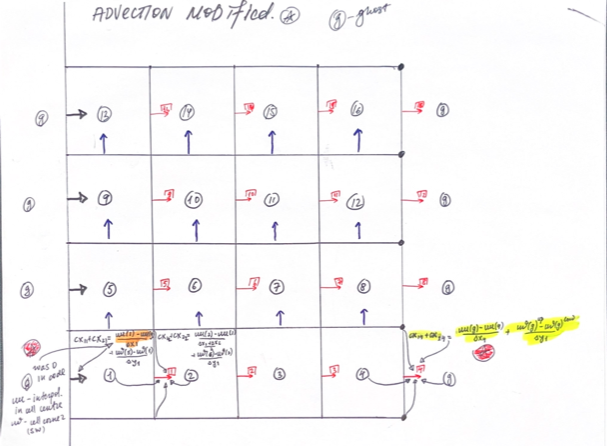
\includegraphics[width=0.75\textwidth]{Figures/advectionGridNew}
%\end{center}
%\caption{Advection discretization.}
%\label{fig:Advection-discretization}
%\end{figure}
%


\subsection{Symmetrization}\label{subsec:symmetrization}

The most effective methods for solving systems of linear equations often work optimally with symmetric matrices, making symmetry a desirable property. In order to achieve a symmetric system, we introduce two matrices - the diagonal scaling matrix $\hat{M}$ and the diagonal flux matrix $R$. These matrices are defined as
\begin{align*}
R &\equiv\left[\begin{array}{cc}
\Delta y_j & 0 \\
0 & \Delta x_i
\end{array}\right], \\
\quad \hat{M} & \equiv\left[\begin{array}{cc}
\frac{1}{2}\left(\Delta x_i+\Delta x_{i-1}\right) & 0 \\
0 & \frac{1}{2}\left(\Delta y_j+\Delta y_{j-1}\right)
\end{array}\right].
\end{align*}
 % and $\hat{D}R^{-1}=-(\hat{M}\hat{G})^T$. I THINK THIS WRONG BUT WRITTEN IN TAIRA DISSERTATION ON PAGE 101.

%The only matrix which can be asymmetric in~\cref{eqn:NSE-dsm-bl-system-schemes} is a Laplacian if the grid is non-uniform. In order to get a symmetric diffusion matrix we need to move to the new variables. 
Define matrices 
\begin{equation*}
\begin{aligned}
	\Delta y_j&=\text{diag}([\underbrace{\Delta y_1; \Delta y_1; \dotsc;\Delta y_1}_{M-1\text{ times}}; \underbrace{\Delta y_2; \Delta y_2; \dotsc;\Delta y_2}_{M-1\text{ times}};\dotsc;\underbrace{\Delta y_N; \Delta y_N; \dotsc;\Delta y_N}_{M-1\text{ times}}]),\\
	\Delta x_i&=\text{diag}([\underbrace{\Delta x_1; \Delta x_2;\dotsc\Delta x_M;\Delta x_1; \Delta x_2;\dotsc\Delta x_M; \dotsc;\Delta x_1; \Delta x_2;\dotsc;\Delta x_M}_{N-1\text{ blocks of } 1,\dotsc,M}]),
\end{aligned}
\end{equation*}
which are then combined into
\begin{equation*}
R =\left[\begin{array}{cc}
\Delta y_j & 0 \\
0 & \Delta x_i
\end{array}\right].
\end{equation*}

Let the new vector variable (mass flux) of unknowns be defined as
$${q} = R\boldsymbol{v},$$ 
where $R$ is a diagonal matrix of size $(M-1)N\times M(N-1)$. Using the $R$ matrix we can express mass flux $q^{n+1}=R\boldsymbol{v}^{n+1}\implies \boldsymbol{v}^{n+1}=R^{-1}q^{n+1}$. It is required that the difference matrices cancel out $\frac{x_{i+1}-x_{i-1}}{2}$ central term in diffusion discretization to make Laplacian symmetric. Define the elements of diagonal mass matrix as
\begin{equation*}
{\Delta x_i+\Delta x_{i-1}} = \text{diag}[\underbrace{\Delta x_2+\Delta x_1; \Delta x_3+\Delta x_2; \dotsc ;\Delta x_{M}+\Delta x_{M-1}; ...;\Delta x_2+\Delta x_1; \Delta x_3+\Delta x_2; \dotsc \Delta x_{M}+\Delta x_{M}}_{N\text{ times for each block of } \Delta x_2+\Delta x_1\text{ to }\Delta x_{M}+\Delta x_{M-1}}]
\end{equation*}
and
\begin{equation*}
{\Delta y_j+\Delta y_{j-1}} = \text{diag}[\underbrace{\Delta y_2+\Delta y_1;  \dotsc \Delta y_2+\Delta y_1;}_{M\text{ times}} \underbrace{\Delta y_3+\Delta y_2; \dotsc \Delta y_3+\Delta y_2;}_{M\text{ times}} \underbrace{\Delta y_N+\Delta y_{N-1}\dotsc \Delta y_N+\Delta y_{N-1}}_{M\text{ times}}],	
\end{equation*}
which are then combined into
\begin{equation*}
\hat{M} =\left[\begin{array}{cc}
\frac{1}{2}\left(\Delta x_i+\Delta x_{i-1}\right) & 0 \\
0 & \frac{1}{2}\left(\Delta y_j+\Delta y_{j-1}\right)
\end{array}\right].
\end{equation*}

The identity ${q}=R\boldsymbol{v}$ implies $\boldsymbol{v}=R^{-1}{q}$, therefore, Laplacian matrix multiplied by the velocity vector is
$$L\boldsymbol{v}= LR^{-1}{q},$$ 
premultiplying by $\hat M$ we obtain
$$\hat MLR^{-1}{q},$$ 
where $\hat M L R^{-1}$ is symmetric by construction.  

Using the above transformations we can modify \cref{eqn:NSE-dsm-bl-system-nonint}
%\begin{equation*}
%\left[\begin{array}{ccc}
%\hat{A} & \hat{G} \\
%\hat{D} & 0 
%\end{array}\right]\left(\begin{array}{c}
%\boldsymbol{v}^{n+1} \\
%p
%\end{array}\right)=\left(\begin{array}{c}
%\hat{r}^n \\
%0 
%\end{array}\right)+\left(\begin{array}{c}
%\widehat{bc}_1 \\
%\widehat{bc}_2 
%\end{array}\right)
%\end{equation*}
into 
\begin{equation*}
\left[\begin{array}{cc}
\hat{M}\hat{A}R^{-1} & \hat{M}\hat{G} \\
\hat{D}R^{-1} & 0
\end{array}\right]\left(\begin{array}{c}
q^{n+1} \\
p^{n+1}
\end{array}\right)=\left(\begin{array}{c}
\hat{M}\hat{r}^n \\
0
\end{array}\right)+\left(\begin{array}{c}
\hat{M}\widehat{b c}_1 \\
\widehat{b c}_2
\end{array}\right),
\end{equation*}
which can be rewritten as 
\begin{equation}\label[system]{eqn:nse-normalized}
\left[\begin{array}{cc}
A & G \\
D & 0
\end{array}\right]\left(\begin{array}{c}
q^{n+1} \\
p^{n+1}
\end{array}\right)=\left(\begin{array}{c}
r^n \\
0
\end{array}\right)+\left(\begin{array}{c}
{b c}_1 \\
{b c}_2
\end{array}\right),
\end{equation}
where $A=\hat{M}\hat{A}R^{-1}=\frac{1}{\Delta t}\hat{M}R^{-1}-\frac{1}{2}\hat{M}\hat{L}R^{-1}$ is symmetric and $\hat{G}=\hat{M}^{-1}G$ according to \cref{eqn:gradient-matrix}. It is also possible to transform the divergence operator $\hat{D}$ with non-integer coefficients into $D$ with integer coefficients in continuity part of \cref{eqn:nse-normalized} using  \cref{eqn:divergence-matrix}. Multiplying both sides of continuity equation by $\Delta _{xy}$ matrix from \cref{eqn:delta-xy} leads to 
\begin{align*}
	\hat{D}\boldsymbol{v}^{n+1}&= \hat{bc}_2\notag\\
	\left(\Delta_{xy} \right)\hat{D}\boldsymbol{v}^{n+1}&=\left ( \Delta_{xy}\right ) \hat{bc}_2\notag\\
	\left(\Delta_{xy}\right)\frac{1}{\Delta _{xy}}{D}R\boldsymbol{v}^{n+1}&=\left ( \Delta_{xy}\right ) \hat{bc}_2\notag\\
	\left(\Delta_{xy}\right)\frac{1}{\Delta_{xy}}{D}q^{n+1}&=\left ( \Delta_{xy}\right ) \hat{bc}_2\notag\\
	D{q}^{n+1}&=bc_2.
\end{align*}

\subsection{Nullspace method and pressure elimination}\label{sec:nullspace-method}

The goal of this subsection is to show how unknown pressure variables can be eliminated from \cref{eqn:nse-normalized}. Publications of Chang~\cite{Chang:2002} and Hall~\cite{Hall:1980} use the idea that in \cref{eqn:nse-normalized} matrix $D$ is wider than tall for grids larger than $2\times 2$, hence it defines a nullspace. The nullspace of matrix $D$ is the set of all solutions to the homogeneous linear system $Dx = 0$, where $x$ is a vector in the null space of $D$. Let $C$ be the nullspace matrix containing such vectors $x$. 

The number of rows in the nullspace $C$ is equal to the number of faces with unknown velocities ($N_f$). In two dimensions $C$ has $N_n$ columns, which is equal to the number of nodes in the grid, whereas in three dimensions the nullspace has $N_e$ columns being the number of edges. 

In the two-dimensional case, the matrix $C$ has two non-zero elements in each row, which are $+1$ and $-1$. The $+1$ value corresponds to the node $90^\circ$ from the normal velocity vector, whereas $-1$ corresponds to the node $-90^\circ$ from the normal velocity vector.  For three dimensional case see Chang ~\cite{Chang:2002}.

%A more intuitive way of constructing the matrix $C$ relies on the usage of a counterclockwise vorticity around the nodes inside the domain and the boundary if such nodes have adjacent velocities from $\boldsymbol{v}$. In the case of the open boundary vortices around the nodes belonging to the open segment are taken into consideration. If the direction of the velocity vector on the adjacent face matches the direction of the vorticity then $+1$ is put into the corresponding row, $-1$ in case of the opposite directions of the velocity and vorticity. The matrix $C$ has the dimension of unknown velocities times the number of nodes around which these velocities revolve. Figure~\ref{fig:DC} shows matrices $D$ and $C$ for a $4\times4$ grid case with an open boundary on the right side of the domain. Yellow squares indicate $+1$, whereas blue squares correspond to $-1$ entries. The desired product then becomes $DC=0$ and since $D=-G^T$ we also have $(DC)^T=C^TD^T=-C^TG=0$. 

A more intuitive way of constructing the matrix $C$ relies on the utilization of counterclockwise vorticity around the nodes within the domain (\cref{fig:C-example-2x2}). If the direction of the velocity vector on the adjacent face aligns with the vorticity's direction, +1 is assigned to the corresponding row; conversely, -1 is assigned in the case of opposite directions of velocity and vorticity. After applying the above procedure we obtain
\begin{equation*}
  C = 
  \begin{bmatrix*}[r]
  1		\\
%  0		\\
  -1	\\
%  0		\\
  -1	\\
  1		\\
\end{bmatrix*}.
\end{equation*}

\begin{figure}[h] % here, bottom, top
  \centering{
  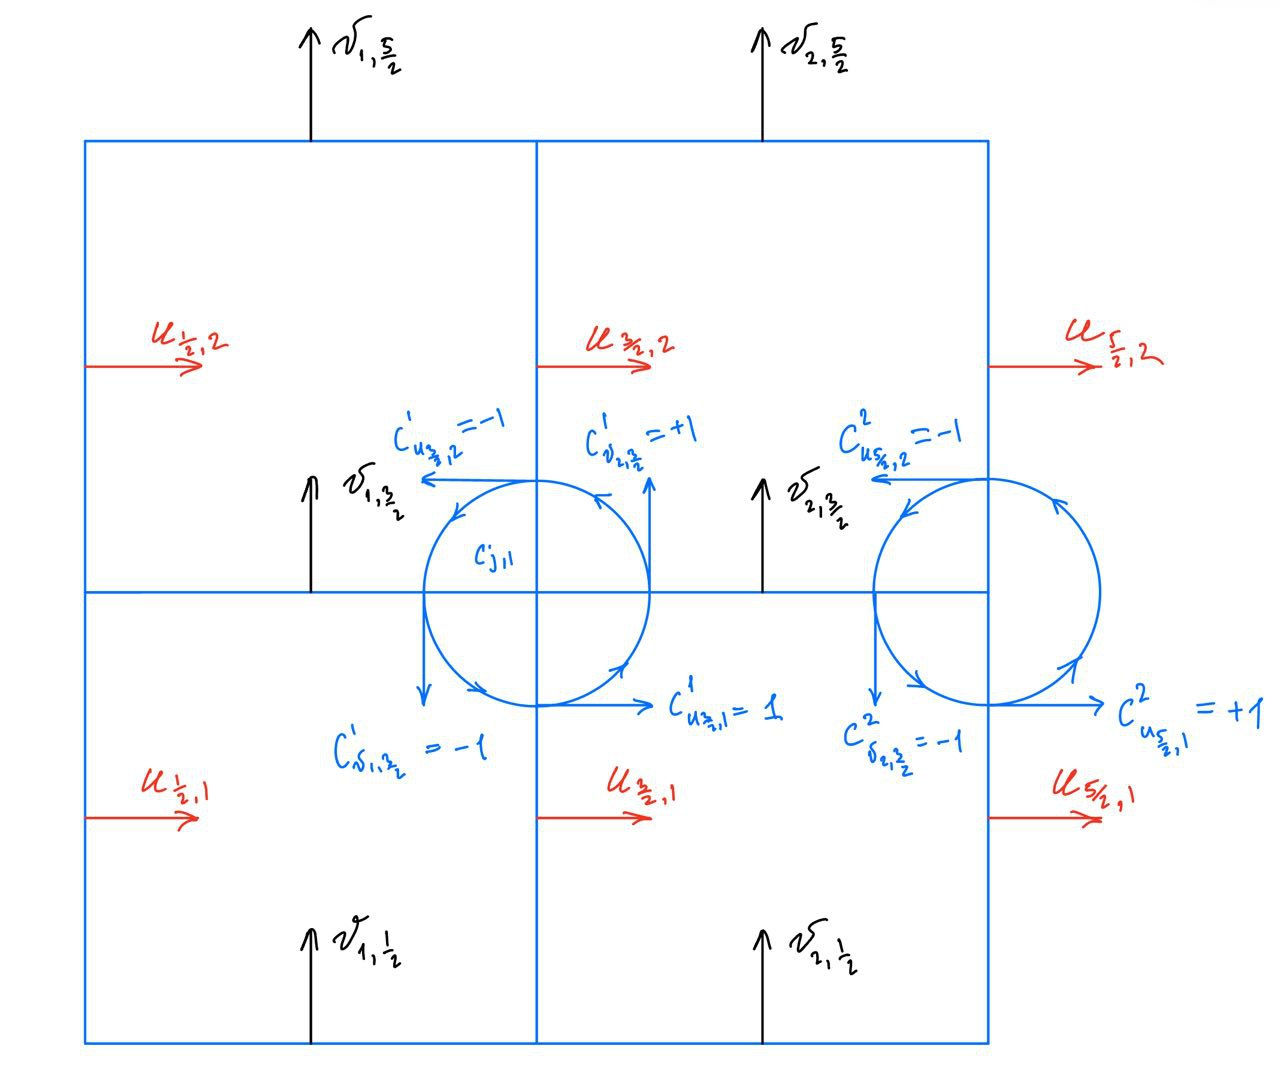
\includegraphics[width=0.45\paperwidth]{C-example-2x2}
  }
  \caption{$2\times 2$ example for $C$ matrix.}\label{fig:C-example-2x2}
\end{figure}


The matrix $C$ has dimensions corresponding to unknown velocities times the number of nodes around which these velocities revolve. Figure~\ref{fig:DC} illustrates matrices $D$ and $C$ for a $4\times4$ grid with an open boundary on the right side of the domain. 
%Yellow squares represent $+1$ entries, while blue squares correspond to $-1$. 

The desired product then becomes $DC=0$. $D=-G^T$ (\cref{subsec:divergence,subsec:gradient}) leads to important property $(DC)^T=C^TD^T=-C^TG=0$. Premultiplying momentum equation in \cref{eqn:nse-normalized} by $C^T$ creates $C^TGp=0$ term, which completely eliminates the pressure from our system.

In order to make use of efficient solvers, the system $C^TA$ can be made symmetric if multiplied by $C$ from the right. Hence, the final chord of this method is the introduction of another new variable called discrete streamfunction $\psi:q_h=C\psi$, where $q_h$ is a homogeneous solution to the \cref{eqn:nse-normalized} from \cref{subsec:symmetrization} and is discussed in the following \cref{sec:algorithm}.

\begin{figure}
\begin{center}
  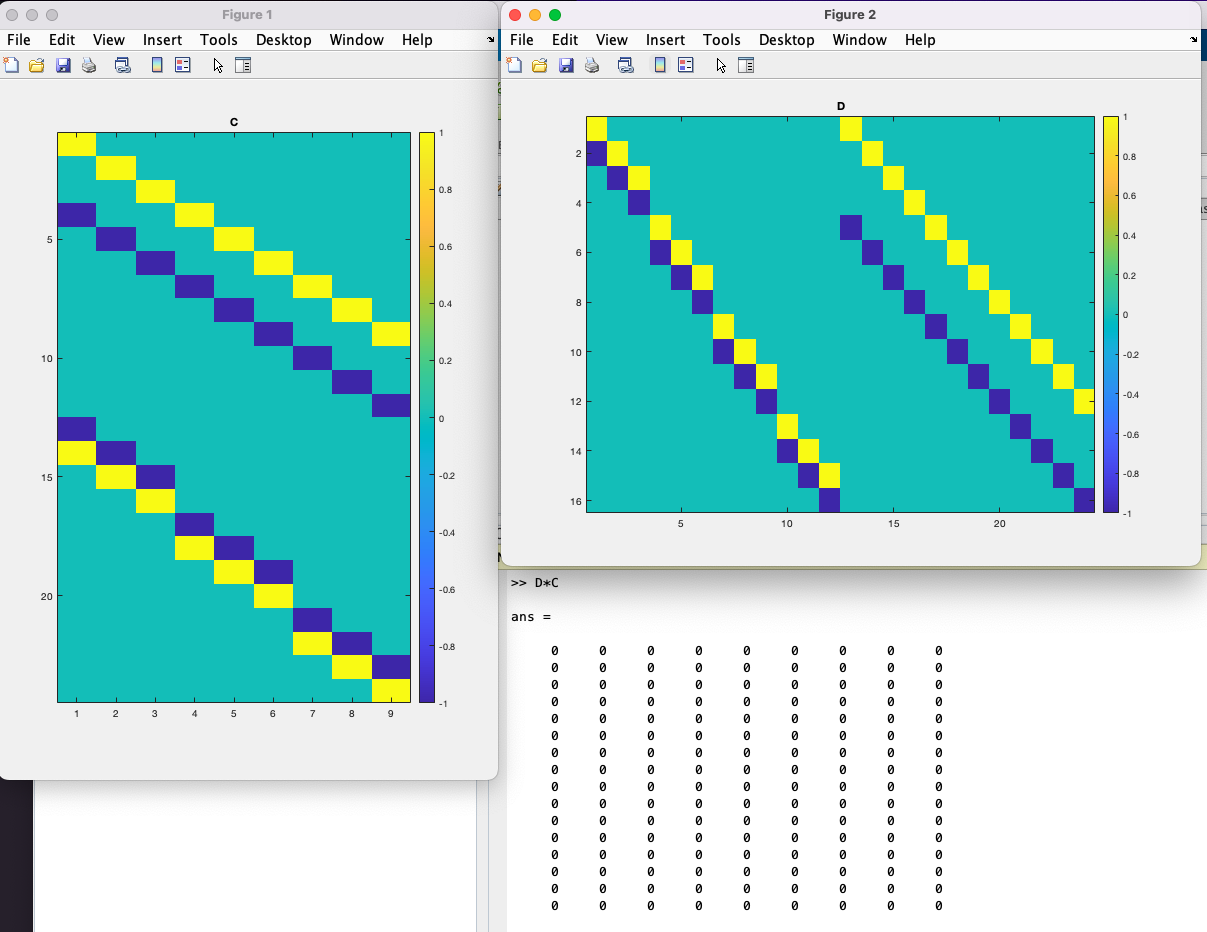
\includegraphics[width=0.75\textwidth]{Figures/D-C-DC}
\end{center}
\caption{Divergence and Curl matrices.}
\label{fig:DC}
\end{figure}


\subsection{Resulting algorithm}\label{sec:algorithm}

Let us consider the solution to discretized \cref{eqn:nse-normalized}
\begin{equation*}
	q^{n+1}=q^{n+1}_p+q^{n+1}_h,
\end{equation*}
where $q^{n+1}_h$ is a solution to homogeneous continuity equation 
\begin{equation}\label{eqn:discrete-homogeneous-continuity}
	Dq^{n+1}_h=0,
\end{equation}
and $q^{n+1}_p$ is a particular solution to a non-homogeneous continuity equation
\begin{equation}\label{eqn:discrete-non-homogeneous-continuity}
	Dq^{n+1}_p=bc_2.
\end{equation}

%%%%%%%%%%%%%%
% REMOVE SOURCE TERM BELOW? S_1
%%%%%%%%%%%%%%

The algorithm to solve the discrete Navier-Stokes system of \cref{eqn:nse-normalized} can be described as follows:
\begin{enumerate}
	\item Construct matrix $C$, such that $DC=0$ and $q_h=C\psi$.
	\item Rewrite $q^{n+1}=q^{n+1}_p+q^{n+1}_h$.
	\item Find $q^{n+1}_p$ from the non-homogeneous continuity equation using the methods described in the next \cref{sec:continuity-particular-solution}.
	\item Split the solution $q^{n+1}$ into homogeneous and particular, then eliminate the pressure terms in the momentum equation.
		\begin{align*}
			Aq^{n+1}&=-Gp^{n+1}+S_1+bc_1,&\text{ where $S_1$ is momentum source term,}\\
			A(q^{n+1}_h+q^{n+1}_p)&=D^Tp^{n+1}+S_1+bc_1, &\text{ premultiply by $C^T$,} \\
			C^TAq^{n+1}_h&=C^T(S_1+bc_1-Aq^{n+1}_p), &\text{ use $q^{n+1}_h=C\psi^{n+1}$,}\\
			C^TAC\psi^{n+1}&=C^T(S_1+bc_1-Aq^{n+1}_p).
		\end{align*}
	\item Solve system (4) for $\psi^{n+1}$. 
	\item Obtain $q_h^{n+1}=C\psi^{n+1}$.
	\item Compute $q^{n+1}=q^{n+1}_p+q^{n+1}_h$.
	\item Repeat steps (3-7) since the boundary values in $q^{n+1}$ were changed.
\end{enumerate}



\subsection{A particular solution to the discrete continuity equation}\label{sec:continuity-particular-solution}
\subsubsection{Particular solution using Lagrange multipliers}
It is possible to find one particular solution to the discrete non-homogeneous continuity \cref{eqn:discrete-non-homogeneous-continuity} using the method of Lagrange multipliers as follows
\begin{equation}\label{eqn:lagrange-multipliers}
	Dq_p^{n+1}=bc_2,\implies \mathcal{L}(q_p,\lambda)=
\|q_p\|^2+\lambda^T(bc_2-D q_p).
\end{equation}

Differentiating w.r.t $q_p$ and finding the minimum (derivative equal to zero) yields to
\begin{equation}\label{eqn:flux-minimum}
2 q_p-D^T \lambda=0.
\end{equation}

We may premultiply by $D$ to obtain
\begin{equation*}
2 D q_p-D D^T \lambda=0,
\end{equation*}
then the substitution of $bc_2=D q_p$ will lead to

\begin{equation*}
\begin{aligned}
2 bc_2&=D D^T \lambda,\\
\lambda &=2\left(D D^T\right)^{-1} bc_2,
\end{aligned}
\end{equation*}
plugging the above into~\cref{eqn:flux-minimum} results in
\begin{equation*}
q_p=D^T\left(D D^T\right)^{-1} bc_2=D^\dagger bc_2,
\end{equation*}
where $D^\dagger=D^T\left(D D^T\right)^{-1}$ is called pseudo-inverse. In the method above we minimize the square of the mass flux, which is equivalent to the minimization of kinetic energy. 
 
%%%% REMOVE?$ %%%%%
%\subsubsection{Particular solution using Graph Theory}\label{subsubsec:particular-graph-theory}
%\textbf{TO KEEP OR NOT TO KEEP}
%Another option to find a particular solution to~\eqref{eqn:discrete-non-homogeneous-continuity} was proposed by Hall in~\cite{Hall:1980} and \cite{Hall:1985}. The method uses the spanning tree of graph $\mathcal{N}$ which has nodes and edges corresponding to the cell centres and velocity vectors from our grid. This method is discussed below.
%
%Let us write useful notations:
%\begin{itemize}
%	\item $\mathcal{N}$ - directed planar network (graph). 
%	\item $K$ - a set of nodes (control volume centres). 
%	
%	$N$ - number of nodes. 
%	\item $\Lambda$ - a set of interior $\Lambda^0$ and boundary $\partial \Lambda$ links (face velocities). 
%		
%		$M$ - total number of links.
%		
%		$M^0$ - number of interior links. 
%	\item Pendant node - a node which is an extremity of only one interior link.  
%	\item $\mathcal{T}$ - a spanning tree of directed network $\mathcal{N}$. $\mathcal{T}$ is a connected partial network of $\mathcal{N}$ which has no cycles.
%\end{itemize}
%
%The procedure for finding a particular solution is as follows:
%\begin{enumerate}
%	\item Construct a spanning tree $\mathcal{T}$ of $\mathcal{N}$ with the pressure specified nodes appended.
%	\item Velocities associated with links not in the tree are set to zero.
%	\item Choose a node in $\mathcal{T}$ which is an extremity of a boundary link and call it root. 
%	\item Set the boundary link velocities equal to zero, except the link incident on the root.
%	\item At each pendant node except the root, the continuity equation was reduced to a simple equation relating the velocity only at the internal connection of the tree to that node.  
%	\item Move from the pendant node along the tree towards the root. At each node the continuity equation involves a single unknown velocity.
%	\item Except the juncture nodes, where the chains from one or more pendant nodes connect. Before solving the continuity equation associated with such a juncture node, the velocities on the chains from pendant nodes to the juncture node have to be determined.
%	\item The process is completed after using the continuity equation at the root to determine the final velocity of the boundary link.
%\end{enumerate}

%Let us take our momentum equation and apply the equation~\eqref{eqn:non-homogeneous} to it.
%	\begin{equation}
%	\begin{aligned}
%		Aq + Gp & =bc_1,\text{ premultiply by } C^T,\\
%		C^T A q+0 & =C^T bc_1, \\
%		C^TA(C\psi+q_p)&=C^T bc_1,\\
%		C^TA C\psi&=C^T bc_1 - C^TA q_p,\\
%		C^TA C \psi & = C^T bc_1 - C^TA D_p^\dagger bc_2.
%	\end{aligned}
%	\end{equation}

%Let us apply boundary conditions to matrix $D$, and call it $D_p$. Using the method described above we find one particular solution $q_p$  to the non-homogeneous continuity equation~\eqref{eqn:discrete-continuity}, but with $D_p$, which has the boundary conditions (Dirichlet, Neuman, or mixed) applied. 
%
%\begin{equation}
%	q_p=D_p^\dagger bc_2.
%\end{equation}
%
%Then, the final system of equations to be solved can be constructed using $q=q_h+q_p$ with two choices (\textbf{TO BE DETERMINED}):
%\begin{enumerate}
%	\item First choice is based on the assumption that the momentum equation has the solution of both particular and homogeneous continuity equation.
%	\begin{equation}
%	\begin{aligned}
%		Aq + Gp & =bc_1,\text{ premultiply by } C^T,\\
%		C^T A q+0 & =C^T bc_1, \\
%		C^TA(q_h+q_p)&=C^T bc_1,\\
%		C^TA q_h&=C^T bc_1 - C^TA q_p,\\
%		C^TA C \psi_h & = C^T bc_1 - C^TA D_p^\dagger bc_2.
%	\end{aligned}
%	\end{equation}
%	\item Second choice is based on the assumption that the momentum equation has the solution of homogeneous continuity equation only, which feels making more sense, since in this case $G=-D_h^T$ and will kill pressure term, where $D$ has pure Dirichlet =0 boundary conditions.
%	\begin{equation}
%	\begin{aligned}
%		Aq_h + Gp & =bc_1,\text{ premultiply by } C^T,\\
%		C^T A q_h+0 & =C^T bc_1, \\
%		C^TA(q-q_p)&=C^T bc_1,\\
%		C^TA q&=C^T bc_1 + C^TA q_p,\\
%		C^TA C \psi & = C^T bc_1 + C^TA D_p^\dagger bc_2.
%	\end{aligned}
%	\end{equation}
%\end{enumerate}

\section{Other interesting methods for solving Naver Stokes (may include algorithms from articles \cite{Brown:2001, Dukowicz:1992, Kim:1985, Perot:1993})}

Citing Colonius~\cite{Colonius:2008} The second type of error associated with vorticity advecting or diffusing through the boundary is typically handled by posing outflow boundary conditions. For incompressible flow, these are usually called convective boundary conditions, whereas for compressible flow the term non-reflecting boundary condition is often used. Multidomain boundary conditions used on 3 domains: fine, medium, and coarse. 
	
	
	\section{Vorticity-Streamfunction formulation}\label{sec:vorticity-streamfunction}
	
	Consider:
	
	\begin{enumerate}
	\item	

	Streamfunction $\psi(x,y,t)$ of an incompressible two-dimensional flow:
	\begin{equation}
	\label{eqn:streamfunction}
		u = \frac{\partial \psi}{\partial y},\quad v=-\frac{\partial \psi}{\partial x},
	\end{equation}
	where $(u,v)=\boldsymbol{v}$.
	
	The velocity vector at every point of space and every moment of time is tangential to the line $\psi = const$ and such lines represent the streamlines of the flow. 
	\item
	
	Vorticity $\omega = \nabla \times \boldsymbol{v}$, in two-dimensional case (x-y-plane) the only non-zero component of $\omega$ is $z$, which leads to
	\begin{equation}
	\label{eqn:vorticity}
		\omega=\frac{\partial v}{\partial x} - \frac{\partial u}{\partial y}.
	\end{equation}
	\end{enumerate}
	
	Importantly, continuity equation~\eqref{eqn:continuity} is satisfied immediately by taking spatial derivatives of streamfunction~\eqref{eqn:streamfunction} components and adding them up. The governing equations~\eqref{eqs:NSE} can now be transformed. The new set of equations becomes:
	\begin{enumerate}
		\item 
			Transport equation for vorticity.
			
			Application of $(\nabla \times)$ to momentum and taking into account continuity~\eqref{eqn:continuity} together with the fact
			\begin{equation*}
				\frac{\partial}{\partial y}\left(\frac{\partial p}{\partial x}\right) - 
				\frac{\partial}{\partial x}\left(\frac{\partial p}{\partial y}\right)=0
			\end{equation*}
			results in
			\begin{equation}
			\label{eqn:transportVorticity}
				\boxed{
				\frac{\partial\omega}{\partial t} 
				+ u \frac{\partial\omega}{\partial x} 
				+ v\frac{\partial\omega}{\partial y} 
				= \nu \left(\frac{\partial ^2 \omega}{\partial x^2} 
				+ \frac{\partial^2 \omega}{\partial y^2} \right).
				}
			\end{equation}
			
		\item 
		Vorticity-Streamfunction equation.
		
		After substituting streamfunction definition~\eqref{eqn:streamfunction} into vorticity~\eqref{eqn:vorticity} we obtain
		\begin{equation}
			\label{eqn:vorticity-stream}
			\boxed{\nabla ^2 \psi = -\omega.}
		\end{equation}	
	\end{enumerate}
	
	These two equations above form a coupled system, and the pressure field (as promised at the end of Section \ref{sec:pressure-correction}) does not explicitly appear in neither equations~\eqref{eqn:transportVorticity} nor \eqref{eqn:vorticity-stream} and, in principle, is not needed in the solution.
	
	The system of equations (\eqref{eqn:transportVorticity},\eqref{eqn:vorticity-stream}) requires boundary conditions on $\psi$ and $\omega$. For the streamfunction, imposing physically plausible conditions is not difficult. One has to write the proper boundary conditions for the velocity components and use vorticity~\eqref{eqn:vorticity} to represent them as conditions for $\psi$ and its derivatives. The situation is more difficult in the case of vorticity. There are no natural boundary conditions on $\omega$, but they can be derived from the conditions on $\psi$ by application of the equation \eqref{eqn:vorticity-stream} at the boundary. The process of finding boundary conditions of $\omega$ typically results in expressions containing second derivatives, therefore, special numerical treatment is required.
 

%\section{Turbulence}
%A rigorous and short definition of turbulence seems impossible, the usual approach is to define turbulence by its main traits:
%Irregularity, Time-Dependence, and Three-Dimensionality. A turbulent flow field may have a component with smooth large-scale regular structure identified as the mean flow with velocity $\langle u\rangle$ (statistical averaging of u) and fluctuations $u'=u-\langle u \rangle$, which are irregular, time-dependent and three-dimensional. 
%
%There might be a conclusion that turbulent flow is chaotic and random, however, the turbulent flow is still a solution to the Navier-Stokes system of equations which does not have any chaotic terms. Thus, the flow should follow a completely predictable evolution determined by the equations, boundary and initial conditions. The observed randomness is the consequence of small perturbations being constantly added to the solution and enhanced exponentially in time. In such a way turbulent flows can be considered constantly unstable. 
%
%A turbulent flow consists of motions with typical lengths and time scales that continuously fill a very broad range. This phenomenon can be explained by the nonlinearity of the Navier-Stokes equations or, from another viewpoint, by hydrodynamic instabilities and interaction between flow structures. It is formalized using the concept of energy cascade introduced by L. F. Richardson in 1922. According to the concept, large flow structures (also called eddies or vortices to stress the role of vorticity in their dynamics) constantly generated by the hydrodynamic instability of the flow are unstable themselves and generate smaller eddies. The smaller eddies are also unstable and break into even smaller ones. The kinetic energy is thus constantly transferred from large-scale to small-scales motions. The cascade stops at the level where the structures are so small that strong velocity gradients lead to the complete dissipation of transferred kinetic energy into heat.
%
%The cascade concept and certain physical properties led Kolmogorov 1941 to develop the phenomenological picture of turbulence, such phenomenology allows us to estimate the ranges of active scales of the flow. The estimates are strictly valid for isotropic homogeneous turbulence but are qualitatively correct in the general case. Typical length and time scales of the smallest eddies $\eta$ and $\tau$ are related to the typical length $L$ and time scales $T$ of the largest eddies as. 
%\begin{equation}
%	\label{eqn:KolmogorovScale}
%	\frac{\eta}{L} \sim Re^{-\frac{3}{4}},\quad \frac{\tau}{T}\sim Re^{-\frac{1}{2}}
%\end{equation}
%
%\textbf{\Large INCLUDE ENERGY DISTRIBUTION OVER SCALES HERE}
%
%
%\section{DNS approach to turbulence}


\bibliographystyle{plain}
\bibliography{Zotero.bib}

\appendix

\section{Appendix}

\subsection{Transient schemes}



%\subsection{Diffusion discretization for non-uniform grids}
%
%\textbf{Inner part.}
%Without loss of generality, consider the discretization of $u$ in $x$ direction. Write Taylor expansions of $u_{i\pm 1}$ at nodes $x_{i \pm 1}$ w.r.t. to $u_i$ at node $x_i$ as follows
%\begin{equation}\label{eqn:Taylor right} 
%	u_{i+1}=u_i+\left(\frac{\partial u}{\partial x}\right)_i\left(x_{i+1}-x_i\right)+\frac{1}{2}\left(\frac{\partial^2 u}{\partial x^2}\right)_i\left(x_{i+1}-x_i\right)^2+O\left(\Delta x^3\right).
%\end{equation}
%
%\begin{equation}\label{eqn:Taylor left} 
%	u_{i-1}=u_i+\left(\frac{\partial u}{\partial x}\right)_i\left(x_{i-1}-x_i\right)+\frac{1}{2}\left(\frac{\partial^2 u}{\partial x^2}\right)_i\left(x_{i-1}-x_i\right)^2+O\left(\Delta x^3\right).
%\end{equation}
%
%Now, using the method of Combination of Taylor Series Approximations, we can combine \eqref{eqn:Taylor left} and \eqref{eqn:Taylor right} by cancelling the first derivative, which results in
%
%\begin{equation}\label{eqn:laplacian-discretization-non-uniform-dx}
%\left(\frac{\partial^2 u}{\partial x^2}\right)_i \approx \frac{u_{i+1}\left(x_i-x_{i-1}\right)-u_i\left(x_{i+1}-x_{i-1}\right)+u_{i-1}\left(x_{i+1}-x_i\right)}{\left(\frac{x_{i+1}-x_{i-1}}{2}\right)\left(x_i-x_{i-1}\right)\left(x_{i+1}-x_i\right)}+O(\Delta x),
%\end{equation}
%where the order of this approximation becomes $2^{\text {nd }}$ for uniform grids. The discretization for such grids is reduced to 
%\begin{equation}\label{eqn: second derivative uniform}
%\left(\frac{\partial^2 u}{\partial x^2}\right)_i \approx \frac{u_{i+1}-2 u_i+u_{i-1}}{(\Delta x)^2}.
%\end{equation}
%
%
%\textbf{Right boundary.} The aim is to make a second order scheme for the first derivative to keep consistency with the discretization of the inner part. Take the right most nodes, the aim is to eliminate the second derivative in equations below, cross multiply by coefficients to make up a common factor at second derivative, then subtract the equations. 
%	\begin{equation}
%	\begin{aligned}
%	& u_m=u_{m+1}+\left.\left(x_m-x_{m+1}\right) \frac{\partial u}{\partial x}\right|_{m+1}+\left.\frac{\left(x_m-x_{m+1}\right)^2}{2 !} \frac{\partial^2}{\partial x^2}\right|_{m+1}+\ldots \bigg/\frac{\left(x_{m-1}-x_{m+1}\right)^2}{2}. \\
%	& u_{m-1}=u_{m+1}+\left.\left(x_{m-1}-x_{m+1}\right) \frac{\partial u}{\partial x}\right|_{m+1}+\left.\frac{\left(x_{m-1}-x_{m+1}\right.}{2 !} \frac{\partial^2}{\partial x^2}\right|_{m+1}+\ldots \bigg/ \frac{\left(x_m-x_{m+1}\right)^2}{2}.
%	\end{aligned}
%	\end{equation}
%
%After subtracting and simplifying the expression for the first partial derivative reduces to
%\begin{equation}
%\frac{\partial u}{\partial x}\bigg|_{m+1}=\frac{-u_{m-1}{\left(x_m-x_{m+1}\right)^2}+u_m{\left(x_{m-1}-x_{m+1}\right)^2}-u_{m+1}{\left(x_{m-1}-x_m\right)\left(\left[x_{m-1}-x_{m+1}\right]+\left[x_m-x_{m+1}\right]\right)}}{{\left(x_m-x_{m+1}\right)\left(x_{m-1}-x_{m+1}\right)\left(x_{m-1}-x_m\right)}}.
%\end{equation}
%
%By applying simple Neumann boundary condition $\frac{\partial u}{\partial x}\big|_{m+1}=0$ we can express the right most value of the velocity with respect to the other two as
%\begin{equation}
%u_{m+1}=\frac{-u_{m-1}\left(x_m-x_{m+1}\right)^2+u_m\left(x_{m-1}-x_{m+1}\right)^2}{\left(x_{m-1}-x_m\right)\left(x_{m-1}-x_{m+1}+x_m-x_{m+1}\right)},
%\end{equation}
%which can be plugged into the boundary value in laplacian discretization \eqref{eqn:laplacian-discretization-non-uniform-dx} to obtain
%
%\begin{equation}
%\begin{aligned}
%\left.\frac{\partial^2 u}{\partial x^2}\right|_m & =\frac{\left[u_{m-1} \frac{-h_e^2}{h_w\left(2 h_e+h_w\right)}+u_m \frac{\left(h_e+h_w\right)^2}{h_w\left(2 h_e+h_w\right)}\right] h_w-u_m ( 2 h_c)+u_{m-1} (h_e)}{h_e h_w h_c}, \\
%& =u_{m-1}\left[\frac{1}{h_w h_c}-\frac{h_e}{h_w h_d\left(2 h_e+h_w\right)}\right]+u_m\left[\frac{2 \frac{h_e+h_w}{2}}{h_e h_w h_c}+\frac{\left(h_e+h_w\right)^2}{h_e h_w h_c\left(2 h_e+h_w\right)}\right].
%\end{aligned}
%\end{equation}
%
%
%
%\textbf{Left boundary.} Since the value of the left boundary is known in a Boundary Layer problem it is possible to move the corresponding term to the right hand side of the linear system and treat the values explicitly. 
%
%\textbf{Top boundary.} 
%
%Consider the top most value of $u$ at the $J$'th node with $u_g$ being the ghost velocity
%
%\begin{equation}\label{eqn:laplacian-discretization-non-uniform-dy}
%\left.\frac{\partial^2 u}{\partial y^2}\right|_J=\frac{u_g\left(h_s\right)+u_J\left(-2 h_c\right)+u_{J-(m-1)}\left(h_n\right)}{h_n h_s h_c}.
%\end{equation}
%
%Since the value of $u_g$ at the centre of top most face lies outside the domain on a staggered grid, interpolation is necessary. The value of $u$ along the top edge is known to be $U$, interpolation of $U = \frac{u_g+u_J}{2}\implies u_g=2U-u_J$, which we can plug into the equation~\eqref{eqn:laplacian-discretization-non-uniform-dy} above
%
%\begin{equation}
%\begin{aligned}
%& \left.\frac{\partial ^2 u}{\partial y^2}\right|_J=\frac{2 U h_s}{h_n h_s h_c}+u_J\left(-\frac{-h_s}{h_n h_s h_c}+\frac{-2 h_c}{h_n h_s h_c}\right)+u_{J-(m-1)} \frac{h_n}{u_c h_s h},\\
%& \left.\frac{\partial^2 u}{\partial y^2}\right|_J=\frac{2 U}{h_c h_c}+u_J\left(\frac{-\left(2 h_c+h_s\right)}{h_c h_s h_c}\right)+u_{J-(m-1)} \frac{1}{h_s h_c}, \\
%& \left.\frac{\partial^2 u}{\partial y^2}\right|_J=\frac{2 U}{h_c{ }^2}+u_J\left(\frac{-\left(2 h_c+h_s\right)}{h_c^2 h_s}\right)+u_{J-(m-1)} \frac{1}{h_s h_c}.
%\end{aligned}
%\end{equation}
%
%\textbf{Bottom boundary.} 
%\begin{equation}
%\begin{aligned}
%&\left.\frac{\partial 2 u}{\partial y^2}\right|_J=u_{J+(m-1)}\left(\frac{1}{h_n h_c}\right)+u_J\left(\frac{-2}{u_n h_s}\right)+u_g\left(\frac{1}{u_s h_c}\right).\\
%\end{aligned}
%\end{equation}
%
%
%
%Interpolation of $u_{B C} =0=\frac{u_J+u_g}{2} \Rightarrow u_g=2 u_J$, then
%
%\begin{equation}
%\begin{aligned}
%\left.\frac{\partial^2 u}{\partial y^2}\right|_J & =u_{J+(m-1)}\left(\frac{1}{h_n h_c}\right)+u_J\left(\frac{-2}{h_n h_s}+\frac{-2}{h_s h_c}\right), \\
%& =u_{J+(m-1)}\left(\frac{1}{h_n h_c}\right)+u_J\left(\frac{-2}{h_s h_c}+\frac{-2}{h_c h_c}\right), \\
% & =u_{J+(m-1)}\left(\frac{1}{h_n h_c}\right)+u_J\left(\frac{2 h_c-2 h_n}{h_n h_c h_c}\right).
%\end{aligned}
%\end{equation}

%\subsection{Advection Discretization (explicit)}


\subsection{Laplacian symmetrization in depth}\label{appendix:symmetric-laplacian}

In order to get a symmetric diffusion matrix we need to move to the new variables. 

Let us have $N_x=m$ intervals in $x$ direction and $N_y=n$ intervals in $y$ direction. The number of unknowns then will be $N_u=(N_x-1)N_y+N_y=mn$ and $N_v=N_x(N_y-1)=m(n-1)$. The number of unknowns is equal to the number of face velocities in the interior of the domain plus the outlet boundary (extra $N_y$ in $N_u$). Rewrite $\boldsymbol{v}$ as a vector of unknowns

$$\boldsymbol{v} = [\underbrace{u_1;u_2;\dotsc;u_{m};u_1;u_2;\dotsc;u_{m};\dotsc;u_1;u_2;\dotsc;u_{m}}_{n\text{ times for each }1...m\text{ block}}, \underbrace{v_1;v_2;\dotsc;v_{m};v_1;v_2;\dotsc;v_{m};\dotsc;v_1;v_2;\dotsc;v_{m}}_{n-1 \text{ of each }1,\dotsc,m\text{ block}}].$$

To maintain consistency - indexation goes left to right from bottom to top.

Define matrices 

$\Delta y_j=diag([\underbrace{\Delta y_1; \Delta y_1; \dotsc;\Delta y_1}_{m\text{ times}}; \underbrace{\Delta y_2; \Delta y_2; \dotsc;\Delta y_2}_{m\text{ times}};\dotsc;\underbrace{\Delta y_n; \Delta y_n; \dotsc;\Delta y_n}_{m\text{ times}}]),$

$ \Delta x_i=diag([\underbrace{\Delta x_1; \Delta x_2;\dotsc\Delta x_m;\Delta x_1; \Delta x_2;\dotsc\Delta x_m; \dotsc;\Delta x_1; \Delta x_2;\dotsc;\Delta x_m}_{n-1\text{ times}}])$

\begin{equation*}
R =\left[\begin{array}{cc}
\Delta y_j & 0 \\
0 & \Delta x_i
\end{array}\right].
\end{equation*}

Let the new vector variable of unknowns (something like mass flux) be defined as

$$\boldsymbol{q} = R\boldsymbol{v},$$ 
where $R$ is a diagonal matrix of size $mn\times m(n-1)$ defined above. 

Next, we need to define the difference matrices to cancel out the $\frac{x_{i+1}−x_{i-1}}{2}$ central term in diffusion discretization. Define the diagonal matrices

\begin{equation*}
{\Delta x_i+\Delta x_{i-1}} = diag[\underbrace{\Delta x_2+\Delta x_1; \Delta x_3+\Delta x_2; \dotsc \Delta x_{m+1}+\Delta x_{m}; ...;\Delta x_2+\Delta x_1; \Delta x_3+\Delta x_2; \dotsc \Delta x_{m+1}+\Delta x_{m}}_{n\text{ times for each block of } \Delta x_2+\Delta x_1\text{ to }\Delta x_{m+1}+\Delta x_{m}}],
\end{equation*}
where the $x_{m+1}=x_m$ is a ghost interval lying outside the domain. 


\begin{equation*}
{\Delta y_j+\Delta y_{j-1}} = diag[\underbrace{\Delta y_2+\Delta y_1;  \dotsc \Delta y_2+\Delta y_1;}_{m\text{ times}} \underbrace{\Delta y_3+\Delta y_2; \dotsc \Delta y_3+\Delta y_2;}_{m\text{ times}} \underbrace{\Delta y_n+\Delta y_{n-1}\dotsc \Delta y_n+\Delta y_{n-1}}_{m\text{ times}}],	
\end{equation*}


\begin{equation*}
\hat{M} =\left[\begin{array}{cc}
\frac{1}{2}\left(\Delta x_i+\Delta x_{i-1}\right) & 0 \\
0 & \frac{1}{2}\left(\Delta y_j+\Delta y_{j-1}\right)
\end{array}\right].
\end{equation*}

The identity $\boldsymbol{q}=R\boldsymbol{v}$ implies $\boldsymbol{v}=R^{-1}\boldsymbol{q}$, which is used with Laplacian operator

$$L\boldsymbol{v}= LR^{-1}\boldsymbol{q},$$ 
premultiply by $\hat M$, the expression will become 

$$\hat MLR^{-1}\boldsymbol{q},$$ 
where $\hat M L R^{-1}$ is symmetric by construction.  


\end{document}
